% writeup/drafts/2026-10-26_complexity.tex -- DRAFT (2026-10-26), not \input by paper_rehaul.tex.
% The window x feature-count grid (results/ladder_2026-10-26/fomcfix/grid on the FOMC-PATCHED design; rule:
% results/ladder_2026-10-26/RULE.txt ADDENDA 1 and 3) as data-and-feature scaling.  The author kept the scaling framing;
% the "complexity" framing of KellyMalamudZhou2024 is not used (its earlier pre-patch version: git history of this file,
% commit bc1280a).  Every number is a \rhcx... macro of generated/rehaul_complexity_numbers.tex (writeup/
% make_rehaul_complexity.py); the floats are generated/rehaul_complexity_floats.tex (fig:rh_cx_features,
% fig:rh_cx_data).  To try it in the paper: % AUTO-GENERATED by writeup/make_rehaul_complexity.py -- do not edit; re-run the script.
% \rhcx... macros of the draft complexity / scaling subsection (writeup/drafts/2026-10-26_complexity.tex): the
% window x feature-count grid of results/ladder_2026-10-26/grid (RULE.txt ADDENDUM 1).  Names: Gain<Model><Span>
% <W><k> (QLIKE gain over the same window's k = 0 rung, x 10^3), Kstar / Kninety (best k, k at 90 % of the full
% set's gain), ...Read (the reading across windows), Model Lgbm Xgb Ridge Lasso Enet, Span Bar (every bar) / Close
% (16:00), W One Two Main Long, k One Three Five Ten Twenty Full.
% PRE-PATCH design: the FOMC calendar features before the pending FOMC fix (RULE.txt ADDENDUM 2).
\providecommand{\rhcxWOne}{}\renewcommand{\rhcxWOne}{1{,}000}  % rolling window, trading days (13,000 bars)
\providecommand{\rhcxTOne}{}\renewcommand{\rhcxTOne}{13{,}000}  % window length in bars, T = 13 W
\providecommand{\rhcxWTwo}{}\renewcommand{\rhcxWTwo}{2{,}000}  % rolling window, trading days (26,000 bars)
\providecommand{\rhcxTTwo}{}\renewcommand{\rhcxTTwo}{26{,}000}  % window length in bars, T = 13 W
\providecommand{\rhcxWMain}{}\renewcommand{\rhcxWMain}{3{,}000}  % rolling window, trading days (39,000 bars)
\providecommand{\rhcxTMain}{}\renewcommand{\rhcxTMain}{39{,}000}  % window length in bars, T = 13 W
\providecommand{\rhcxWLong}{}\renewcommand{\rhcxWLong}{3{,}500}  % rolling window, trading days (45,500 bars)
\providecommand{\rhcxTLong}{}\renewcommand{\rhcxTLong}{45{,}500}  % window length in bars, T = 13 W
\providecommand{\rhcxNBars}{}\renewcommand{\rhcxNBars}{33{,}527}  % scored bars (Table 1's), every window
\providecommand{\rhcxNDays}{}\renewcommand{\rhcxNDays}{2{,}579}  % evaluation days
\providecommand{\rhcxNOrigins}{}\renewcommand{\rhcxNOrigins}{126}  % monthly origins (refit, held 21 sessions)
\providecommand{\rhcxNSeries}{}\renewcommand{\rhcxNSeries}{46}  % exogenous series
\providecommand{\rhcxPFull}{}\renewcommand{\rhcxPFull}{564}  % predictors of the full set (12 + 12 x 46)
\providecommand{\rhcxPHar}{}\renewcommand{\rhcxPHar}{12}  % predictors of the k = 0 rung (HAR benchmark set)
\providecommand{\rhcxCMax}{}\renewcommand{\rhcxCMax}{0.043}  % largest complexity c = P / T (full set, W = 1,000)
\providecommand{\rhcxCMin}{}\renewcommand{\rhcxCMin}{\ensuremath{2.6\times 10^{-4}}}  % smallest c (k = 0, W = 3,500)
\providecommand{\rhcxCMaxMain}{}\renewcommand{\rhcxCMaxMain}{0.014}  % c of the full set at W = 3,000
\providecommand{\rhcxNGates}{}\renewcommand{\rhcxNGates}{20}  % gates (window x model)
\providecommand{\rhcxNGatesPass}{}\renewcommand{\rhcxNGatesPass}{20}  % gates passed
\providecommand{\rhcxHacLag}{}\renewcommand{\rhcxHacLag}{8}  % Newey-West lag of the DM tests
\providecommand{\rhcxPenRidgeOne}{}\renewcommand{\rhcxPenRidgeOne}{\ensuremath{10^{4}}}  % ridge frozen penalty at W 1000 (all_features)
\providecommand{\rhcxPenLassoOne}{}\renewcommand{\rhcxPenLassoOne}{\ensuremath{10^{-3}}}  % lasso frozen penalty at W 1000 (all_features)
\providecommand{\rhcxPenEnetOne}{}\renewcommand{\rhcxPenEnetOne}{\ensuremath{10^{-2}}}  % enet frozen penalty at W 1000 (all_features)
\providecommand{\rhcxPenRidgeTwo}{}\renewcommand{\rhcxPenRidgeTwo}{\ensuremath{10^{3}}}  % ridge frozen penalty at W 2000 (all_features)
\providecommand{\rhcxPenLassoTwo}{}\renewcommand{\rhcxPenLassoTwo}{\ensuremath{10^{-4}}}  % lasso frozen penalty at W 2000 (all_features)
\providecommand{\rhcxPenEnetTwo}{}\renewcommand{\rhcxPenEnetTwo}{\ensuremath{10^{-3}}}  % enet frozen penalty at W 2000 (all_features)
\providecommand{\rhcxPenRidgeMain}{}\renewcommand{\rhcxPenRidgeMain}{\ensuremath{10^{3}}}  % ridge frozen penalty at W 3000 (all_features)
\providecommand{\rhcxPenLassoMain}{}\renewcommand{\rhcxPenLassoMain}{\ensuremath{10^{-4}}}  % lasso frozen penalty at W 3000 (all_features)
\providecommand{\rhcxPenEnetMain}{}\renewcommand{\rhcxPenEnetMain}{\ensuremath{10^{-3}}}  % enet frozen penalty at W 3000 (all_features)
\providecommand{\rhcxPenRidgeLong}{}\renewcommand{\rhcxPenRidgeLong}{\ensuremath{10^{3}}}  % ridge frozen penalty at W 3500 (all_features)
\providecommand{\rhcxPenLassoLong}{}\renewcommand{\rhcxPenLassoLong}{\ensuremath{10^{-4}}}  % lasso frozen penalty at W 3500 (all_features)
\providecommand{\rhcxPenEnetLong}{}\renewcommand{\rhcxPenEnetLong}{\ensuremath{10^{-3}}}  % enet frozen penalty at W 3500 (all_features)
\providecommand{\rhcxKstarLgbmBarOne}{}\renewcommand{\rhcxKstarLgbmBarOne}{46}  % lgbm all W 1000: rung with the lowest QLIKE
\providecommand{\rhcxKninetyLgbmBarOne}{}\renewcommand{\rhcxKninetyLgbmBarOne}{20}  % lgbm all W 1000: smallest k with 90% of the full set's gain
\providecommand{\rhcxGainLgbmBarOneOne}{}\renewcommand{\rhcxGainLgbmBarOneOne}{\ensuremath{-}0.92}  % lgbm all W 1000 k 1: QLIKE gain over k = 0, x 10^3
\providecommand{\rhcxGainLgbmBarOneThree}{}\renewcommand{\rhcxGainLgbmBarOneThree}{3.45}  % lgbm all W 1000 k 3: QLIKE gain over k = 0, x 10^3
\providecommand{\rhcxGainLgbmBarOneFive}{}\renewcommand{\rhcxGainLgbmBarOneFive}{6.06}  % lgbm all W 1000 k 5: QLIKE gain over k = 0, x 10^3
\providecommand{\rhcxGainLgbmBarOneTen}{}\renewcommand{\rhcxGainLgbmBarOneTen}{6.00}  % lgbm all W 1000 k 10: QLIKE gain over k = 0, x 10^3
\providecommand{\rhcxGainLgbmBarOneTwenty}{}\renewcommand{\rhcxGainLgbmBarOneTwenty}{15.27}  % lgbm all W 1000 k 20: QLIKE gain over k = 0, x 10^3
\providecommand{\rhcxGainLgbmBarOneFull}{}\renewcommand{\rhcxGainLgbmBarOneFull}{15.85}  % lgbm all W 1000 k 46: QLIKE gain over k = 0, x 10^3
\providecommand{\rhcxGainFullPLgbmBarOne}{}\renewcommand{\rhcxGainFullPLgbmBarOne}{p < 0.001}  % lgbm all W 1000: DM p, full set vs k = 0
\providecommand{\rhcxGainBestPLgbmBarOne}{}\renewcommand{\rhcxGainBestPLgbmBarOne}{p < 0.001}  % lgbm all W 1000: DM p, best rung vs k = 0
\providecommand{\rhcxKstarLgbmBarTwo}{}\renewcommand{\rhcxKstarLgbmBarTwo}{46}  % lgbm all W 2000: rung with the lowest QLIKE
\providecommand{\rhcxKninetyLgbmBarTwo}{}\renewcommand{\rhcxKninetyLgbmBarTwo}{10}  % lgbm all W 2000: smallest k with 90% of the full set's gain
\providecommand{\rhcxGainLgbmBarTwoOne}{}\renewcommand{\rhcxGainLgbmBarTwoOne}{0.25}  % lgbm all W 2000 k 1: QLIKE gain over k = 0, x 10^3
\providecommand{\rhcxGainLgbmBarTwoThree}{}\renewcommand{\rhcxGainLgbmBarTwoThree}{5.22}  % lgbm all W 2000 k 3: QLIKE gain over k = 0, x 10^3
\providecommand{\rhcxGainLgbmBarTwoFive}{}\renewcommand{\rhcxGainLgbmBarTwoFive}{7.21}  % lgbm all W 2000 k 5: QLIKE gain over k = 0, x 10^3
\providecommand{\rhcxGainLgbmBarTwoTen}{}\renewcommand{\rhcxGainLgbmBarTwoTen}{22.21}  % lgbm all W 2000 k 10: QLIKE gain over k = 0, x 10^3
\providecommand{\rhcxGainLgbmBarTwoTwenty}{}\renewcommand{\rhcxGainLgbmBarTwoTwenty}{23.05}  % lgbm all W 2000 k 20: QLIKE gain over k = 0, x 10^3
\providecommand{\rhcxGainLgbmBarTwoFull}{}\renewcommand{\rhcxGainLgbmBarTwoFull}{23.08}  % lgbm all W 2000 k 46: QLIKE gain over k = 0, x 10^3
\providecommand{\rhcxGainFullPLgbmBarTwo}{}\renewcommand{\rhcxGainFullPLgbmBarTwo}{p < 0.001}  % lgbm all W 2000: DM p, full set vs k = 0
\providecommand{\rhcxGainBestPLgbmBarTwo}{}\renewcommand{\rhcxGainBestPLgbmBarTwo}{p < 0.001}  % lgbm all W 2000: DM p, best rung vs k = 0
\providecommand{\rhcxKstarLgbmBarMain}{}\renewcommand{\rhcxKstarLgbmBarMain}{46}  % lgbm all W 3000: rung with the lowest QLIKE
\providecommand{\rhcxKninetyLgbmBarMain}{}\renewcommand{\rhcxKninetyLgbmBarMain}{10}  % lgbm all W 3000: smallest k with 90% of the full set's gain
\providecommand{\rhcxGainLgbmBarMainOne}{}\renewcommand{\rhcxGainLgbmBarMainOne}{0.89}  % lgbm all W 3000 k 1: QLIKE gain over k = 0, x 10^3
\providecommand{\rhcxGainLgbmBarMainThree}{}\renewcommand{\rhcxGainLgbmBarMainThree}{8.58}  % lgbm all W 3000 k 3: QLIKE gain over k = 0, x 10^3
\providecommand{\rhcxGainLgbmBarMainFive}{}\renewcommand{\rhcxGainLgbmBarMainFive}{8.73}  % lgbm all W 3000 k 5: QLIKE gain over k = 0, x 10^3
\providecommand{\rhcxGainLgbmBarMainTen}{}\renewcommand{\rhcxGainLgbmBarMainTen}{24.08}  % lgbm all W 3000 k 10: QLIKE gain over k = 0, x 10^3
\providecommand{\rhcxGainLgbmBarMainTwenty}{}\renewcommand{\rhcxGainLgbmBarMainTwenty}{24.46}  % lgbm all W 3000 k 20: QLIKE gain over k = 0, x 10^3
\providecommand{\rhcxGainLgbmBarMainFull}{}\renewcommand{\rhcxGainLgbmBarMainFull}{25.47}  % lgbm all W 3000 k 46: QLIKE gain over k = 0, x 10^3
\providecommand{\rhcxGainFullPLgbmBarMain}{}\renewcommand{\rhcxGainFullPLgbmBarMain}{p < 0.001}  % lgbm all W 3000: DM p, full set vs k = 0
\providecommand{\rhcxGainBestPLgbmBarMain}{}\renewcommand{\rhcxGainBestPLgbmBarMain}{p < 0.001}  % lgbm all W 3000: DM p, best rung vs k = 0
\providecommand{\rhcxKstarLgbmBarLong}{}\renewcommand{\rhcxKstarLgbmBarLong}{46}  % lgbm all W 3500: rung with the lowest QLIKE
\providecommand{\rhcxKninetyLgbmBarLong}{}\renewcommand{\rhcxKninetyLgbmBarLong}{10}  % lgbm all W 3500: smallest k with 90% of the full set's gain
\providecommand{\rhcxGainLgbmBarLongOne}{}\renewcommand{\rhcxGainLgbmBarLongOne}{0.42}  % lgbm all W 3500 k 1: QLIKE gain over k = 0, x 10^3
\providecommand{\rhcxGainLgbmBarLongThree}{}\renewcommand{\rhcxGainLgbmBarLongThree}{8.22}  % lgbm all W 3500 k 3: QLIKE gain over k = 0, x 10^3
\providecommand{\rhcxGainLgbmBarLongFive}{}\renewcommand{\rhcxGainLgbmBarLongFive}{7.78}  % lgbm all W 3500 k 5: QLIKE gain over k = 0, x 10^3
\providecommand{\rhcxGainLgbmBarLongTen}{}\renewcommand{\rhcxGainLgbmBarLongTen}{24.67}  % lgbm all W 3500 k 10: QLIKE gain over k = 0, x 10^3
\providecommand{\rhcxGainLgbmBarLongTwenty}{}\renewcommand{\rhcxGainLgbmBarLongTwenty}{24.81}  % lgbm all W 3500 k 20: QLIKE gain over k = 0, x 10^3
\providecommand{\rhcxGainLgbmBarLongFull}{}\renewcommand{\rhcxGainLgbmBarLongFull}{25.21}  % lgbm all W 3500 k 46: QLIKE gain over k = 0, x 10^3
\providecommand{\rhcxGainFullPLgbmBarLong}{}\renewcommand{\rhcxGainFullPLgbmBarLong}{p < 0.001}  % lgbm all W 3500: DM p, full set vs k = 0
\providecommand{\rhcxGainBestPLgbmBarLong}{}\renewcommand{\rhcxGainBestPLgbmBarLong}{p < 0.001}  % lgbm all W 3500: DM p, best rung vs k = 0
\providecommand{\rhcxKstarReadLgbmBar}{}\renewcommand{\rhcxKstarReadLgbmBar}{is flat}  % lgbm all: best k across W (RULE add. 1 (7))
\providecommand{\rhcxKninetyReadLgbmBar}{}\renewcommand{\rhcxKninetyReadLgbmBar}{falls}  % lgbm all: k90 across W
\providecommand{\rhcxFullBestLgbmBar}{}\renewcommand{\rhcxFullBestLgbmBar}{4}  % lgbm all: windows (of 4) where k = 46 is best
\providecommand{\rhcxSlopePosLgbmBar}{}\renewcommand{\rhcxSlopePosLgbmBar}{4}  % lgbm all: windows with a positive gain-log(c) slope
\providecommand{\rhcxKstarLgbmCloseOne}{}\renewcommand{\rhcxKstarLgbmCloseOne}{5}  % lgbm c16 W 1000: rung with the lowest QLIKE
\providecommand{\rhcxKninetyLgbmCloseOne}{}\renewcommand{\rhcxKninetyLgbmCloseOne}{5}  % lgbm c16 W 1000: smallest k with 90% of the full set's gain
\providecommand{\rhcxGainLgbmCloseOneOne}{}\renewcommand{\rhcxGainLgbmCloseOneOne}{\ensuremath{-}1.95}  % lgbm c16 W 1000 k 1: QLIKE gain over k = 0, x 10^3
\providecommand{\rhcxGainLgbmCloseOneThree}{}\renewcommand{\rhcxGainLgbmCloseOneThree}{1.45}  % lgbm c16 W 1000 k 3: QLIKE gain over k = 0, x 10^3
\providecommand{\rhcxGainLgbmCloseOneFive}{}\renewcommand{\rhcxGainLgbmCloseOneFive}{3.77}  % lgbm c16 W 1000 k 5: QLIKE gain over k = 0, x 10^3
\providecommand{\rhcxGainLgbmCloseOneTen}{}\renewcommand{\rhcxGainLgbmCloseOneTen}{2.77}  % lgbm c16 W 1000 k 10: QLIKE gain over k = 0, x 10^3
\providecommand{\rhcxGainLgbmCloseOneTwenty}{}\renewcommand{\rhcxGainLgbmCloseOneTwenty}{1.22}  % lgbm c16 W 1000 k 20: QLIKE gain over k = 0, x 10^3
\providecommand{\rhcxGainLgbmCloseOneFull}{}\renewcommand{\rhcxGainLgbmCloseOneFull}{1.62}  % lgbm c16 W 1000 k 46: QLIKE gain over k = 0, x 10^3
\providecommand{\rhcxGainFullPLgbmCloseOne}{}\renewcommand{\rhcxGainFullPLgbmCloseOne}{p = 0.490}  % lgbm c16 W 1000: DM p, full set vs k = 0
\providecommand{\rhcxGainBestPLgbmCloseOne}{}\renewcommand{\rhcxGainBestPLgbmCloseOne}{p = 0.084}  % lgbm c16 W 1000: DM p, best rung vs k = 0
\providecommand{\rhcxKstarLgbmCloseTwo}{}\renewcommand{\rhcxKstarLgbmCloseTwo}{5}  % lgbm c16 W 2000: rung with the lowest QLIKE
\providecommand{\rhcxKninetyLgbmCloseTwo}{}\renewcommand{\rhcxKninetyLgbmCloseTwo}{3}  % lgbm c16 W 2000: smallest k with 90% of the full set's gain
\providecommand{\rhcxGainLgbmCloseTwoOne}{}\renewcommand{\rhcxGainLgbmCloseTwoOne}{\ensuremath{-}0.59}  % lgbm c16 W 2000 k 1: QLIKE gain over k = 0, x 10^3
\providecommand{\rhcxGainLgbmCloseTwoThree}{}\renewcommand{\rhcxGainLgbmCloseTwoThree}{1.95}  % lgbm c16 W 2000 k 3: QLIKE gain over k = 0, x 10^3
\providecommand{\rhcxGainLgbmCloseTwoFive}{}\renewcommand{\rhcxGainLgbmCloseTwoFive}{2.45}  % lgbm c16 W 2000 k 5: QLIKE gain over k = 0, x 10^3
\providecommand{\rhcxGainLgbmCloseTwoTen}{}\renewcommand{\rhcxGainLgbmCloseTwoTen}{0.62}  % lgbm c16 W 2000 k 10: QLIKE gain over k = 0, x 10^3
\providecommand{\rhcxGainLgbmCloseTwoTwenty}{}\renewcommand{\rhcxGainLgbmCloseTwoTwenty}{1.20}  % lgbm c16 W 2000 k 20: QLIKE gain over k = 0, x 10^3
\providecommand{\rhcxGainLgbmCloseTwoFull}{}\renewcommand{\rhcxGainLgbmCloseTwoFull}{0.45}  % lgbm c16 W 2000 k 46: QLIKE gain over k = 0, x 10^3
\providecommand{\rhcxGainFullPLgbmCloseTwo}{}\renewcommand{\rhcxGainFullPLgbmCloseTwo}{p = 0.828}  % lgbm c16 W 2000: DM p, full set vs k = 0
\providecommand{\rhcxGainBestPLgbmCloseTwo}{}\renewcommand{\rhcxGainBestPLgbmCloseTwo}{p = 0.224}  % lgbm c16 W 2000: DM p, best rung vs k = 0
\providecommand{\rhcxKstarLgbmCloseMain}{}\renewcommand{\rhcxKstarLgbmCloseMain}{3}  % lgbm c16 W 3000: rung with the lowest QLIKE
\providecommand{\rhcxKninetyLgbmCloseMain}{}\renewcommand{\rhcxKninetyLgbmCloseMain}{3}  % lgbm c16 W 3000: smallest k with 90% of the full set's gain
\providecommand{\rhcxGainLgbmCloseMainOne}{}\renewcommand{\rhcxGainLgbmCloseMainOne}{0.49}  % lgbm c16 W 3000 k 1: QLIKE gain over k = 0, x 10^3
\providecommand{\rhcxGainLgbmCloseMainThree}{}\renewcommand{\rhcxGainLgbmCloseMainThree}{4.35}  % lgbm c16 W 3000 k 3: QLIKE gain over k = 0, x 10^3
\providecommand{\rhcxGainLgbmCloseMainFive}{}\renewcommand{\rhcxGainLgbmCloseMainFive}{3.90}  % lgbm c16 W 3000 k 5: QLIKE gain over k = 0, x 10^3
\providecommand{\rhcxGainLgbmCloseMainTen}{}\renewcommand{\rhcxGainLgbmCloseMainTen}{2.57}  % lgbm c16 W 3000 k 10: QLIKE gain over k = 0, x 10^3
\providecommand{\rhcxGainLgbmCloseMainTwenty}{}\renewcommand{\rhcxGainLgbmCloseMainTwenty}{2.31}  % lgbm c16 W 3000 k 20: QLIKE gain over k = 0, x 10^3
\providecommand{\rhcxGainLgbmCloseMainFull}{}\renewcommand{\rhcxGainLgbmCloseMainFull}{3.01}  % lgbm c16 W 3000 k 46: QLIKE gain over k = 0, x 10^3
\providecommand{\rhcxGainFullPLgbmCloseMain}{}\renewcommand{\rhcxGainFullPLgbmCloseMain}{p = 0.105}  % lgbm c16 W 3000: DM p, full set vs k = 0
\providecommand{\rhcxGainBestPLgbmCloseMain}{}\renewcommand{\rhcxGainBestPLgbmCloseMain}{p = 0.005}  % lgbm c16 W 3000: DM p, best rung vs k = 0
\providecommand{\rhcxKstarLgbmCloseLong}{}\renewcommand{\rhcxKstarLgbmCloseLong}{3}  % lgbm c16 W 3500: rung with the lowest QLIKE
\providecommand{\rhcxKninetyLgbmCloseLong}{}\renewcommand{\rhcxKninetyLgbmCloseLong}{3}  % lgbm c16 W 3500: smallest k with 90% of the full set's gain
\providecommand{\rhcxGainLgbmCloseLongOne}{}\renewcommand{\rhcxGainLgbmCloseLongOne}{0.17}  % lgbm c16 W 3500 k 1: QLIKE gain over k = 0, x 10^3
\providecommand{\rhcxGainLgbmCloseLongThree}{}\renewcommand{\rhcxGainLgbmCloseLongThree}{3.63}  % lgbm c16 W 3500 k 3: QLIKE gain over k = 0, x 10^3
\providecommand{\rhcxGainLgbmCloseLongFive}{}\renewcommand{\rhcxGainLgbmCloseLongFive}{2.38}  % lgbm c16 W 3500 k 5: QLIKE gain over k = 0, x 10^3
\providecommand{\rhcxGainLgbmCloseLongTen}{}\renewcommand{\rhcxGainLgbmCloseLongTen}{2.32}  % lgbm c16 W 3500 k 10: QLIKE gain over k = 0, x 10^3
\providecommand{\rhcxGainLgbmCloseLongTwenty}{}\renewcommand{\rhcxGainLgbmCloseLongTwenty}{1.76}  % lgbm c16 W 3500 k 20: QLIKE gain over k = 0, x 10^3
\providecommand{\rhcxGainLgbmCloseLongFull}{}\renewcommand{\rhcxGainLgbmCloseLongFull}{2.14}  % lgbm c16 W 3500 k 46: QLIKE gain over k = 0, x 10^3
\providecommand{\rhcxGainFullPLgbmCloseLong}{}\renewcommand{\rhcxGainFullPLgbmCloseLong}{p = 0.241}  % lgbm c16 W 3500: DM p, full set vs k = 0
\providecommand{\rhcxGainBestPLgbmCloseLong}{}\renewcommand{\rhcxGainBestPLgbmCloseLong}{p = 0.019}  % lgbm c16 W 3500: DM p, best rung vs k = 0
\providecommand{\rhcxKstarReadLgbmClose}{}\renewcommand{\rhcxKstarReadLgbmClose}{falls}  % lgbm c16: best k across W (RULE add. 1 (7))
\providecommand{\rhcxKninetyReadLgbmClose}{}\renewcommand{\rhcxKninetyReadLgbmClose}{falls}  % lgbm c16: k90 across W
\providecommand{\rhcxFullBestLgbmClose}{}\renewcommand{\rhcxFullBestLgbmClose}{0}  % lgbm c16: windows (of 4) where k = 46 is best
\providecommand{\rhcxSlopePosLgbmClose}{}\renewcommand{\rhcxSlopePosLgbmClose}{4}  % lgbm c16: windows with a positive gain-log(c) slope
\providecommand{\rhcxKstarXgbBarOne}{}\renewcommand{\rhcxKstarXgbBarOne}{20}  % xgb all W 1000: rung with the lowest QLIKE
\providecommand{\rhcxKninetyXgbBarOne}{}\renewcommand{\rhcxKninetyXgbBarOne}{10}  % xgb all W 1000: smallest k with 90% of the full set's gain
\providecommand{\rhcxGainXgbBarOneOne}{}\renewcommand{\rhcxGainXgbBarOneOne}{\ensuremath{-}0.95}  % xgb all W 1000 k 1: QLIKE gain over k = 0, x 10^3
\providecommand{\rhcxGainXgbBarOneThree}{}\renewcommand{\rhcxGainXgbBarOneThree}{1.85}  % xgb all W 1000 k 3: QLIKE gain over k = 0, x 10^3
\providecommand{\rhcxGainXgbBarOneFive}{}\renewcommand{\rhcxGainXgbBarOneFive}{6.46}  % xgb all W 1000 k 5: QLIKE gain over k = 0, x 10^3
\providecommand{\rhcxGainXgbBarOneTen}{}\renewcommand{\rhcxGainXgbBarOneTen}{20.33}  % xgb all W 1000 k 10: QLIKE gain over k = 0, x 10^3
\providecommand{\rhcxGainXgbBarOneTwenty}{}\renewcommand{\rhcxGainXgbBarOneTwenty}{20.59}  % xgb all W 1000 k 20: QLIKE gain over k = 0, x 10^3
\providecommand{\rhcxGainXgbBarOneFull}{}\renewcommand{\rhcxGainXgbBarOneFull}{20.39}  % xgb all W 1000 k 46: QLIKE gain over k = 0, x 10^3
\providecommand{\rhcxGainFullPXgbBarOne}{}\renewcommand{\rhcxGainFullPXgbBarOne}{p < 0.001}  % xgb all W 1000: DM p, full set vs k = 0
\providecommand{\rhcxGainBestPXgbBarOne}{}\renewcommand{\rhcxGainBestPXgbBarOne}{p < 0.001}  % xgb all W 1000: DM p, best rung vs k = 0
\providecommand{\rhcxKstarXgbBarTwo}{}\renewcommand{\rhcxKstarXgbBarTwo}{20}  % xgb all W 2000: rung with the lowest QLIKE
\providecommand{\rhcxKninetyXgbBarTwo}{}\renewcommand{\rhcxKninetyXgbBarTwo}{10}  % xgb all W 2000: smallest k with 90% of the full set's gain
\providecommand{\rhcxGainXgbBarTwoOne}{}\renewcommand{\rhcxGainXgbBarTwoOne}{0.36}  % xgb all W 2000 k 1: QLIKE gain over k = 0, x 10^3
\providecommand{\rhcxGainXgbBarTwoThree}{}\renewcommand{\rhcxGainXgbBarTwoThree}{5.21}  % xgb all W 2000 k 3: QLIKE gain over k = 0, x 10^3
\providecommand{\rhcxGainXgbBarTwoFive}{}\renewcommand{\rhcxGainXgbBarTwoFive}{8.44}  % xgb all W 2000 k 5: QLIKE gain over k = 0, x 10^3
\providecommand{\rhcxGainXgbBarTwoTen}{}\renewcommand{\rhcxGainXgbBarTwoTen}{22.28}  % xgb all W 2000 k 10: QLIKE gain over k = 0, x 10^3
\providecommand{\rhcxGainXgbBarTwoTwenty}{}\renewcommand{\rhcxGainXgbBarTwoTwenty}{22.89}  % xgb all W 2000 k 20: QLIKE gain over k = 0, x 10^3
\providecommand{\rhcxGainXgbBarTwoFull}{}\renewcommand{\rhcxGainXgbBarTwoFull}{22.87}  % xgb all W 2000 k 46: QLIKE gain over k = 0, x 10^3
\providecommand{\rhcxGainFullPXgbBarTwo}{}\renewcommand{\rhcxGainFullPXgbBarTwo}{p < 0.001}  % xgb all W 2000: DM p, full set vs k = 0
\providecommand{\rhcxGainBestPXgbBarTwo}{}\renewcommand{\rhcxGainBestPXgbBarTwo}{p < 0.001}  % xgb all W 2000: DM p, best rung vs k = 0
\providecommand{\rhcxKstarXgbBarMain}{}\renewcommand{\rhcxKstarXgbBarMain}{46}  % xgb all W 3000: rung with the lowest QLIKE
\providecommand{\rhcxKninetyXgbBarMain}{}\renewcommand{\rhcxKninetyXgbBarMain}{10}  % xgb all W 3000: smallest k with 90% of the full set's gain
\providecommand{\rhcxGainXgbBarMainOne}{}\renewcommand{\rhcxGainXgbBarMainOne}{1.05}  % xgb all W 3000 k 1: QLIKE gain over k = 0, x 10^3
\providecommand{\rhcxGainXgbBarMainThree}{}\renewcommand{\rhcxGainXgbBarMainThree}{6.97}  % xgb all W 3000 k 3: QLIKE gain over k = 0, x 10^3
\providecommand{\rhcxGainXgbBarMainFive}{}\renewcommand{\rhcxGainXgbBarMainFive}{9.36}  % xgb all W 3000 k 5: QLIKE gain over k = 0, x 10^3
\providecommand{\rhcxGainXgbBarMainTen}{}\renewcommand{\rhcxGainXgbBarMainTen}{23.85}  % xgb all W 3000 k 10: QLIKE gain over k = 0, x 10^3
\providecommand{\rhcxGainXgbBarMainTwenty}{}\renewcommand{\rhcxGainXgbBarMainTwenty}{24.37}  % xgb all W 3000 k 20: QLIKE gain over k = 0, x 10^3
\providecommand{\rhcxGainXgbBarMainFull}{}\renewcommand{\rhcxGainXgbBarMainFull}{24.60}  % xgb all W 3000 k 46: QLIKE gain over k = 0, x 10^3
\providecommand{\rhcxGainFullPXgbBarMain}{}\renewcommand{\rhcxGainFullPXgbBarMain}{p < 0.001}  % xgb all W 3000: DM p, full set vs k = 0
\providecommand{\rhcxGainBestPXgbBarMain}{}\renewcommand{\rhcxGainBestPXgbBarMain}{p < 0.001}  % xgb all W 3000: DM p, best rung vs k = 0
\providecommand{\rhcxKstarXgbBarLong}{}\renewcommand{\rhcxKstarXgbBarLong}{46}  % xgb all W 3500: rung with the lowest QLIKE
\providecommand{\rhcxKninetyXgbBarLong}{}\renewcommand{\rhcxKninetyXgbBarLong}{10}  % xgb all W 3500: smallest k with 90% of the full set's gain
\providecommand{\rhcxGainXgbBarLongOne}{}\renewcommand{\rhcxGainXgbBarLongOne}{1.15}  % xgb all W 3500 k 1: QLIKE gain over k = 0, x 10^3
\providecommand{\rhcxGainXgbBarLongThree}{}\renewcommand{\rhcxGainXgbBarLongThree}{8.52}  % xgb all W 3500 k 3: QLIKE gain over k = 0, x 10^3
\providecommand{\rhcxGainXgbBarLongFive}{}\renewcommand{\rhcxGainXgbBarLongFive}{8.23}  % xgb all W 3500 k 5: QLIKE gain over k = 0, x 10^3
\providecommand{\rhcxGainXgbBarLongTen}{}\renewcommand{\rhcxGainXgbBarLongTen}{24.04}  % xgb all W 3500 k 10: QLIKE gain over k = 0, x 10^3
\providecommand{\rhcxGainXgbBarLongTwenty}{}\renewcommand{\rhcxGainXgbBarLongTwenty}{24.01}  % xgb all W 3500 k 20: QLIKE gain over k = 0, x 10^3
\providecommand{\rhcxGainXgbBarLongFull}{}\renewcommand{\rhcxGainXgbBarLongFull}{24.37}  % xgb all W 3500 k 46: QLIKE gain over k = 0, x 10^3
\providecommand{\rhcxGainFullPXgbBarLong}{}\renewcommand{\rhcxGainFullPXgbBarLong}{p < 0.001}  % xgb all W 3500: DM p, full set vs k = 0
\providecommand{\rhcxGainBestPXgbBarLong}{}\renewcommand{\rhcxGainBestPXgbBarLong}{p < 0.001}  % xgb all W 3500: DM p, best rung vs k = 0
\providecommand{\rhcxKstarReadXgbBar}{}\renewcommand{\rhcxKstarReadXgbBar}{rises}  % xgb all: best k across W (RULE add. 1 (7))
\providecommand{\rhcxKninetyReadXgbBar}{}\renewcommand{\rhcxKninetyReadXgbBar}{is flat}  % xgb all: k90 across W
\providecommand{\rhcxFullBestXgbBar}{}\renewcommand{\rhcxFullBestXgbBar}{2}  % xgb all: windows (of 4) where k = 46 is best
\providecommand{\rhcxSlopePosXgbBar}{}\renewcommand{\rhcxSlopePosXgbBar}{4}  % xgb all: windows with a positive gain-log(c) slope
\providecommand{\rhcxKstarXgbCloseOne}{}\renewcommand{\rhcxKstarXgbCloseOne}{5}  % xgb c16 W 1000: rung with the lowest QLIKE
\providecommand{\rhcxKninetyXgbCloseOne}{}\renewcommand{\rhcxKninetyXgbCloseOne}{5}  % xgb c16 W 1000: smallest k with 90% of the full set's gain
\providecommand{\rhcxGainXgbCloseOneOne}{}\renewcommand{\rhcxGainXgbCloseOneOne}{\ensuremath{-}1.91}  % xgb c16 W 1000 k 1: QLIKE gain over k = 0, x 10^3
\providecommand{\rhcxGainXgbCloseOneThree}{}\renewcommand{\rhcxGainXgbCloseOneThree}{\ensuremath{-}1.79}  % xgb c16 W 1000 k 3: QLIKE gain over k = 0, x 10^3
\providecommand{\rhcxGainXgbCloseOneFive}{}\renewcommand{\rhcxGainXgbCloseOneFive}{2.01}  % xgb c16 W 1000 k 5: QLIKE gain over k = 0, x 10^3
\providecommand{\rhcxGainXgbCloseOneTen}{}\renewcommand{\rhcxGainXgbCloseOneTen}{\ensuremath{-}0.19}  % xgb c16 W 1000 k 10: QLIKE gain over k = 0, x 10^3
\providecommand{\rhcxGainXgbCloseOneTwenty}{}\renewcommand{\rhcxGainXgbCloseOneTwenty}{0.19}  % xgb c16 W 1000 k 20: QLIKE gain over k = 0, x 10^3
\providecommand{\rhcxGainXgbCloseOneFull}{}\renewcommand{\rhcxGainXgbCloseOneFull}{0.25}  % xgb c16 W 1000 k 46: QLIKE gain over k = 0, x 10^3
\providecommand{\rhcxGainFullPXgbCloseOne}{}\renewcommand{\rhcxGainFullPXgbCloseOne}{p = 0.909}  % xgb c16 W 1000: DM p, full set vs k = 0
\providecommand{\rhcxGainBestPXgbCloseOne}{}\renewcommand{\rhcxGainBestPXgbCloseOne}{p = 0.325}  % xgb c16 W 1000: DM p, best rung vs k = 0
\providecommand{\rhcxKstarXgbCloseTwo}{}\renewcommand{\rhcxKstarXgbCloseTwo}{5}  % xgb c16 W 2000: rung with the lowest QLIKE
\providecommand{\rhcxKninetyXgbCloseTwo}{}\renewcommand{\rhcxKninetyXgbCloseTwo}{5}  % xgb c16 W 2000: smallest k with 90% of the full set's gain
\providecommand{\rhcxGainXgbCloseTwoOne}{}\renewcommand{\rhcxGainXgbCloseTwoOne}{\ensuremath{-}0.66}  % xgb c16 W 2000 k 1: QLIKE gain over k = 0, x 10^3
\providecommand{\rhcxGainXgbCloseTwoThree}{}\renewcommand{\rhcxGainXgbCloseTwoThree}{1.42}  % xgb c16 W 2000 k 3: QLIKE gain over k = 0, x 10^3
\providecommand{\rhcxGainXgbCloseTwoFive}{}\renewcommand{\rhcxGainXgbCloseTwoFive}{2.08}  % xgb c16 W 2000 k 5: QLIKE gain over k = 0, x 10^3
\providecommand{\rhcxGainXgbCloseTwoTen}{}\renewcommand{\rhcxGainXgbCloseTwoTen}{1.30}  % xgb c16 W 2000 k 10: QLIKE gain over k = 0, x 10^3
\providecommand{\rhcxGainXgbCloseTwoTwenty}{}\renewcommand{\rhcxGainXgbCloseTwoTwenty}{1.90}  % xgb c16 W 2000 k 20: QLIKE gain over k = 0, x 10^3
\providecommand{\rhcxGainXgbCloseTwoFull}{}\renewcommand{\rhcxGainXgbCloseTwoFull}{1.59}  % xgb c16 W 2000 k 46: QLIKE gain over k = 0, x 10^3
\providecommand{\rhcxGainFullPXgbCloseTwo}{}\renewcommand{\rhcxGainFullPXgbCloseTwo}{p = 0.423}  % xgb c16 W 2000: DM p, full set vs k = 0
\providecommand{\rhcxGainBestPXgbCloseTwo}{}\renewcommand{\rhcxGainBestPXgbCloseTwo}{p = 0.291}  % xgb c16 W 2000: DM p, best rung vs k = 0
\providecommand{\rhcxKstarXgbCloseMain}{}\renewcommand{\rhcxKstarXgbCloseMain}{5}  % xgb c16 W 3000: rung with the lowest QLIKE
\providecommand{\rhcxKninetyXgbCloseMain}{}\renewcommand{\rhcxKninetyXgbCloseMain}{5}  % xgb c16 W 3000: smallest k with 90% of the full set's gain
\providecommand{\rhcxGainXgbCloseMainOne}{}\renewcommand{\rhcxGainXgbCloseMainOne}{0.47}  % xgb c16 W 3000 k 1: QLIKE gain over k = 0, x 10^3
\providecommand{\rhcxGainXgbCloseMainThree}{}\renewcommand{\rhcxGainXgbCloseMainThree}{1.29}  % xgb c16 W 3000 k 3: QLIKE gain over k = 0, x 10^3
\providecommand{\rhcxGainXgbCloseMainFive}{}\renewcommand{\rhcxGainXgbCloseMainFive}{3.81}  % xgb c16 W 3000 k 5: QLIKE gain over k = 0, x 10^3
\providecommand{\rhcxGainXgbCloseMainTen}{}\renewcommand{\rhcxGainXgbCloseMainTen}{2.24}  % xgb c16 W 3000 k 10: QLIKE gain over k = 0, x 10^3
\providecommand{\rhcxGainXgbCloseMainTwenty}{}\renewcommand{\rhcxGainXgbCloseMainTwenty}{3.46}  % xgb c16 W 3000 k 20: QLIKE gain over k = 0, x 10^3
\providecommand{\rhcxGainXgbCloseMainFull}{}\renewcommand{\rhcxGainXgbCloseMainFull}{3.06}  % xgb c16 W 3000 k 46: QLIKE gain over k = 0, x 10^3
\providecommand{\rhcxGainFullPXgbCloseMain}{}\renewcommand{\rhcxGainFullPXgbCloseMain}{p = 0.120}  % xgb c16 W 3000: DM p, full set vs k = 0
\providecommand{\rhcxGainBestPXgbCloseMain}{}\renewcommand{\rhcxGainBestPXgbCloseMain}{p = 0.050}  % xgb c16 W 3000: DM p, best rung vs k = 0
\providecommand{\rhcxKstarXgbCloseLong}{}\renewcommand{\rhcxKstarXgbCloseLong}{3}  % xgb c16 W 3500: rung with the lowest QLIKE
\providecommand{\rhcxKninetyXgbCloseLong}{}\renewcommand{\rhcxKninetyXgbCloseLong}{3}  % xgb c16 W 3500: smallest k with 90% of the full set's gain
\providecommand{\rhcxGainXgbCloseLongOne}{}\renewcommand{\rhcxGainXgbCloseLongOne}{1.13}  % xgb c16 W 3500 k 1: QLIKE gain over k = 0, x 10^3
\providecommand{\rhcxGainXgbCloseLongThree}{}\renewcommand{\rhcxGainXgbCloseLongThree}{4.34}  % xgb c16 W 3500 k 3: QLIKE gain over k = 0, x 10^3
\providecommand{\rhcxGainXgbCloseLongFive}{}\renewcommand{\rhcxGainXgbCloseLongFive}{4.22}  % xgb c16 W 3500 k 5: QLIKE gain over k = 0, x 10^3
\providecommand{\rhcxGainXgbCloseLongTen}{}\renewcommand{\rhcxGainXgbCloseLongTen}{3.09}  % xgb c16 W 3500 k 10: QLIKE gain over k = 0, x 10^3
\providecommand{\rhcxGainXgbCloseLongTwenty}{}\renewcommand{\rhcxGainXgbCloseLongTwenty}{3.06}  % xgb c16 W 3500 k 20: QLIKE gain over k = 0, x 10^3
\providecommand{\rhcxGainXgbCloseLongFull}{}\renewcommand{\rhcxGainXgbCloseLongFull}{3.04}  % xgb c16 W 3500 k 46: QLIKE gain over k = 0, x 10^3
\providecommand{\rhcxGainFullPXgbCloseLong}{}\renewcommand{\rhcxGainFullPXgbCloseLong}{p = 0.100}  % xgb c16 W 3500: DM p, full set vs k = 0
\providecommand{\rhcxGainBestPXgbCloseLong}{}\renewcommand{\rhcxGainBestPXgbCloseLong}{p = 0.008}  % xgb c16 W 3500: DM p, best rung vs k = 0
\providecommand{\rhcxKstarReadXgbClose}{}\renewcommand{\rhcxKstarReadXgbClose}{falls}  % xgb c16: best k across W (RULE add. 1 (7))
\providecommand{\rhcxKninetyReadXgbClose}{}\renewcommand{\rhcxKninetyReadXgbClose}{falls}  % xgb c16: k90 across W
\providecommand{\rhcxFullBestXgbClose}{}\renewcommand{\rhcxFullBestXgbClose}{0}  % xgb c16: windows (of 4) where k = 46 is best
\providecommand{\rhcxSlopePosXgbClose}{}\renewcommand{\rhcxSlopePosXgbClose}{4}  % xgb c16: windows with a positive gain-log(c) slope
\providecommand{\rhcxKstarRidgeBarOne}{}\renewcommand{\rhcxKstarRidgeBarOne}{46}  % ridge all W 1000: rung with the lowest QLIKE
\providecommand{\rhcxKninetyRidgeBarOne}{}\renewcommand{\rhcxKninetyRidgeBarOne}{20}  % ridge all W 1000: smallest k with 90% of the full set's gain
\providecommand{\rhcxGainRidgeBarOneOne}{}\renewcommand{\rhcxGainRidgeBarOneOne}{4.23}  % ridge all W 1000 k 1: QLIKE gain over k = 0, x 10^3
\providecommand{\rhcxGainRidgeBarOneThree}{}\renewcommand{\rhcxGainRidgeBarOneThree}{6.12}  % ridge all W 1000 k 3: QLIKE gain over k = 0, x 10^3
\providecommand{\rhcxGainRidgeBarOneFive}{}\renewcommand{\rhcxGainRidgeBarOneFive}{5.78}  % ridge all W 1000 k 5: QLIKE gain over k = 0, x 10^3
\providecommand{\rhcxGainRidgeBarOneTen}{}\renewcommand{\rhcxGainRidgeBarOneTen}{6.26}  % ridge all W 1000 k 10: QLIKE gain over k = 0, x 10^3
\providecommand{\rhcxGainRidgeBarOneTwenty}{}\renewcommand{\rhcxGainRidgeBarOneTwenty}{9.24}  % ridge all W 1000 k 20: QLIKE gain over k = 0, x 10^3
\providecommand{\rhcxGainRidgeBarOneFull}{}\renewcommand{\rhcxGainRidgeBarOneFull}{9.82}  % ridge all W 1000 k 46: QLIKE gain over k = 0, x 10^3
\providecommand{\rhcxGainFullPRidgeBarOne}{}\renewcommand{\rhcxGainFullPRidgeBarOne}{p < 0.001}  % ridge all W 1000: DM p, full set vs k = 0
\providecommand{\rhcxGainBestPRidgeBarOne}{}\renewcommand{\rhcxGainBestPRidgeBarOne}{p < 0.001}  % ridge all W 1000: DM p, best rung vs k = 0
\providecommand{\rhcxKstarRidgeBarTwo}{}\renewcommand{\rhcxKstarRidgeBarTwo}{5}  % ridge all W 2000: rung with the lowest QLIKE
\providecommand{\rhcxKninetyRidgeBarTwo}{}\renewcommand{\rhcxKninetyRidgeBarTwo}{3}  % ridge all W 2000: smallest k with 90% of the full set's gain
\providecommand{\rhcxGainRidgeBarTwoOne}{}\renewcommand{\rhcxGainRidgeBarTwoOne}{2.40}  % ridge all W 2000 k 1: QLIKE gain over k = 0, x 10^3
\providecommand{\rhcxGainRidgeBarTwoThree}{}\renewcommand{\rhcxGainRidgeBarTwoThree}{9.09}  % ridge all W 2000 k 3: QLIKE gain over k = 0, x 10^3
\providecommand{\rhcxGainRidgeBarTwoFive}{}\renewcommand{\rhcxGainRidgeBarTwoFive}{10.30}  % ridge all W 2000 k 5: QLIKE gain over k = 0, x 10^3
\providecommand{\rhcxGainRidgeBarTwoTen}{}\renewcommand{\rhcxGainRidgeBarTwoTen}{8.58}  % ridge all W 2000 k 10: QLIKE gain over k = 0, x 10^3
\providecommand{\rhcxGainRidgeBarTwoTwenty}{}\renewcommand{\rhcxGainRidgeBarTwoTwenty}{9.79}  % ridge all W 2000 k 20: QLIKE gain over k = 0, x 10^3
\providecommand{\rhcxGainRidgeBarTwoFull}{}\renewcommand{\rhcxGainRidgeBarTwoFull}{6.84}  % ridge all W 2000 k 46: QLIKE gain over k = 0, x 10^3
\providecommand{\rhcxGainFullPRidgeBarTwo}{}\renewcommand{\rhcxGainFullPRidgeBarTwo}{p = 0.004}  % ridge all W 2000: DM p, full set vs k = 0
\providecommand{\rhcxGainBestPRidgeBarTwo}{}\renewcommand{\rhcxGainBestPRidgeBarTwo}{p < 0.001}  % ridge all W 2000: DM p, best rung vs k = 0
\providecommand{\rhcxKstarRidgeBarMain}{}\renewcommand{\rhcxKstarRidgeBarMain}{10}  % ridge all W 3000: rung with the lowest QLIKE
\providecommand{\rhcxKninetyRidgeBarMain}{}\renewcommand{\rhcxKninetyRidgeBarMain}{3}  % ridge all W 3000: smallest k with 90% of the full set's gain
\providecommand{\rhcxGainRidgeBarMainOne}{}\renewcommand{\rhcxGainRidgeBarMainOne}{3.80}  % ridge all W 3000 k 1: QLIKE gain over k = 0, x 10^3
\providecommand{\rhcxGainRidgeBarMainThree}{}\renewcommand{\rhcxGainRidgeBarMainThree}{5.07}  % ridge all W 3000 k 3: QLIKE gain over k = 0, x 10^3
\providecommand{\rhcxGainRidgeBarMainFive}{}\renewcommand{\rhcxGainRidgeBarMainFive}{11.42}  % ridge all W 3000 k 5: QLIKE gain over k = 0, x 10^3
\providecommand{\rhcxGainRidgeBarMainTen}{}\renewcommand{\rhcxGainRidgeBarMainTen}{11.71}  % ridge all W 3000 k 10: QLIKE gain over k = 0, x 10^3
\providecommand{\rhcxGainRidgeBarMainTwenty}{}\renewcommand{\rhcxGainRidgeBarMainTwenty}{10.81}  % ridge all W 3000 k 20: QLIKE gain over k = 0, x 10^3
\providecommand{\rhcxGainRidgeBarMainFull}{}\renewcommand{\rhcxGainRidgeBarMainFull}{5.41}  % ridge all W 3000 k 46: QLIKE gain over k = 0, x 10^3
\providecommand{\rhcxGainFullPRidgeBarMain}{}\renewcommand{\rhcxGainFullPRidgeBarMain}{p = 0.015}  % ridge all W 3000: DM p, full set vs k = 0
\providecommand{\rhcxGainBestPRidgeBarMain}{}\renewcommand{\rhcxGainBestPRidgeBarMain}{p < 0.001}  % ridge all W 3000: DM p, best rung vs k = 0
\providecommand{\rhcxKstarRidgeBarLong}{}\renewcommand{\rhcxKstarRidgeBarLong}{10}  % ridge all W 3500: rung with the lowest QLIKE
\providecommand{\rhcxKninetyRidgeBarLong}{}\renewcommand{\rhcxKninetyRidgeBarLong}{10}  % ridge all W 3500: smallest k with 90% of the full set's gain
\providecommand{\rhcxGainRidgeBarLongOne}{}\renewcommand{\rhcxGainRidgeBarLongOne}{2.51}  % ridge all W 3500 k 1: QLIKE gain over k = 0, x 10^3
\providecommand{\rhcxGainRidgeBarLongThree}{}\renewcommand{\rhcxGainRidgeBarLongThree}{5.39}  % ridge all W 3500 k 3: QLIKE gain over k = 0, x 10^3
\providecommand{\rhcxGainRidgeBarLongFive}{}\renewcommand{\rhcxGainRidgeBarLongFive}{8.87}  % ridge all W 3500 k 5: QLIKE gain over k = 0, x 10^3
\providecommand{\rhcxGainRidgeBarLongTen}{}\renewcommand{\rhcxGainRidgeBarLongTen}{12.53}  % ridge all W 3500 k 10: QLIKE gain over k = 0, x 10^3
\providecommand{\rhcxGainRidgeBarLongTwenty}{}\renewcommand{\rhcxGainRidgeBarLongTwenty}{11.90}  % ridge all W 3500 k 20: QLIKE gain over k = 0, x 10^3
\providecommand{\rhcxGainRidgeBarLongFull}{}\renewcommand{\rhcxGainRidgeBarLongFull}{11.15}  % ridge all W 3500 k 46: QLIKE gain over k = 0, x 10^3
\providecommand{\rhcxGainFullPRidgeBarLong}{}\renewcommand{\rhcxGainFullPRidgeBarLong}{p < 0.001}  % ridge all W 3500: DM p, full set vs k = 0
\providecommand{\rhcxGainBestPRidgeBarLong}{}\renewcommand{\rhcxGainBestPRidgeBarLong}{p < 0.001}  % ridge all W 3500: DM p, best rung vs k = 0
\providecommand{\rhcxKstarReadRidgeBar}{}\renewcommand{\rhcxKstarReadRidgeBar}{is not monotone}  % ridge all: best k across W (RULE add. 1 (7))
\providecommand{\rhcxKninetyReadRidgeBar}{}\renewcommand{\rhcxKninetyReadRidgeBar}{is not monotone}  % ridge all: k90 across W
\providecommand{\rhcxFullBestRidgeBar}{}\renewcommand{\rhcxFullBestRidgeBar}{1}  % ridge all: windows (of 4) where k = 46 is best
\providecommand{\rhcxSlopePosRidgeBar}{}\renewcommand{\rhcxSlopePosRidgeBar}{4}  % ridge all: windows with a positive gain-log(c) slope
\providecommand{\rhcxKstarRidgeCloseOne}{}\renewcommand{\rhcxKstarRidgeCloseOne}{10}  % ridge c16 W 1000: rung with the lowest QLIKE
\providecommand{\rhcxKninetyRidgeCloseOne}{}\renewcommand{\rhcxKninetyRidgeCloseOne}{3}  % ridge c16 W 1000: smallest k with 90% of the full set's gain
\providecommand{\rhcxGainRidgeCloseOneOne}{}\renewcommand{\rhcxGainRidgeCloseOneOne}{3.08}  % ridge c16 W 1000 k 1: QLIKE gain over k = 0, x 10^3
\providecommand{\rhcxGainRidgeCloseOneThree}{}\renewcommand{\rhcxGainRidgeCloseOneThree}{5.03}  % ridge c16 W 1000 k 3: QLIKE gain over k = 0, x 10^3
\providecommand{\rhcxGainRidgeCloseOneFive}{}\renewcommand{\rhcxGainRidgeCloseOneFive}{4.92}  % ridge c16 W 1000 k 5: QLIKE gain over k = 0, x 10^3
\providecommand{\rhcxGainRidgeCloseOneTen}{}\renewcommand{\rhcxGainRidgeCloseOneTen}{5.36}  % ridge c16 W 1000 k 10: QLIKE gain over k = 0, x 10^3
\providecommand{\rhcxGainRidgeCloseOneTwenty}{}\renewcommand{\rhcxGainRidgeCloseOneTwenty}{3.56}  % ridge c16 W 1000 k 20: QLIKE gain over k = 0, x 10^3
\providecommand{\rhcxGainRidgeCloseOneFull}{}\renewcommand{\rhcxGainRidgeCloseOneFull}{4.14}  % ridge c16 W 1000 k 46: QLIKE gain over k = 0, x 10^3
\providecommand{\rhcxGainFullPRidgeCloseOne}{}\renewcommand{\rhcxGainFullPRidgeCloseOne}{p = 0.074}  % ridge c16 W 1000: DM p, full set vs k = 0
\providecommand{\rhcxGainBestPRidgeCloseOne}{}\renewcommand{\rhcxGainBestPRidgeCloseOne}{p = 0.003}  % ridge c16 W 1000: DM p, best rung vs k = 0
\providecommand{\rhcxKstarRidgeCloseTwo}{}\renewcommand{\rhcxKstarRidgeCloseTwo}{5}  % ridge c16 W 2000: rung with the lowest QLIKE
\providecommand{\rhcxKninetyRidgeCloseTwo}{}\renewcommand{\rhcxKninetyRidgeCloseTwo}{46}  % ridge c16 W 2000: smallest k with 90% of the full set's gain
\providecommand{\rhcxGainRidgeCloseTwoOne}{}\renewcommand{\rhcxGainRidgeCloseTwoOne}{\ensuremath{-}1.34}  % ridge c16 W 2000 k 1: QLIKE gain over k = 0, x 10^3
\providecommand{\rhcxGainRidgeCloseTwoThree}{}\renewcommand{\rhcxGainRidgeCloseTwoThree}{1.50}  % ridge c16 W 2000 k 3: QLIKE gain over k = 0, x 10^3
\providecommand{\rhcxGainRidgeCloseTwoFive}{}\renewcommand{\rhcxGainRidgeCloseTwoFive}{4.62}  % ridge c16 W 2000 k 5: QLIKE gain over k = 0, x 10^3
\providecommand{\rhcxGainRidgeCloseTwoTen}{}\renewcommand{\rhcxGainRidgeCloseTwoTen}{3.83}  % ridge c16 W 2000 k 10: QLIKE gain over k = 0, x 10^3
\providecommand{\rhcxGainRidgeCloseTwoTwenty}{}\renewcommand{\rhcxGainRidgeCloseTwoTwenty}{2.91}  % ridge c16 W 2000 k 20: QLIKE gain over k = 0, x 10^3
\providecommand{\rhcxGainRidgeCloseTwoFull}{}\renewcommand{\rhcxGainRidgeCloseTwoFull}{\ensuremath{-}8.48}  % ridge c16 W 2000 k 46: QLIKE gain over k = 0, x 10^3
\providecommand{\rhcxGainFullPRidgeCloseTwo}{}\renewcommand{\rhcxGainFullPRidgeCloseTwo}{p = 0.166}  % ridge c16 W 2000: DM p, full set vs k = 0
\providecommand{\rhcxGainBestPRidgeCloseTwo}{}\renewcommand{\rhcxGainBestPRidgeCloseTwo}{p = 0.037}  % ridge c16 W 2000: DM p, best rung vs k = 0
\providecommand{\rhcxKstarRidgeCloseMain}{}\renewcommand{\rhcxKstarRidgeCloseMain}{5}  % ridge c16 W 3000: rung with the lowest QLIKE
\providecommand{\rhcxKninetyRidgeCloseMain}{}\renewcommand{\rhcxKninetyRidgeCloseMain}{46}  % ridge c16 W 3000: smallest k with 90% of the full set's gain
\providecommand{\rhcxGainRidgeCloseMainOne}{}\renewcommand{\rhcxGainRidgeCloseMainOne}{\ensuremath{-}0.81}  % ridge c16 W 3000 k 1: QLIKE gain over k = 0, x 10^3
\providecommand{\rhcxGainRidgeCloseMainThree}{}\renewcommand{\rhcxGainRidgeCloseMainThree}{\ensuremath{-}0.06}  % ridge c16 W 3000 k 3: QLIKE gain over k = 0, x 10^3
\providecommand{\rhcxGainRidgeCloseMainFive}{}\renewcommand{\rhcxGainRidgeCloseMainFive}{5.09}  % ridge c16 W 3000 k 5: QLIKE gain over k = 0, x 10^3
\providecommand{\rhcxGainRidgeCloseMainTen}{}\renewcommand{\rhcxGainRidgeCloseMainTen}{4.70}  % ridge c16 W 3000 k 10: QLIKE gain over k = 0, x 10^3
\providecommand{\rhcxGainRidgeCloseMainTwenty}{}\renewcommand{\rhcxGainRidgeCloseMainTwenty}{3.66}  % ridge c16 W 3000 k 20: QLIKE gain over k = 0, x 10^3
\providecommand{\rhcxGainRidgeCloseMainFull}{}\renewcommand{\rhcxGainRidgeCloseMainFull}{\ensuremath{-}4.75}  % ridge c16 W 3000 k 46: QLIKE gain over k = 0, x 10^3
\providecommand{\rhcxGainFullPRidgeCloseMain}{}\renewcommand{\rhcxGainFullPRidgeCloseMain}{p = 0.236}  % ridge c16 W 3000: DM p, full set vs k = 0
\providecommand{\rhcxGainBestPRidgeCloseMain}{}\renewcommand{\rhcxGainBestPRidgeCloseMain}{p = 0.010}  % ridge c16 W 3000: DM p, best rung vs k = 0
\providecommand{\rhcxKstarRidgeCloseLong}{}\renewcommand{\rhcxKstarRidgeCloseLong}{10}  % ridge c16 W 3500: rung with the lowest QLIKE
\providecommand{\rhcxKninetyRidgeCloseLong}{}\renewcommand{\rhcxKninetyRidgeCloseLong}{10}  % ridge c16 W 3500: smallest k with 90% of the full set's gain
\providecommand{\rhcxGainRidgeCloseLongOne}{}\renewcommand{\rhcxGainRidgeCloseLongOne}{\ensuremath{-}1.26}  % ridge c16 W 3500 k 1: QLIKE gain over k = 0, x 10^3
\providecommand{\rhcxGainRidgeCloseLongThree}{}\renewcommand{\rhcxGainRidgeCloseLongThree}{0.08}  % ridge c16 W 3500 k 3: QLIKE gain over k = 0, x 10^3
\providecommand{\rhcxGainRidgeCloseLongFive}{}\renewcommand{\rhcxGainRidgeCloseLongFive}{0.88}  % ridge c16 W 3500 k 5: QLIKE gain over k = 0, x 10^3
\providecommand{\rhcxGainRidgeCloseLongTen}{}\renewcommand{\rhcxGainRidgeCloseLongTen}{5.10}  % ridge c16 W 3500 k 10: QLIKE gain over k = 0, x 10^3
\providecommand{\rhcxGainRidgeCloseLongTwenty}{}\renewcommand{\rhcxGainRidgeCloseLongTwenty}{4.32}  % ridge c16 W 3500 k 20: QLIKE gain over k = 0, x 10^3
\providecommand{\rhcxGainRidgeCloseLongFull}{}\renewcommand{\rhcxGainRidgeCloseLongFull}{4.25}  % ridge c16 W 3500 k 46: QLIKE gain over k = 0, x 10^3
\providecommand{\rhcxGainFullPRidgeCloseLong}{}\renewcommand{\rhcxGainFullPRidgeCloseLong}{p = 0.079}  % ridge c16 W 3500: DM p, full set vs k = 0
\providecommand{\rhcxGainBestPRidgeCloseLong}{}\renewcommand{\rhcxGainBestPRidgeCloseLong}{p = 0.014}  % ridge c16 W 3500: DM p, best rung vs k = 0
\providecommand{\rhcxKstarReadRidgeClose}{}\renewcommand{\rhcxKstarReadRidgeClose}{is not monotone}  % ridge c16: best k across W (RULE add. 1 (7))
\providecommand{\rhcxKninetyReadRidgeClose}{}\renewcommand{\rhcxKninetyReadRidgeClose}{is not monotone}  % ridge c16: k90 across W
\providecommand{\rhcxFullBestRidgeClose}{}\renewcommand{\rhcxFullBestRidgeClose}{0}  % ridge c16: windows (of 4) where k = 46 is best
\providecommand{\rhcxSlopePosRidgeClose}{}\renewcommand{\rhcxSlopePosRidgeClose}{2}  % ridge c16: windows with a positive gain-log(c) slope
\providecommand{\rhcxKstarLassoBarOne}{}\renewcommand{\rhcxKstarLassoBarOne}{20}  % lasso all W 1000: rung with the lowest QLIKE
\providecommand{\rhcxKninetyLassoBarOne}{}\renewcommand{\rhcxKninetyLassoBarOne}{20}  % lasso all W 1000: smallest k with 90% of the full set's gain
\providecommand{\rhcxGainLassoBarOneOne}{}\renewcommand{\rhcxGainLassoBarOneOne}{3.36}  % lasso all W 1000 k 1: QLIKE gain over k = 0, x 10^3
\providecommand{\rhcxGainLassoBarOneThree}{}\renewcommand{\rhcxGainLassoBarOneThree}{6.43}  % lasso all W 1000 k 3: QLIKE gain over k = 0, x 10^3
\providecommand{\rhcxGainLassoBarOneFive}{}\renewcommand{\rhcxGainLassoBarOneFive}{5.55}  % lasso all W 1000 k 5: QLIKE gain over k = 0, x 10^3
\providecommand{\rhcxGainLassoBarOneTen}{}\renewcommand{\rhcxGainLassoBarOneTen}{4.21}  % lasso all W 1000 k 10: QLIKE gain over k = 0, x 10^3
\providecommand{\rhcxGainLassoBarOneTwenty}{}\renewcommand{\rhcxGainLassoBarOneTwenty}{9.97}  % lasso all W 1000 k 20: QLIKE gain over k = 0, x 10^3
\providecommand{\rhcxGainLassoBarOneFull}{}\renewcommand{\rhcxGainLassoBarOneFull}{8.26}  % lasso all W 1000 k 46: QLIKE gain over k = 0, x 10^3
\providecommand{\rhcxGainFullPLassoBarOne}{}\renewcommand{\rhcxGainFullPLassoBarOne}{p < 0.001}  % lasso all W 1000: DM p, full set vs k = 0
\providecommand{\rhcxGainBestPLassoBarOne}{}\renewcommand{\rhcxGainBestPLassoBarOne}{p < 0.001}  % lasso all W 1000: DM p, best rung vs k = 0
\providecommand{\rhcxKstarLassoBarTwo}{}\renewcommand{\rhcxKstarLassoBarTwo}{10}  % lasso all W 2000: rung with the lowest QLIKE
\providecommand{\rhcxKninetyLassoBarTwo}{}\renewcommand{\rhcxKninetyLassoBarTwo}{1}  % lasso all W 2000: smallest k with 90% of the full set's gain
\providecommand{\rhcxGainLassoBarTwoOne}{}\renewcommand{\rhcxGainLassoBarTwoOne}{6.47}  % lasso all W 2000 k 1: QLIKE gain over k = 0, x 10^3
\providecommand{\rhcxGainLassoBarTwoThree}{}\renewcommand{\rhcxGainLassoBarTwoThree}{7.49}  % lasso all W 2000 k 3: QLIKE gain over k = 0, x 10^3
\providecommand{\rhcxGainLassoBarTwoFive}{}\renewcommand{\rhcxGainLassoBarTwoFive}{8.78}  % lasso all W 2000 k 5: QLIKE gain over k = 0, x 10^3
\providecommand{\rhcxGainLassoBarTwoTen}{}\renewcommand{\rhcxGainLassoBarTwoTen}{11.50}  % lasso all W 2000 k 10: QLIKE gain over k = 0, x 10^3
\providecommand{\rhcxGainLassoBarTwoTwenty}{}\renewcommand{\rhcxGainLassoBarTwoTwenty}{9.80}  % lasso all W 2000 k 20: QLIKE gain over k = 0, x 10^3
\providecommand{\rhcxGainLassoBarTwoFull}{}\renewcommand{\rhcxGainLassoBarTwoFull}{4.37}  % lasso all W 2000 k 46: QLIKE gain over k = 0, x 10^3
\providecommand{\rhcxGainFullPLassoBarTwo}{}\renewcommand{\rhcxGainFullPLassoBarTwo}{p = 0.161}  % lasso all W 2000: DM p, full set vs k = 0
\providecommand{\rhcxGainBestPLassoBarTwo}{}\renewcommand{\rhcxGainBestPLassoBarTwo}{p < 0.001}  % lasso all W 2000: DM p, best rung vs k = 0
\providecommand{\rhcxKstarLassoBarMain}{}\renewcommand{\rhcxKstarLassoBarMain}{10}  % lasso all W 3000: rung with the lowest QLIKE
\providecommand{\rhcxKninetyLassoBarMain}{}\renewcommand{\rhcxKninetyLassoBarMain}{1}  % lasso all W 3000: smallest k with 90% of the full set's gain
\providecommand{\rhcxGainLassoBarMainOne}{}\renewcommand{\rhcxGainLassoBarMainOne}{6.08}  % lasso all W 3000 k 1: QLIKE gain over k = 0, x 10^3
\providecommand{\rhcxGainLassoBarMainThree}{}\renewcommand{\rhcxGainLassoBarMainThree}{7.07}  % lasso all W 3000 k 3: QLIKE gain over k = 0, x 10^3
\providecommand{\rhcxGainLassoBarMainFive}{}\renewcommand{\rhcxGainLassoBarMainFive}{11.05}  % lasso all W 3000 k 5: QLIKE gain over k = 0, x 10^3
\providecommand{\rhcxGainLassoBarMainTen}{}\renewcommand{\rhcxGainLassoBarMainTen}{13.42}  % lasso all W 3000 k 10: QLIKE gain over k = 0, x 10^3
\providecommand{\rhcxGainLassoBarMainTwenty}{}\renewcommand{\rhcxGainLassoBarMainTwenty}{12.74}  % lasso all W 3000 k 20: QLIKE gain over k = 0, x 10^3
\providecommand{\rhcxGainLassoBarMainFull}{}\renewcommand{\rhcxGainLassoBarMainFull}{5.81}  % lasso all W 3000 k 46: QLIKE gain over k = 0, x 10^3
\providecommand{\rhcxGainFullPLassoBarMain}{}\renewcommand{\rhcxGainFullPLassoBarMain}{p = 0.059}  % lasso all W 3000: DM p, full set vs k = 0
\providecommand{\rhcxGainBestPLassoBarMain}{}\renewcommand{\rhcxGainBestPLassoBarMain}{p < 0.001}  % lasso all W 3000: DM p, best rung vs k = 0
\providecommand{\rhcxKstarLassoBarLong}{}\renewcommand{\rhcxKstarLassoBarLong}{10}  % lasso all W 3500: rung with the lowest QLIKE
\providecommand{\rhcxKninetyLassoBarLong}{}\renewcommand{\rhcxKninetyLassoBarLong}{10}  % lasso all W 3500: smallest k with 90% of the full set's gain
\providecommand{\rhcxGainLassoBarLongOne}{}\renewcommand{\rhcxGainLassoBarLongOne}{6.18}  % lasso all W 3500 k 1: QLIKE gain over k = 0, x 10^3
\providecommand{\rhcxGainLassoBarLongThree}{}\renewcommand{\rhcxGainLassoBarLongThree}{6.94}  % lasso all W 3500 k 3: QLIKE gain over k = 0, x 10^3
\providecommand{\rhcxGainLassoBarLongFive}{}\renewcommand{\rhcxGainLassoBarLongFive}{6.66}  % lasso all W 3500 k 5: QLIKE gain over k = 0, x 10^3
\providecommand{\rhcxGainLassoBarLongTen}{}\renewcommand{\rhcxGainLassoBarLongTen}{14.76}  % lasso all W 3500 k 10: QLIKE gain over k = 0, x 10^3
\providecommand{\rhcxGainLassoBarLongTwenty}{}\renewcommand{\rhcxGainLassoBarLongTwenty}{14.27}  % lasso all W 3500 k 20: QLIKE gain over k = 0, x 10^3
\providecommand{\rhcxGainLassoBarLongFull}{}\renewcommand{\rhcxGainLassoBarLongFull}{13.34}  % lasso all W 3500 k 46: QLIKE gain over k = 0, x 10^3
\providecommand{\rhcxGainFullPLassoBarLong}{}\renewcommand{\rhcxGainFullPLassoBarLong}{p < 0.001}  % lasso all W 3500: DM p, full set vs k = 0
\providecommand{\rhcxGainBestPLassoBarLong}{}\renewcommand{\rhcxGainBestPLassoBarLong}{p < 0.001}  % lasso all W 3500: DM p, best rung vs k = 0
\providecommand{\rhcxKstarReadLassoBar}{}\renewcommand{\rhcxKstarReadLassoBar}{falls}  % lasso all: best k across W (RULE add. 1 (7))
\providecommand{\rhcxKninetyReadLassoBar}{}\renewcommand{\rhcxKninetyReadLassoBar}{is not monotone}  % lasso all: k90 across W
\providecommand{\rhcxFullBestLassoBar}{}\renewcommand{\rhcxFullBestLassoBar}{0}  % lasso all: windows (of 4) where k = 46 is best
\providecommand{\rhcxSlopePosLassoBar}{}\renewcommand{\rhcxSlopePosLassoBar}{4}  % lasso all: windows with a positive gain-log(c) slope
\providecommand{\rhcxKstarLassoCloseOne}{}\renewcommand{\rhcxKstarLassoCloseOne}{46}  % lasso c16 W 1000: rung with the lowest QLIKE
\providecommand{\rhcxKninetyLassoCloseOne}{}\renewcommand{\rhcxKninetyLassoCloseOne}{46}  % lasso c16 W 1000: smallest k with 90% of the full set's gain
\providecommand{\rhcxGainLassoCloseOneOne}{}\renewcommand{\rhcxGainLassoCloseOneOne}{1.53}  % lasso c16 W 1000 k 1: QLIKE gain over k = 0, x 10^3
\providecommand{\rhcxGainLassoCloseOneThree}{}\renewcommand{\rhcxGainLassoCloseOneThree}{3.17}  % lasso c16 W 1000 k 3: QLIKE gain over k = 0, x 10^3
\providecommand{\rhcxGainLassoCloseOneFive}{}\renewcommand{\rhcxGainLassoCloseOneFive}{\ensuremath{-}1.77}  % lasso c16 W 1000 k 5: QLIKE gain over k = 0, x 10^3
\providecommand{\rhcxGainLassoCloseOneTen}{}\renewcommand{\rhcxGainLassoCloseOneTen}{2.68}  % lasso c16 W 1000 k 10: QLIKE gain over k = 0, x 10^3
\providecommand{\rhcxGainLassoCloseOneTwenty}{}\renewcommand{\rhcxGainLassoCloseOneTwenty}{3.82}  % lasso c16 W 1000 k 20: QLIKE gain over k = 0, x 10^3
\providecommand{\rhcxGainLassoCloseOneFull}{}\renewcommand{\rhcxGainLassoCloseOneFull}{4.33}  % lasso c16 W 1000 k 46: QLIKE gain over k = 0, x 10^3
\providecommand{\rhcxGainFullPLassoCloseOne}{}\renewcommand{\rhcxGainFullPLassoCloseOne}{p = 0.160}  % lasso c16 W 1000: DM p, full set vs k = 0
\providecommand{\rhcxGainBestPLassoCloseOne}{}\renewcommand{\rhcxGainBestPLassoCloseOne}{p = 0.160}  % lasso c16 W 1000: DM p, best rung vs k = 0
\providecommand{\rhcxKstarLassoCloseTwo}{}\renewcommand{\rhcxKstarLassoCloseTwo}{10}  % lasso c16 W 2000: rung with the lowest QLIKE
\providecommand{\rhcxKninetyLassoCloseTwo}{}\renewcommand{\rhcxKninetyLassoCloseTwo}{46}  % lasso c16 W 2000: smallest k with 90% of the full set's gain
\providecommand{\rhcxGainLassoCloseTwoOne}{}\renewcommand{\rhcxGainLassoCloseTwoOne}{\ensuremath{-}1.20}  % lasso c16 W 2000 k 1: QLIKE gain over k = 0, x 10^3
\providecommand{\rhcxGainLassoCloseTwoThree}{}\renewcommand{\rhcxGainLassoCloseTwoThree}{\ensuremath{-}2.00}  % lasso c16 W 2000 k 3: QLIKE gain over k = 0, x 10^3
\providecommand{\rhcxGainLassoCloseTwoFive}{}\renewcommand{\rhcxGainLassoCloseTwoFive}{\ensuremath{-}1.11}  % lasso c16 W 2000 k 5: QLIKE gain over k = 0, x 10^3
\providecommand{\rhcxGainLassoCloseTwoTen}{}\renewcommand{\rhcxGainLassoCloseTwoTen}{1.69}  % lasso c16 W 2000 k 10: QLIKE gain over k = 0, x 10^3
\providecommand{\rhcxGainLassoCloseTwoTwenty}{}\renewcommand{\rhcxGainLassoCloseTwoTwenty}{1.08}  % lasso c16 W 2000 k 20: QLIKE gain over k = 0, x 10^3
\providecommand{\rhcxGainLassoCloseTwoFull}{}\renewcommand{\rhcxGainLassoCloseTwoFull}{\ensuremath{-}17.71}  % lasso c16 W 2000 k 46: QLIKE gain over k = 0, x 10^3
\providecommand{\rhcxGainFullPLassoCloseTwo}{}\renewcommand{\rhcxGainFullPLassoCloseTwo}{p = 0.040}  % lasso c16 W 2000: DM p, full set vs k = 0
\providecommand{\rhcxGainBestPLassoCloseTwo}{}\renewcommand{\rhcxGainBestPLassoCloseTwo}{p = 0.491}  % lasso c16 W 2000: DM p, best rung vs k = 0
\providecommand{\rhcxKstarLassoCloseMain}{}\renewcommand{\rhcxKstarLassoCloseMain}{20}  % lasso c16 W 3000: rung with the lowest QLIKE
\providecommand{\rhcxKninetyLassoCloseMain}{}\renewcommand{\rhcxKninetyLassoCloseMain}{46}  % lasso c16 W 3000: smallest k with 90% of the full set's gain
\providecommand{\rhcxGainLassoCloseMainOne}{}\renewcommand{\rhcxGainLassoCloseMainOne}{\ensuremath{-}1.77}  % lasso c16 W 3000 k 1: QLIKE gain over k = 0, x 10^3
\providecommand{\rhcxGainLassoCloseMainThree}{}\renewcommand{\rhcxGainLassoCloseMainThree}{\ensuremath{-}3.15}  % lasso c16 W 3000 k 3: QLIKE gain over k = 0, x 10^3
\providecommand{\rhcxGainLassoCloseMainFive}{}\renewcommand{\rhcxGainLassoCloseMainFive}{\ensuremath{-}0.81}  % lasso c16 W 3000 k 5: QLIKE gain over k = 0, x 10^3
\providecommand{\rhcxGainLassoCloseMainTen}{}\renewcommand{\rhcxGainLassoCloseMainTen}{2.73}  % lasso c16 W 3000 k 10: QLIKE gain over k = 0, x 10^3
\providecommand{\rhcxGainLassoCloseMainTwenty}{}\renewcommand{\rhcxGainLassoCloseMainTwenty}{2.86}  % lasso c16 W 3000 k 20: QLIKE gain over k = 0, x 10^3
\providecommand{\rhcxGainLassoCloseMainFull}{}\renewcommand{\rhcxGainLassoCloseMainFull}{\ensuremath{-}8.63}  % lasso c16 W 3000 k 46: QLIKE gain over k = 0, x 10^3
\providecommand{\rhcxGainFullPLassoCloseMain}{}\renewcommand{\rhcxGainFullPLassoCloseMain}{p = 0.086}  % lasso c16 W 3000: DM p, full set vs k = 0
\providecommand{\rhcxGainBestPLassoCloseMain}{}\renewcommand{\rhcxGainBestPLassoCloseMain}{p = 0.233}  % lasso c16 W 3000: DM p, best rung vs k = 0
\providecommand{\rhcxKstarLassoCloseLong}{}\renewcommand{\rhcxKstarLassoCloseLong}{10}  % lasso c16 W 3500: rung with the lowest QLIKE
\providecommand{\rhcxKninetyLassoCloseLong}{}\renewcommand{\rhcxKninetyLassoCloseLong}{10}  % lasso c16 W 3500: smallest k with 90% of the full set's gain
\providecommand{\rhcxGainLassoCloseLongOne}{}\renewcommand{\rhcxGainLassoCloseLongOne}{\ensuremath{-}1.33}  % lasso c16 W 3500 k 1: QLIKE gain over k = 0, x 10^3
\providecommand{\rhcxGainLassoCloseLongThree}{}\renewcommand{\rhcxGainLassoCloseLongThree}{\ensuremath{-}3.66}  % lasso c16 W 3500 k 3: QLIKE gain over k = 0, x 10^3
\providecommand{\rhcxGainLassoCloseLongFive}{}\renewcommand{\rhcxGainLassoCloseLongFive}{\ensuremath{-}3.07}  % lasso c16 W 3500 k 5: QLIKE gain over k = 0, x 10^3
\providecommand{\rhcxGainLassoCloseLongTen}{}\renewcommand{\rhcxGainLassoCloseLongTen}{4.13}  % lasso c16 W 3500 k 10: QLIKE gain over k = 0, x 10^3
\providecommand{\rhcxGainLassoCloseLongTwenty}{}\renewcommand{\rhcxGainLassoCloseLongTwenty}{3.73}  % lasso c16 W 3500 k 20: QLIKE gain over k = 0, x 10^3
\providecommand{\rhcxGainLassoCloseLongFull}{}\renewcommand{\rhcxGainLassoCloseLongFull}{2.78}  % lasso c16 W 3500 k 46: QLIKE gain over k = 0, x 10^3
\providecommand{\rhcxGainFullPLassoCloseLong}{}\renewcommand{\rhcxGainFullPLassoCloseLong}{p = 0.294}  % lasso c16 W 3500: DM p, full set vs k = 0
\providecommand{\rhcxGainBestPLassoCloseLong}{}\renewcommand{\rhcxGainBestPLassoCloseLong}{p = 0.054}  % lasso c16 W 3500: DM p, best rung vs k = 0
\providecommand{\rhcxKstarReadLassoClose}{}\renewcommand{\rhcxKstarReadLassoClose}{is not monotone}  % lasso c16: best k across W (RULE add. 1 (7))
\providecommand{\rhcxKninetyReadLassoClose}{}\renewcommand{\rhcxKninetyReadLassoClose}{falls}  % lasso c16: k90 across W
\providecommand{\rhcxFullBestLassoClose}{}\renewcommand{\rhcxFullBestLassoClose}{1}  % lasso c16: windows (of 4) where k = 46 is best
\providecommand{\rhcxSlopePosLassoClose}{}\renewcommand{\rhcxSlopePosLassoClose}{2}  % lasso c16: windows with a positive gain-log(c) slope
\providecommand{\rhcxKstarEnetBarOne}{}\renewcommand{\rhcxKstarEnetBarOne}{46}  % enet all W 1000: rung with the lowest QLIKE
\providecommand{\rhcxKninetyEnetBarOne}{}\renewcommand{\rhcxKninetyEnetBarOne}{10}  % enet all W 1000: smallest k with 90% of the full set's gain
\providecommand{\rhcxGainEnetBarOneOne}{}\renewcommand{\rhcxGainEnetBarOneOne}{3.92}  % enet all W 1000 k 1: QLIKE gain over k = 0, x 10^3
\providecommand{\rhcxGainEnetBarOneThree}{}\renewcommand{\rhcxGainEnetBarOneThree}{6.72}  % enet all W 1000 k 3: QLIKE gain over k = 0, x 10^3
\providecommand{\rhcxGainEnetBarOneFive}{}\renewcommand{\rhcxGainEnetBarOneFive}{6.98}  % enet all W 1000 k 5: QLIKE gain over k = 0, x 10^3
\providecommand{\rhcxGainEnetBarOneTen}{}\renewcommand{\rhcxGainEnetBarOneTen}{10.72}  % enet all W 1000 k 10: QLIKE gain over k = 0, x 10^3
\providecommand{\rhcxGainEnetBarOneTwenty}{}\renewcommand{\rhcxGainEnetBarOneTwenty}{11.01}  % enet all W 1000 k 20: QLIKE gain over k = 0, x 10^3
\providecommand{\rhcxGainEnetBarOneFull}{}\renewcommand{\rhcxGainEnetBarOneFull}{11.22}  % enet all W 1000 k 46: QLIKE gain over k = 0, x 10^3
\providecommand{\rhcxGainFullPEnetBarOne}{}\renewcommand{\rhcxGainFullPEnetBarOne}{p < 0.001}  % enet all W 1000: DM p, full set vs k = 0
\providecommand{\rhcxGainBestPEnetBarOne}{}\renewcommand{\rhcxGainBestPEnetBarOne}{p < 0.001}  % enet all W 1000: DM p, best rung vs k = 0
\providecommand{\rhcxKstarEnetBarTwo}{}\renewcommand{\rhcxKstarEnetBarTwo}{10}  % enet all W 2000: rung with the lowest QLIKE
\providecommand{\rhcxKninetyEnetBarTwo}{}\renewcommand{\rhcxKninetyEnetBarTwo}{5}  % enet all W 2000: smallest k with 90% of the full set's gain
\providecommand{\rhcxGainEnetBarTwoOne}{}\renewcommand{\rhcxGainEnetBarTwoOne}{4.04}  % enet all W 2000 k 1: QLIKE gain over k = 0, x 10^3
\providecommand{\rhcxGainEnetBarTwoThree}{}\renewcommand{\rhcxGainEnetBarTwoThree}{5.55}  % enet all W 2000 k 3: QLIKE gain over k = 0, x 10^3
\providecommand{\rhcxGainEnetBarTwoFive}{}\renewcommand{\rhcxGainEnetBarTwoFive}{10.57}  % enet all W 2000 k 5: QLIKE gain over k = 0, x 10^3
\providecommand{\rhcxGainEnetBarTwoTen}{}\renewcommand{\rhcxGainEnetBarTwoTen}{11.11}  % enet all W 2000 k 10: QLIKE gain over k = 0, x 10^3
\providecommand{\rhcxGainEnetBarTwoTwenty}{}\renewcommand{\rhcxGainEnetBarTwoTwenty}{10.51}  % enet all W 2000 k 20: QLIKE gain over k = 0, x 10^3
\providecommand{\rhcxGainEnetBarTwoFull}{}\renewcommand{\rhcxGainEnetBarTwoFull}{8.14}  % enet all W 2000 k 46: QLIKE gain over k = 0, x 10^3
\providecommand{\rhcxGainFullPEnetBarTwo}{}\renewcommand{\rhcxGainFullPEnetBarTwo}{p < 0.001}  % enet all W 2000: DM p, full set vs k = 0
\providecommand{\rhcxGainBestPEnetBarTwo}{}\renewcommand{\rhcxGainBestPEnetBarTwo}{p < 0.001}  % enet all W 2000: DM p, best rung vs k = 0
\providecommand{\rhcxKstarEnetBarMain}{}\renewcommand{\rhcxKstarEnetBarMain}{10}  % enet all W 3000: rung with the lowest QLIKE
\providecommand{\rhcxKninetyEnetBarMain}{}\renewcommand{\rhcxKninetyEnetBarMain}{3}  % enet all W 3000: smallest k with 90% of the full set's gain
\providecommand{\rhcxGainEnetBarMainOne}{}\renewcommand{\rhcxGainEnetBarMainOne}{\ensuremath{-}0.16}  % enet all W 3000 k 1: QLIKE gain over k = 0, x 10^3
\providecommand{\rhcxGainEnetBarMainThree}{}\renewcommand{\rhcxGainEnetBarMainThree}{7.98}  % enet all W 3000 k 3: QLIKE gain over k = 0, x 10^3
\providecommand{\rhcxGainEnetBarMainFive}{}\renewcommand{\rhcxGainEnetBarMainFive}{11.58}  % enet all W 3000 k 5: QLIKE gain over k = 0, x 10^3
\providecommand{\rhcxGainEnetBarMainTen}{}\renewcommand{\rhcxGainEnetBarMainTen}{11.78}  % enet all W 3000 k 10: QLIKE gain over k = 0, x 10^3
\providecommand{\rhcxGainEnetBarMainTwenty}{}\renewcommand{\rhcxGainEnetBarMainTwenty}{10.97}  % enet all W 3000 k 20: QLIKE gain over k = 0, x 10^3
\providecommand{\rhcxGainEnetBarMainFull}{}\renewcommand{\rhcxGainEnetBarMainFull}{8.80}  % enet all W 3000 k 46: QLIKE gain over k = 0, x 10^3
\providecommand{\rhcxGainFullPEnetBarMain}{}\renewcommand{\rhcxGainFullPEnetBarMain}{p < 0.001}  % enet all W 3000: DM p, full set vs k = 0
\providecommand{\rhcxGainBestPEnetBarMain}{}\renewcommand{\rhcxGainBestPEnetBarMain}{p < 0.001}  % enet all W 3000: DM p, best rung vs k = 0
\providecommand{\rhcxKstarEnetBarLong}{}\renewcommand{\rhcxKstarEnetBarLong}{10}  % enet all W 3500: rung with the lowest QLIKE
\providecommand{\rhcxKninetyEnetBarLong}{}\renewcommand{\rhcxKninetyEnetBarLong}{5}  % enet all W 3500: smallest k with 90% of the full set's gain
\providecommand{\rhcxGainEnetBarLongOne}{}\renewcommand{\rhcxGainEnetBarLongOne}{3.88}  % enet all W 3500 k 1: QLIKE gain over k = 0, x 10^3
\providecommand{\rhcxGainEnetBarLongThree}{}\renewcommand{\rhcxGainEnetBarLongThree}{8.42}  % enet all W 3500 k 3: QLIKE gain over k = 0, x 10^3
\providecommand{\rhcxGainEnetBarLongFive}{}\renewcommand{\rhcxGainEnetBarLongFive}{11.87}  % enet all W 3500 k 5: QLIKE gain over k = 0, x 10^3
\providecommand{\rhcxGainEnetBarLongTen}{}\renewcommand{\rhcxGainEnetBarLongTen}{12.25}  % enet all W 3500 k 10: QLIKE gain over k = 0, x 10^3
\providecommand{\rhcxGainEnetBarLongTwenty}{}\renewcommand{\rhcxGainEnetBarLongTwenty}{12.04}  % enet all W 3500 k 20: QLIKE gain over k = 0, x 10^3
\providecommand{\rhcxGainEnetBarLongFull}{}\renewcommand{\rhcxGainEnetBarLongFull}{12.08}  % enet all W 3500 k 46: QLIKE gain over k = 0, x 10^3
\providecommand{\rhcxGainFullPEnetBarLong}{}\renewcommand{\rhcxGainFullPEnetBarLong}{p < 0.001}  % enet all W 3500: DM p, full set vs k = 0
\providecommand{\rhcxGainBestPEnetBarLong}{}\renewcommand{\rhcxGainBestPEnetBarLong}{p < 0.001}  % enet all W 3500: DM p, best rung vs k = 0
\providecommand{\rhcxKstarReadEnetBar}{}\renewcommand{\rhcxKstarReadEnetBar}{falls}  % enet all: best k across W (RULE add. 1 (7))
\providecommand{\rhcxKninetyReadEnetBar}{}\renewcommand{\rhcxKninetyReadEnetBar}{is not monotone}  % enet all: k90 across W
\providecommand{\rhcxFullBestEnetBar}{}\renewcommand{\rhcxFullBestEnetBar}{1}  % enet all: windows (of 4) where k = 46 is best
\providecommand{\rhcxSlopePosEnetBar}{}\renewcommand{\rhcxSlopePosEnetBar}{4}  % enet all: windows with a positive gain-log(c) slope
\providecommand{\rhcxKstarEnetCloseOne}{}\renewcommand{\rhcxKstarEnetCloseOne}{46}  % enet c16 W 1000: rung with the lowest QLIKE
\providecommand{\rhcxKninetyEnetCloseOne}{}\renewcommand{\rhcxKninetyEnetCloseOne}{46}  % enet c16 W 1000: smallest k with 90% of the full set's gain
\providecommand{\rhcxGainEnetCloseOneOne}{}\renewcommand{\rhcxGainEnetCloseOneOne}{2.47}  % enet c16 W 1000 k 1: QLIKE gain over k = 0, x 10^3
\providecommand{\rhcxGainEnetCloseOneThree}{}\renewcommand{\rhcxGainEnetCloseOneThree}{4.19}  % enet c16 W 1000 k 3: QLIKE gain over k = 0, x 10^3
\providecommand{\rhcxGainEnetCloseOneFive}{}\renewcommand{\rhcxGainEnetCloseOneFive}{4.46}  % enet c16 W 1000 k 5: QLIKE gain over k = 0, x 10^3
\providecommand{\rhcxGainEnetCloseOneTen}{}\renewcommand{\rhcxGainEnetCloseOneTen}{4.97}  % enet c16 W 1000 k 10: QLIKE gain over k = 0, x 10^3
\providecommand{\rhcxGainEnetCloseOneTwenty}{}\renewcommand{\rhcxGainEnetCloseOneTwenty}{5.20}  % enet c16 W 1000 k 20: QLIKE gain over k = 0, x 10^3
\providecommand{\rhcxGainEnetCloseOneFull}{}\renewcommand{\rhcxGainEnetCloseOneFull}{5.87}  % enet c16 W 1000 k 46: QLIKE gain over k = 0, x 10^3
\providecommand{\rhcxGainFullPEnetCloseOne}{}\renewcommand{\rhcxGainFullPEnetCloseOne}{p = 0.004}  % enet c16 W 1000: DM p, full set vs k = 0
\providecommand{\rhcxGainBestPEnetCloseOne}{}\renewcommand{\rhcxGainBestPEnetCloseOne}{p = 0.004}  % enet c16 W 1000: DM p, best rung vs k = 0
\providecommand{\rhcxKstarEnetCloseTwo}{}\renewcommand{\rhcxKstarEnetCloseTwo}{10}  % enet c16 W 2000: rung with the lowest QLIKE
\providecommand{\rhcxKninetyEnetCloseTwo}{}\renewcommand{\rhcxKninetyEnetCloseTwo}{46}  % enet c16 W 2000: smallest k with 90% of the full set's gain
\providecommand{\rhcxGainEnetCloseTwoOne}{}\renewcommand{\rhcxGainEnetCloseTwoOne}{\ensuremath{-}0.77}  % enet c16 W 2000 k 1: QLIKE gain over k = 0, x 10^3
\providecommand{\rhcxGainEnetCloseTwoThree}{}\renewcommand{\rhcxGainEnetCloseTwoThree}{0.35}  % enet c16 W 2000 k 3: QLIKE gain over k = 0, x 10^3
\providecommand{\rhcxGainEnetCloseTwoFive}{}\renewcommand{\rhcxGainEnetCloseTwoFive}{4.82}  % enet c16 W 2000 k 5: QLIKE gain over k = 0, x 10^3
\providecommand{\rhcxGainEnetCloseTwoTen}{}\renewcommand{\rhcxGainEnetCloseTwoTen}{5.86}  % enet c16 W 2000 k 10: QLIKE gain over k = 0, x 10^3
\providecommand{\rhcxGainEnetCloseTwoTwenty}{}\renewcommand{\rhcxGainEnetCloseTwoTwenty}{2.34}  % enet c16 W 2000 k 20: QLIKE gain over k = 0, x 10^3
\providecommand{\rhcxGainEnetCloseTwoFull}{}\renewcommand{\rhcxGainEnetCloseTwoFull}{\ensuremath{-}4.89}  % enet c16 W 2000 k 46: QLIKE gain over k = 0, x 10^3
\providecommand{\rhcxGainFullPEnetCloseTwo}{}\renewcommand{\rhcxGainFullPEnetCloseTwo}{p = 0.325}  % enet c16 W 2000: DM p, full set vs k = 0
\providecommand{\rhcxGainBestPEnetCloseTwo}{}\renewcommand{\rhcxGainBestPEnetCloseTwo}{p = 0.009}  % enet c16 W 2000: DM p, best rung vs k = 0
\providecommand{\rhcxKstarEnetCloseMain}{}\renewcommand{\rhcxKstarEnetCloseMain}{10}  % enet c16 W 3000: rung with the lowest QLIKE
\providecommand{\rhcxKninetyEnetCloseMain}{}\renewcommand{\rhcxKninetyEnetCloseMain}{46}  % enet c16 W 3000: smallest k with 90% of the full set's gain
\providecommand{\rhcxGainEnetCloseMainOne}{}\renewcommand{\rhcxGainEnetCloseMainOne}{0.12}  % enet c16 W 3000 k 1: QLIKE gain over k = 0, x 10^3
\providecommand{\rhcxGainEnetCloseMainThree}{}\renewcommand{\rhcxGainEnetCloseMainThree}{1.80}  % enet c16 W 3000 k 3: QLIKE gain over k = 0, x 10^3
\providecommand{\rhcxGainEnetCloseMainFive}{}\renewcommand{\rhcxGainEnetCloseMainFive}{5.12}  % enet c16 W 3000 k 5: QLIKE gain over k = 0, x 10^3
\providecommand{\rhcxGainEnetCloseMainTen}{}\renewcommand{\rhcxGainEnetCloseMainTen}{5.55}  % enet c16 W 3000 k 10: QLIKE gain over k = 0, x 10^3
\providecommand{\rhcxGainEnetCloseMainTwenty}{}\renewcommand{\rhcxGainEnetCloseMainTwenty}{2.41}  % enet c16 W 3000 k 20: QLIKE gain over k = 0, x 10^3
\providecommand{\rhcxGainEnetCloseMainFull}{}\renewcommand{\rhcxGainEnetCloseMainFull}{\ensuremath{-}1.68}  % enet c16 W 3000 k 46: QLIKE gain over k = 0, x 10^3
\providecommand{\rhcxGainFullPEnetCloseMain}{}\renewcommand{\rhcxGainFullPEnetCloseMain}{p = 0.631}  % enet c16 W 3000: DM p, full set vs k = 0
\providecommand{\rhcxGainBestPEnetCloseMain}{}\renewcommand{\rhcxGainBestPEnetCloseMain}{p = 0.009}  % enet c16 W 3000: DM p, best rung vs k = 0
\providecommand{\rhcxKstarEnetCloseLong}{}\renewcommand{\rhcxKstarEnetCloseLong}{5}  % enet c16 W 3500: rung with the lowest QLIKE
\providecommand{\rhcxKninetyEnetCloseLong}{}\renewcommand{\rhcxKninetyEnetCloseLong}{5}  % enet c16 W 3500: smallest k with 90% of the full set's gain
\providecommand{\rhcxGainEnetCloseLongOne}{}\renewcommand{\rhcxGainEnetCloseLongOne}{\ensuremath{-}0.90}  % enet c16 W 3500 k 1: QLIKE gain over k = 0, x 10^3
\providecommand{\rhcxGainEnetCloseLongThree}{}\renewcommand{\rhcxGainEnetCloseLongThree}{2.24}  % enet c16 W 3500 k 3: QLIKE gain over k = 0, x 10^3
\providecommand{\rhcxGainEnetCloseLongFive}{}\renewcommand{\rhcxGainEnetCloseLongFive}{5.41}  % enet c16 W 3500 k 5: QLIKE gain over k = 0, x 10^3
\providecommand{\rhcxGainEnetCloseLongTen}{}\renewcommand{\rhcxGainEnetCloseLongTen}{5.04}  % enet c16 W 3500 k 10: QLIKE gain over k = 0, x 10^3
\providecommand{\rhcxGainEnetCloseLongTwenty}{}\renewcommand{\rhcxGainEnetCloseLongTwenty}{4.89}  % enet c16 W 3500 k 20: QLIKE gain over k = 0, x 10^3
\providecommand{\rhcxGainEnetCloseLongFull}{}\renewcommand{\rhcxGainEnetCloseLongFull}{4.83}  % enet c16 W 3500 k 46: QLIKE gain over k = 0, x 10^3
\providecommand{\rhcxGainFullPEnetCloseLong}{}\renewcommand{\rhcxGainFullPEnetCloseLong}{p = 0.037}  % enet c16 W 3500: DM p, full set vs k = 0
\providecommand{\rhcxGainBestPEnetCloseLong}{}\renewcommand{\rhcxGainBestPEnetCloseLong}{p = 0.004}  % enet c16 W 3500: DM p, best rung vs k = 0
\providecommand{\rhcxKstarReadEnetClose}{}\renewcommand{\rhcxKstarReadEnetClose}{falls}  % enet c16: best k across W (RULE add. 1 (7))
\providecommand{\rhcxKninetyReadEnetClose}{}\renewcommand{\rhcxKninetyReadEnetClose}{falls}  % enet c16: k90 across W
\providecommand{\rhcxFullBestEnetClose}{}\renewcommand{\rhcxFullBestEnetClose}{1}  % enet c16: windows (of 4) where k = 46 is best
\providecommand{\rhcxSlopePosEnetClose}{}\renewcommand{\rhcxSlopePosEnetClose}{3}  % enet c16: windows with a positive gain-log(c) slope
\providecommand{\rhcxNKstarRisesBar}{}\renewcommand{\rhcxNKstarRisesBar}{1}  % all: models whose best k RISES with W
\providecommand{\rhcxWhoKstarRisesBar}{}\renewcommand{\rhcxWhoKstarRisesBar}{XGBoost}  % all: those models
\providecommand{\rhcxNKstarFallsBar}{}\renewcommand{\rhcxNKstarFallsBar}{2}  % all: models whose best k FALLS with W
\providecommand{\rhcxWhoKstarFallsBar}{}\renewcommand{\rhcxWhoKstarFallsBar}{lasso and elastic net}  % all: those models
\providecommand{\rhcxNKstarFlatBar}{}\renewcommand{\rhcxNKstarFlatBar}{1}  % all: models whose best k FLAT with W
\providecommand{\rhcxWhoKstarFlatBar}{}\renewcommand{\rhcxWhoKstarFlatBar}{LightGBM}  % all: those models
\providecommand{\rhcxNKstarMixedBar}{}\renewcommand{\rhcxNKstarMixedBar}{1}  % all: models whose best k MIXED with W
\providecommand{\rhcxWhoKstarMixedBar}{}\renewcommand{\rhcxWhoKstarMixedBar}{ridge}  % all: those models
\providecommand{\rhcxNFullBestBar}{}\renewcommand{\rhcxNFullBestBar}{8}  % all: (model, window) cells where the full set is best, of 20
\providecommand{\rhcxNFullBestTreesBar}{}\renewcommand{\rhcxNFullBestTreesBar}{6}  % all: tree cells (of 8) where the full set is best
\providecommand{\rhcxNFullBestLinearBar}{}\renewcommand{\rhcxNFullBestLinearBar}{2}  % all: linear cells (of 12) where the full set is best
\providecommand{\rhcxNKstarRisesClose}{}\renewcommand{\rhcxNKstarRisesClose}{0}  % c16: models whose best k RISES with W
\providecommand{\rhcxWhoKstarRisesClose}{}\renewcommand{\rhcxWhoKstarRisesClose}{none}  % c16: those models
\providecommand{\rhcxNKstarFallsClose}{}\renewcommand{\rhcxNKstarFallsClose}{3}  % c16: models whose best k FALLS with W
\providecommand{\rhcxWhoKstarFallsClose}{}\renewcommand{\rhcxWhoKstarFallsClose}{LightGBM, XGBoost and elastic net}  % c16: those models
\providecommand{\rhcxNKstarFlatClose}{}\renewcommand{\rhcxNKstarFlatClose}{0}  % c16: models whose best k FLAT with W
\providecommand{\rhcxWhoKstarFlatClose}{}\renewcommand{\rhcxWhoKstarFlatClose}{none}  % c16: those models
\providecommand{\rhcxNKstarMixedClose}{}\renewcommand{\rhcxNKstarMixedClose}{2}  % c16: models whose best k MIXED with W
\providecommand{\rhcxWhoKstarMixedClose}{}\renewcommand{\rhcxWhoKstarMixedClose}{ridge and lasso}  % c16: those models
\providecommand{\rhcxNFullBestClose}{}\renewcommand{\rhcxNFullBestClose}{2}  % c16: (model, window) cells where the full set is best, of 20
\providecommand{\rhcxNFullBestTreesClose}{}\renewcommand{\rhcxNFullBestTreesClose}{0}  % c16: tree cells (of 8) where the full set is best
\providecommand{\rhcxNFullBestLinearClose}{}\renewcommand{\rhcxNFullBestLinearClose}{2}  % c16: linear cells (of 12) where the full set is best
 with the other macro files,
% % writeup/drafts/2026-10-26_complexity.tex -- DRAFT (2026-10-26), not \input by paper_rehaul.tex.
% The window x feature-count grid (results/ladder_2026-10-26/fomcfix/grid on the FOMC-PATCHED design; rule:
% results/ladder_2026-10-26/RULE.txt ADDENDA 1 and 3) as data-and-feature scaling.  The author kept the scaling framing;
% the "complexity" framing of KellyMalamudZhou2024 is not used (its earlier pre-patch version: git history of this file,
% commit bc1280a).  Every number is a \rhcx... macro of generated/rehaul_complexity_numbers.tex (writeup/
% make_rehaul_complexity.py); the floats are generated/rehaul_complexity_floats.tex (fig:rh_cx_features,
% fig:rh_cx_data).  To try it in the paper: % AUTO-GENERATED by writeup/make_rehaul_complexity.py -- do not edit; re-run the script.
% \rhcx... macros of the draft complexity / scaling subsection (writeup/drafts/2026-10-26_complexity.tex): the
% window x feature-count grid of results/ladder_2026-10-26/grid (RULE.txt ADDENDUM 1).  Names: Gain<Model><Span>
% <W><k> (QLIKE gain over the same window's k = 0 rung, x 10^3), Kstar / Kninety (best k, k at 90 % of the full
% set's gain), ...Read (the reading across windows), Model Lgbm Xgb Ridge Lasso Enet, Span Bar (every bar) / Close
% (16:00), W One Two Main Long, k One Three Five Ten Twenty Full.
% PRE-PATCH design: the FOMC calendar features before the pending FOMC fix (RULE.txt ADDENDUM 2).
\providecommand{\rhcxWOne}{}\renewcommand{\rhcxWOne}{1{,}000}  % rolling window, trading days (13,000 bars)
\providecommand{\rhcxTOne}{}\renewcommand{\rhcxTOne}{13{,}000}  % window length in bars, T = 13 W
\providecommand{\rhcxWTwo}{}\renewcommand{\rhcxWTwo}{2{,}000}  % rolling window, trading days (26,000 bars)
\providecommand{\rhcxTTwo}{}\renewcommand{\rhcxTTwo}{26{,}000}  % window length in bars, T = 13 W
\providecommand{\rhcxWMain}{}\renewcommand{\rhcxWMain}{3{,}000}  % rolling window, trading days (39,000 bars)
\providecommand{\rhcxTMain}{}\renewcommand{\rhcxTMain}{39{,}000}  % window length in bars, T = 13 W
\providecommand{\rhcxWLong}{}\renewcommand{\rhcxWLong}{3{,}500}  % rolling window, trading days (45,500 bars)
\providecommand{\rhcxTLong}{}\renewcommand{\rhcxTLong}{45{,}500}  % window length in bars, T = 13 W
\providecommand{\rhcxNBars}{}\renewcommand{\rhcxNBars}{33{,}527}  % scored bars (Table 1's), every window
\providecommand{\rhcxNDays}{}\renewcommand{\rhcxNDays}{2{,}579}  % evaluation days
\providecommand{\rhcxNOrigins}{}\renewcommand{\rhcxNOrigins}{126}  % monthly origins (refit, held 21 sessions)
\providecommand{\rhcxNSeries}{}\renewcommand{\rhcxNSeries}{46}  % exogenous series
\providecommand{\rhcxPFull}{}\renewcommand{\rhcxPFull}{564}  % predictors of the full set (12 + 12 x 46)
\providecommand{\rhcxPHar}{}\renewcommand{\rhcxPHar}{12}  % predictors of the k = 0 rung (HAR benchmark set)
\providecommand{\rhcxCMax}{}\renewcommand{\rhcxCMax}{0.043}  % largest complexity c = P / T (full set, W = 1,000)
\providecommand{\rhcxCMin}{}\renewcommand{\rhcxCMin}{\ensuremath{2.6\times 10^{-4}}}  % smallest c (k = 0, W = 3,500)
\providecommand{\rhcxCMaxMain}{}\renewcommand{\rhcxCMaxMain}{0.014}  % c of the full set at W = 3,000
\providecommand{\rhcxNGates}{}\renewcommand{\rhcxNGates}{20}  % gates (window x model)
\providecommand{\rhcxNGatesPass}{}\renewcommand{\rhcxNGatesPass}{20}  % gates passed
\providecommand{\rhcxHacLag}{}\renewcommand{\rhcxHacLag}{8}  % Newey-West lag of the DM tests
\providecommand{\rhcxPenRidgeOne}{}\renewcommand{\rhcxPenRidgeOne}{\ensuremath{10^{4}}}  % ridge frozen penalty at W 1000 (all_features)
\providecommand{\rhcxPenLassoOne}{}\renewcommand{\rhcxPenLassoOne}{\ensuremath{10^{-3}}}  % lasso frozen penalty at W 1000 (all_features)
\providecommand{\rhcxPenEnetOne}{}\renewcommand{\rhcxPenEnetOne}{\ensuremath{10^{-2}}}  % enet frozen penalty at W 1000 (all_features)
\providecommand{\rhcxPenRidgeTwo}{}\renewcommand{\rhcxPenRidgeTwo}{\ensuremath{10^{3}}}  % ridge frozen penalty at W 2000 (all_features)
\providecommand{\rhcxPenLassoTwo}{}\renewcommand{\rhcxPenLassoTwo}{\ensuremath{10^{-4}}}  % lasso frozen penalty at W 2000 (all_features)
\providecommand{\rhcxPenEnetTwo}{}\renewcommand{\rhcxPenEnetTwo}{\ensuremath{10^{-3}}}  % enet frozen penalty at W 2000 (all_features)
\providecommand{\rhcxPenRidgeMain}{}\renewcommand{\rhcxPenRidgeMain}{\ensuremath{10^{3}}}  % ridge frozen penalty at W 3000 (all_features)
\providecommand{\rhcxPenLassoMain}{}\renewcommand{\rhcxPenLassoMain}{\ensuremath{10^{-4}}}  % lasso frozen penalty at W 3000 (all_features)
\providecommand{\rhcxPenEnetMain}{}\renewcommand{\rhcxPenEnetMain}{\ensuremath{10^{-3}}}  % enet frozen penalty at W 3000 (all_features)
\providecommand{\rhcxPenRidgeLong}{}\renewcommand{\rhcxPenRidgeLong}{\ensuremath{10^{3}}}  % ridge frozen penalty at W 3500 (all_features)
\providecommand{\rhcxPenLassoLong}{}\renewcommand{\rhcxPenLassoLong}{\ensuremath{10^{-4}}}  % lasso frozen penalty at W 3500 (all_features)
\providecommand{\rhcxPenEnetLong}{}\renewcommand{\rhcxPenEnetLong}{\ensuremath{10^{-3}}}  % enet frozen penalty at W 3500 (all_features)
\providecommand{\rhcxKstarLgbmBarOne}{}\renewcommand{\rhcxKstarLgbmBarOne}{46}  % lgbm all W 1000: rung with the lowest QLIKE
\providecommand{\rhcxKninetyLgbmBarOne}{}\renewcommand{\rhcxKninetyLgbmBarOne}{20}  % lgbm all W 1000: smallest k with 90% of the full set's gain
\providecommand{\rhcxGainLgbmBarOneOne}{}\renewcommand{\rhcxGainLgbmBarOneOne}{\ensuremath{-}0.92}  % lgbm all W 1000 k 1: QLIKE gain over k = 0, x 10^3
\providecommand{\rhcxGainLgbmBarOneThree}{}\renewcommand{\rhcxGainLgbmBarOneThree}{3.45}  % lgbm all W 1000 k 3: QLIKE gain over k = 0, x 10^3
\providecommand{\rhcxGainLgbmBarOneFive}{}\renewcommand{\rhcxGainLgbmBarOneFive}{6.06}  % lgbm all W 1000 k 5: QLIKE gain over k = 0, x 10^3
\providecommand{\rhcxGainLgbmBarOneTen}{}\renewcommand{\rhcxGainLgbmBarOneTen}{6.00}  % lgbm all W 1000 k 10: QLIKE gain over k = 0, x 10^3
\providecommand{\rhcxGainLgbmBarOneTwenty}{}\renewcommand{\rhcxGainLgbmBarOneTwenty}{15.27}  % lgbm all W 1000 k 20: QLIKE gain over k = 0, x 10^3
\providecommand{\rhcxGainLgbmBarOneFull}{}\renewcommand{\rhcxGainLgbmBarOneFull}{15.85}  % lgbm all W 1000 k 46: QLIKE gain over k = 0, x 10^3
\providecommand{\rhcxGainFullPLgbmBarOne}{}\renewcommand{\rhcxGainFullPLgbmBarOne}{p < 0.001}  % lgbm all W 1000: DM p, full set vs k = 0
\providecommand{\rhcxGainBestPLgbmBarOne}{}\renewcommand{\rhcxGainBestPLgbmBarOne}{p < 0.001}  % lgbm all W 1000: DM p, best rung vs k = 0
\providecommand{\rhcxKstarLgbmBarTwo}{}\renewcommand{\rhcxKstarLgbmBarTwo}{46}  % lgbm all W 2000: rung with the lowest QLIKE
\providecommand{\rhcxKninetyLgbmBarTwo}{}\renewcommand{\rhcxKninetyLgbmBarTwo}{10}  % lgbm all W 2000: smallest k with 90% of the full set's gain
\providecommand{\rhcxGainLgbmBarTwoOne}{}\renewcommand{\rhcxGainLgbmBarTwoOne}{0.25}  % lgbm all W 2000 k 1: QLIKE gain over k = 0, x 10^3
\providecommand{\rhcxGainLgbmBarTwoThree}{}\renewcommand{\rhcxGainLgbmBarTwoThree}{5.22}  % lgbm all W 2000 k 3: QLIKE gain over k = 0, x 10^3
\providecommand{\rhcxGainLgbmBarTwoFive}{}\renewcommand{\rhcxGainLgbmBarTwoFive}{7.21}  % lgbm all W 2000 k 5: QLIKE gain over k = 0, x 10^3
\providecommand{\rhcxGainLgbmBarTwoTen}{}\renewcommand{\rhcxGainLgbmBarTwoTen}{22.21}  % lgbm all W 2000 k 10: QLIKE gain over k = 0, x 10^3
\providecommand{\rhcxGainLgbmBarTwoTwenty}{}\renewcommand{\rhcxGainLgbmBarTwoTwenty}{23.05}  % lgbm all W 2000 k 20: QLIKE gain over k = 0, x 10^3
\providecommand{\rhcxGainLgbmBarTwoFull}{}\renewcommand{\rhcxGainLgbmBarTwoFull}{23.08}  % lgbm all W 2000 k 46: QLIKE gain over k = 0, x 10^3
\providecommand{\rhcxGainFullPLgbmBarTwo}{}\renewcommand{\rhcxGainFullPLgbmBarTwo}{p < 0.001}  % lgbm all W 2000: DM p, full set vs k = 0
\providecommand{\rhcxGainBestPLgbmBarTwo}{}\renewcommand{\rhcxGainBestPLgbmBarTwo}{p < 0.001}  % lgbm all W 2000: DM p, best rung vs k = 0
\providecommand{\rhcxKstarLgbmBarMain}{}\renewcommand{\rhcxKstarLgbmBarMain}{46}  % lgbm all W 3000: rung with the lowest QLIKE
\providecommand{\rhcxKninetyLgbmBarMain}{}\renewcommand{\rhcxKninetyLgbmBarMain}{10}  % lgbm all W 3000: smallest k with 90% of the full set's gain
\providecommand{\rhcxGainLgbmBarMainOne}{}\renewcommand{\rhcxGainLgbmBarMainOne}{0.89}  % lgbm all W 3000 k 1: QLIKE gain over k = 0, x 10^3
\providecommand{\rhcxGainLgbmBarMainThree}{}\renewcommand{\rhcxGainLgbmBarMainThree}{8.58}  % lgbm all W 3000 k 3: QLIKE gain over k = 0, x 10^3
\providecommand{\rhcxGainLgbmBarMainFive}{}\renewcommand{\rhcxGainLgbmBarMainFive}{8.73}  % lgbm all W 3000 k 5: QLIKE gain over k = 0, x 10^3
\providecommand{\rhcxGainLgbmBarMainTen}{}\renewcommand{\rhcxGainLgbmBarMainTen}{24.08}  % lgbm all W 3000 k 10: QLIKE gain over k = 0, x 10^3
\providecommand{\rhcxGainLgbmBarMainTwenty}{}\renewcommand{\rhcxGainLgbmBarMainTwenty}{24.46}  % lgbm all W 3000 k 20: QLIKE gain over k = 0, x 10^3
\providecommand{\rhcxGainLgbmBarMainFull}{}\renewcommand{\rhcxGainLgbmBarMainFull}{25.47}  % lgbm all W 3000 k 46: QLIKE gain over k = 0, x 10^3
\providecommand{\rhcxGainFullPLgbmBarMain}{}\renewcommand{\rhcxGainFullPLgbmBarMain}{p < 0.001}  % lgbm all W 3000: DM p, full set vs k = 0
\providecommand{\rhcxGainBestPLgbmBarMain}{}\renewcommand{\rhcxGainBestPLgbmBarMain}{p < 0.001}  % lgbm all W 3000: DM p, best rung vs k = 0
\providecommand{\rhcxKstarLgbmBarLong}{}\renewcommand{\rhcxKstarLgbmBarLong}{46}  % lgbm all W 3500: rung with the lowest QLIKE
\providecommand{\rhcxKninetyLgbmBarLong}{}\renewcommand{\rhcxKninetyLgbmBarLong}{10}  % lgbm all W 3500: smallest k with 90% of the full set's gain
\providecommand{\rhcxGainLgbmBarLongOne}{}\renewcommand{\rhcxGainLgbmBarLongOne}{0.42}  % lgbm all W 3500 k 1: QLIKE gain over k = 0, x 10^3
\providecommand{\rhcxGainLgbmBarLongThree}{}\renewcommand{\rhcxGainLgbmBarLongThree}{8.22}  % lgbm all W 3500 k 3: QLIKE gain over k = 0, x 10^3
\providecommand{\rhcxGainLgbmBarLongFive}{}\renewcommand{\rhcxGainLgbmBarLongFive}{7.78}  % lgbm all W 3500 k 5: QLIKE gain over k = 0, x 10^3
\providecommand{\rhcxGainLgbmBarLongTen}{}\renewcommand{\rhcxGainLgbmBarLongTen}{24.67}  % lgbm all W 3500 k 10: QLIKE gain over k = 0, x 10^3
\providecommand{\rhcxGainLgbmBarLongTwenty}{}\renewcommand{\rhcxGainLgbmBarLongTwenty}{24.81}  % lgbm all W 3500 k 20: QLIKE gain over k = 0, x 10^3
\providecommand{\rhcxGainLgbmBarLongFull}{}\renewcommand{\rhcxGainLgbmBarLongFull}{25.21}  % lgbm all W 3500 k 46: QLIKE gain over k = 0, x 10^3
\providecommand{\rhcxGainFullPLgbmBarLong}{}\renewcommand{\rhcxGainFullPLgbmBarLong}{p < 0.001}  % lgbm all W 3500: DM p, full set vs k = 0
\providecommand{\rhcxGainBestPLgbmBarLong}{}\renewcommand{\rhcxGainBestPLgbmBarLong}{p < 0.001}  % lgbm all W 3500: DM p, best rung vs k = 0
\providecommand{\rhcxKstarReadLgbmBar}{}\renewcommand{\rhcxKstarReadLgbmBar}{is flat}  % lgbm all: best k across W (RULE add. 1 (7))
\providecommand{\rhcxKninetyReadLgbmBar}{}\renewcommand{\rhcxKninetyReadLgbmBar}{falls}  % lgbm all: k90 across W
\providecommand{\rhcxFullBestLgbmBar}{}\renewcommand{\rhcxFullBestLgbmBar}{4}  % lgbm all: windows (of 4) where k = 46 is best
\providecommand{\rhcxSlopePosLgbmBar}{}\renewcommand{\rhcxSlopePosLgbmBar}{4}  % lgbm all: windows with a positive gain-log(c) slope
\providecommand{\rhcxKstarLgbmCloseOne}{}\renewcommand{\rhcxKstarLgbmCloseOne}{5}  % lgbm c16 W 1000: rung with the lowest QLIKE
\providecommand{\rhcxKninetyLgbmCloseOne}{}\renewcommand{\rhcxKninetyLgbmCloseOne}{5}  % lgbm c16 W 1000: smallest k with 90% of the full set's gain
\providecommand{\rhcxGainLgbmCloseOneOne}{}\renewcommand{\rhcxGainLgbmCloseOneOne}{\ensuremath{-}1.95}  % lgbm c16 W 1000 k 1: QLIKE gain over k = 0, x 10^3
\providecommand{\rhcxGainLgbmCloseOneThree}{}\renewcommand{\rhcxGainLgbmCloseOneThree}{1.45}  % lgbm c16 W 1000 k 3: QLIKE gain over k = 0, x 10^3
\providecommand{\rhcxGainLgbmCloseOneFive}{}\renewcommand{\rhcxGainLgbmCloseOneFive}{3.77}  % lgbm c16 W 1000 k 5: QLIKE gain over k = 0, x 10^3
\providecommand{\rhcxGainLgbmCloseOneTen}{}\renewcommand{\rhcxGainLgbmCloseOneTen}{2.77}  % lgbm c16 W 1000 k 10: QLIKE gain over k = 0, x 10^3
\providecommand{\rhcxGainLgbmCloseOneTwenty}{}\renewcommand{\rhcxGainLgbmCloseOneTwenty}{1.22}  % lgbm c16 W 1000 k 20: QLIKE gain over k = 0, x 10^3
\providecommand{\rhcxGainLgbmCloseOneFull}{}\renewcommand{\rhcxGainLgbmCloseOneFull}{1.62}  % lgbm c16 W 1000 k 46: QLIKE gain over k = 0, x 10^3
\providecommand{\rhcxGainFullPLgbmCloseOne}{}\renewcommand{\rhcxGainFullPLgbmCloseOne}{p = 0.490}  % lgbm c16 W 1000: DM p, full set vs k = 0
\providecommand{\rhcxGainBestPLgbmCloseOne}{}\renewcommand{\rhcxGainBestPLgbmCloseOne}{p = 0.084}  % lgbm c16 W 1000: DM p, best rung vs k = 0
\providecommand{\rhcxKstarLgbmCloseTwo}{}\renewcommand{\rhcxKstarLgbmCloseTwo}{5}  % lgbm c16 W 2000: rung with the lowest QLIKE
\providecommand{\rhcxKninetyLgbmCloseTwo}{}\renewcommand{\rhcxKninetyLgbmCloseTwo}{3}  % lgbm c16 W 2000: smallest k with 90% of the full set's gain
\providecommand{\rhcxGainLgbmCloseTwoOne}{}\renewcommand{\rhcxGainLgbmCloseTwoOne}{\ensuremath{-}0.59}  % lgbm c16 W 2000 k 1: QLIKE gain over k = 0, x 10^3
\providecommand{\rhcxGainLgbmCloseTwoThree}{}\renewcommand{\rhcxGainLgbmCloseTwoThree}{1.95}  % lgbm c16 W 2000 k 3: QLIKE gain over k = 0, x 10^3
\providecommand{\rhcxGainLgbmCloseTwoFive}{}\renewcommand{\rhcxGainLgbmCloseTwoFive}{2.45}  % lgbm c16 W 2000 k 5: QLIKE gain over k = 0, x 10^3
\providecommand{\rhcxGainLgbmCloseTwoTen}{}\renewcommand{\rhcxGainLgbmCloseTwoTen}{0.62}  % lgbm c16 W 2000 k 10: QLIKE gain over k = 0, x 10^3
\providecommand{\rhcxGainLgbmCloseTwoTwenty}{}\renewcommand{\rhcxGainLgbmCloseTwoTwenty}{1.20}  % lgbm c16 W 2000 k 20: QLIKE gain over k = 0, x 10^3
\providecommand{\rhcxGainLgbmCloseTwoFull}{}\renewcommand{\rhcxGainLgbmCloseTwoFull}{0.45}  % lgbm c16 W 2000 k 46: QLIKE gain over k = 0, x 10^3
\providecommand{\rhcxGainFullPLgbmCloseTwo}{}\renewcommand{\rhcxGainFullPLgbmCloseTwo}{p = 0.828}  % lgbm c16 W 2000: DM p, full set vs k = 0
\providecommand{\rhcxGainBestPLgbmCloseTwo}{}\renewcommand{\rhcxGainBestPLgbmCloseTwo}{p = 0.224}  % lgbm c16 W 2000: DM p, best rung vs k = 0
\providecommand{\rhcxKstarLgbmCloseMain}{}\renewcommand{\rhcxKstarLgbmCloseMain}{3}  % lgbm c16 W 3000: rung with the lowest QLIKE
\providecommand{\rhcxKninetyLgbmCloseMain}{}\renewcommand{\rhcxKninetyLgbmCloseMain}{3}  % lgbm c16 W 3000: smallest k with 90% of the full set's gain
\providecommand{\rhcxGainLgbmCloseMainOne}{}\renewcommand{\rhcxGainLgbmCloseMainOne}{0.49}  % lgbm c16 W 3000 k 1: QLIKE gain over k = 0, x 10^3
\providecommand{\rhcxGainLgbmCloseMainThree}{}\renewcommand{\rhcxGainLgbmCloseMainThree}{4.35}  % lgbm c16 W 3000 k 3: QLIKE gain over k = 0, x 10^3
\providecommand{\rhcxGainLgbmCloseMainFive}{}\renewcommand{\rhcxGainLgbmCloseMainFive}{3.90}  % lgbm c16 W 3000 k 5: QLIKE gain over k = 0, x 10^3
\providecommand{\rhcxGainLgbmCloseMainTen}{}\renewcommand{\rhcxGainLgbmCloseMainTen}{2.57}  % lgbm c16 W 3000 k 10: QLIKE gain over k = 0, x 10^3
\providecommand{\rhcxGainLgbmCloseMainTwenty}{}\renewcommand{\rhcxGainLgbmCloseMainTwenty}{2.31}  % lgbm c16 W 3000 k 20: QLIKE gain over k = 0, x 10^3
\providecommand{\rhcxGainLgbmCloseMainFull}{}\renewcommand{\rhcxGainLgbmCloseMainFull}{3.01}  % lgbm c16 W 3000 k 46: QLIKE gain over k = 0, x 10^3
\providecommand{\rhcxGainFullPLgbmCloseMain}{}\renewcommand{\rhcxGainFullPLgbmCloseMain}{p = 0.105}  % lgbm c16 W 3000: DM p, full set vs k = 0
\providecommand{\rhcxGainBestPLgbmCloseMain}{}\renewcommand{\rhcxGainBestPLgbmCloseMain}{p = 0.005}  % lgbm c16 W 3000: DM p, best rung vs k = 0
\providecommand{\rhcxKstarLgbmCloseLong}{}\renewcommand{\rhcxKstarLgbmCloseLong}{3}  % lgbm c16 W 3500: rung with the lowest QLIKE
\providecommand{\rhcxKninetyLgbmCloseLong}{}\renewcommand{\rhcxKninetyLgbmCloseLong}{3}  % lgbm c16 W 3500: smallest k with 90% of the full set's gain
\providecommand{\rhcxGainLgbmCloseLongOne}{}\renewcommand{\rhcxGainLgbmCloseLongOne}{0.17}  % lgbm c16 W 3500 k 1: QLIKE gain over k = 0, x 10^3
\providecommand{\rhcxGainLgbmCloseLongThree}{}\renewcommand{\rhcxGainLgbmCloseLongThree}{3.63}  % lgbm c16 W 3500 k 3: QLIKE gain over k = 0, x 10^3
\providecommand{\rhcxGainLgbmCloseLongFive}{}\renewcommand{\rhcxGainLgbmCloseLongFive}{2.38}  % lgbm c16 W 3500 k 5: QLIKE gain over k = 0, x 10^3
\providecommand{\rhcxGainLgbmCloseLongTen}{}\renewcommand{\rhcxGainLgbmCloseLongTen}{2.32}  % lgbm c16 W 3500 k 10: QLIKE gain over k = 0, x 10^3
\providecommand{\rhcxGainLgbmCloseLongTwenty}{}\renewcommand{\rhcxGainLgbmCloseLongTwenty}{1.76}  % lgbm c16 W 3500 k 20: QLIKE gain over k = 0, x 10^3
\providecommand{\rhcxGainLgbmCloseLongFull}{}\renewcommand{\rhcxGainLgbmCloseLongFull}{2.14}  % lgbm c16 W 3500 k 46: QLIKE gain over k = 0, x 10^3
\providecommand{\rhcxGainFullPLgbmCloseLong}{}\renewcommand{\rhcxGainFullPLgbmCloseLong}{p = 0.241}  % lgbm c16 W 3500: DM p, full set vs k = 0
\providecommand{\rhcxGainBestPLgbmCloseLong}{}\renewcommand{\rhcxGainBestPLgbmCloseLong}{p = 0.019}  % lgbm c16 W 3500: DM p, best rung vs k = 0
\providecommand{\rhcxKstarReadLgbmClose}{}\renewcommand{\rhcxKstarReadLgbmClose}{falls}  % lgbm c16: best k across W (RULE add. 1 (7))
\providecommand{\rhcxKninetyReadLgbmClose}{}\renewcommand{\rhcxKninetyReadLgbmClose}{falls}  % lgbm c16: k90 across W
\providecommand{\rhcxFullBestLgbmClose}{}\renewcommand{\rhcxFullBestLgbmClose}{0}  % lgbm c16: windows (of 4) where k = 46 is best
\providecommand{\rhcxSlopePosLgbmClose}{}\renewcommand{\rhcxSlopePosLgbmClose}{4}  % lgbm c16: windows with a positive gain-log(c) slope
\providecommand{\rhcxKstarXgbBarOne}{}\renewcommand{\rhcxKstarXgbBarOne}{20}  % xgb all W 1000: rung with the lowest QLIKE
\providecommand{\rhcxKninetyXgbBarOne}{}\renewcommand{\rhcxKninetyXgbBarOne}{10}  % xgb all W 1000: smallest k with 90% of the full set's gain
\providecommand{\rhcxGainXgbBarOneOne}{}\renewcommand{\rhcxGainXgbBarOneOne}{\ensuremath{-}0.95}  % xgb all W 1000 k 1: QLIKE gain over k = 0, x 10^3
\providecommand{\rhcxGainXgbBarOneThree}{}\renewcommand{\rhcxGainXgbBarOneThree}{1.85}  % xgb all W 1000 k 3: QLIKE gain over k = 0, x 10^3
\providecommand{\rhcxGainXgbBarOneFive}{}\renewcommand{\rhcxGainXgbBarOneFive}{6.46}  % xgb all W 1000 k 5: QLIKE gain over k = 0, x 10^3
\providecommand{\rhcxGainXgbBarOneTen}{}\renewcommand{\rhcxGainXgbBarOneTen}{20.33}  % xgb all W 1000 k 10: QLIKE gain over k = 0, x 10^3
\providecommand{\rhcxGainXgbBarOneTwenty}{}\renewcommand{\rhcxGainXgbBarOneTwenty}{20.59}  % xgb all W 1000 k 20: QLIKE gain over k = 0, x 10^3
\providecommand{\rhcxGainXgbBarOneFull}{}\renewcommand{\rhcxGainXgbBarOneFull}{20.39}  % xgb all W 1000 k 46: QLIKE gain over k = 0, x 10^3
\providecommand{\rhcxGainFullPXgbBarOne}{}\renewcommand{\rhcxGainFullPXgbBarOne}{p < 0.001}  % xgb all W 1000: DM p, full set vs k = 0
\providecommand{\rhcxGainBestPXgbBarOne}{}\renewcommand{\rhcxGainBestPXgbBarOne}{p < 0.001}  % xgb all W 1000: DM p, best rung vs k = 0
\providecommand{\rhcxKstarXgbBarTwo}{}\renewcommand{\rhcxKstarXgbBarTwo}{20}  % xgb all W 2000: rung with the lowest QLIKE
\providecommand{\rhcxKninetyXgbBarTwo}{}\renewcommand{\rhcxKninetyXgbBarTwo}{10}  % xgb all W 2000: smallest k with 90% of the full set's gain
\providecommand{\rhcxGainXgbBarTwoOne}{}\renewcommand{\rhcxGainXgbBarTwoOne}{0.36}  % xgb all W 2000 k 1: QLIKE gain over k = 0, x 10^3
\providecommand{\rhcxGainXgbBarTwoThree}{}\renewcommand{\rhcxGainXgbBarTwoThree}{5.21}  % xgb all W 2000 k 3: QLIKE gain over k = 0, x 10^3
\providecommand{\rhcxGainXgbBarTwoFive}{}\renewcommand{\rhcxGainXgbBarTwoFive}{8.44}  % xgb all W 2000 k 5: QLIKE gain over k = 0, x 10^3
\providecommand{\rhcxGainXgbBarTwoTen}{}\renewcommand{\rhcxGainXgbBarTwoTen}{22.28}  % xgb all W 2000 k 10: QLIKE gain over k = 0, x 10^3
\providecommand{\rhcxGainXgbBarTwoTwenty}{}\renewcommand{\rhcxGainXgbBarTwoTwenty}{22.89}  % xgb all W 2000 k 20: QLIKE gain over k = 0, x 10^3
\providecommand{\rhcxGainXgbBarTwoFull}{}\renewcommand{\rhcxGainXgbBarTwoFull}{22.87}  % xgb all W 2000 k 46: QLIKE gain over k = 0, x 10^3
\providecommand{\rhcxGainFullPXgbBarTwo}{}\renewcommand{\rhcxGainFullPXgbBarTwo}{p < 0.001}  % xgb all W 2000: DM p, full set vs k = 0
\providecommand{\rhcxGainBestPXgbBarTwo}{}\renewcommand{\rhcxGainBestPXgbBarTwo}{p < 0.001}  % xgb all W 2000: DM p, best rung vs k = 0
\providecommand{\rhcxKstarXgbBarMain}{}\renewcommand{\rhcxKstarXgbBarMain}{46}  % xgb all W 3000: rung with the lowest QLIKE
\providecommand{\rhcxKninetyXgbBarMain}{}\renewcommand{\rhcxKninetyXgbBarMain}{10}  % xgb all W 3000: smallest k with 90% of the full set's gain
\providecommand{\rhcxGainXgbBarMainOne}{}\renewcommand{\rhcxGainXgbBarMainOne}{1.05}  % xgb all W 3000 k 1: QLIKE gain over k = 0, x 10^3
\providecommand{\rhcxGainXgbBarMainThree}{}\renewcommand{\rhcxGainXgbBarMainThree}{6.97}  % xgb all W 3000 k 3: QLIKE gain over k = 0, x 10^3
\providecommand{\rhcxGainXgbBarMainFive}{}\renewcommand{\rhcxGainXgbBarMainFive}{9.36}  % xgb all W 3000 k 5: QLIKE gain over k = 0, x 10^3
\providecommand{\rhcxGainXgbBarMainTen}{}\renewcommand{\rhcxGainXgbBarMainTen}{23.85}  % xgb all W 3000 k 10: QLIKE gain over k = 0, x 10^3
\providecommand{\rhcxGainXgbBarMainTwenty}{}\renewcommand{\rhcxGainXgbBarMainTwenty}{24.37}  % xgb all W 3000 k 20: QLIKE gain over k = 0, x 10^3
\providecommand{\rhcxGainXgbBarMainFull}{}\renewcommand{\rhcxGainXgbBarMainFull}{24.60}  % xgb all W 3000 k 46: QLIKE gain over k = 0, x 10^3
\providecommand{\rhcxGainFullPXgbBarMain}{}\renewcommand{\rhcxGainFullPXgbBarMain}{p < 0.001}  % xgb all W 3000: DM p, full set vs k = 0
\providecommand{\rhcxGainBestPXgbBarMain}{}\renewcommand{\rhcxGainBestPXgbBarMain}{p < 0.001}  % xgb all W 3000: DM p, best rung vs k = 0
\providecommand{\rhcxKstarXgbBarLong}{}\renewcommand{\rhcxKstarXgbBarLong}{46}  % xgb all W 3500: rung with the lowest QLIKE
\providecommand{\rhcxKninetyXgbBarLong}{}\renewcommand{\rhcxKninetyXgbBarLong}{10}  % xgb all W 3500: smallest k with 90% of the full set's gain
\providecommand{\rhcxGainXgbBarLongOne}{}\renewcommand{\rhcxGainXgbBarLongOne}{1.15}  % xgb all W 3500 k 1: QLIKE gain over k = 0, x 10^3
\providecommand{\rhcxGainXgbBarLongThree}{}\renewcommand{\rhcxGainXgbBarLongThree}{8.52}  % xgb all W 3500 k 3: QLIKE gain over k = 0, x 10^3
\providecommand{\rhcxGainXgbBarLongFive}{}\renewcommand{\rhcxGainXgbBarLongFive}{8.23}  % xgb all W 3500 k 5: QLIKE gain over k = 0, x 10^3
\providecommand{\rhcxGainXgbBarLongTen}{}\renewcommand{\rhcxGainXgbBarLongTen}{24.04}  % xgb all W 3500 k 10: QLIKE gain over k = 0, x 10^3
\providecommand{\rhcxGainXgbBarLongTwenty}{}\renewcommand{\rhcxGainXgbBarLongTwenty}{24.01}  % xgb all W 3500 k 20: QLIKE gain over k = 0, x 10^3
\providecommand{\rhcxGainXgbBarLongFull}{}\renewcommand{\rhcxGainXgbBarLongFull}{24.37}  % xgb all W 3500 k 46: QLIKE gain over k = 0, x 10^3
\providecommand{\rhcxGainFullPXgbBarLong}{}\renewcommand{\rhcxGainFullPXgbBarLong}{p < 0.001}  % xgb all W 3500: DM p, full set vs k = 0
\providecommand{\rhcxGainBestPXgbBarLong}{}\renewcommand{\rhcxGainBestPXgbBarLong}{p < 0.001}  % xgb all W 3500: DM p, best rung vs k = 0
\providecommand{\rhcxKstarReadXgbBar}{}\renewcommand{\rhcxKstarReadXgbBar}{rises}  % xgb all: best k across W (RULE add. 1 (7))
\providecommand{\rhcxKninetyReadXgbBar}{}\renewcommand{\rhcxKninetyReadXgbBar}{is flat}  % xgb all: k90 across W
\providecommand{\rhcxFullBestXgbBar}{}\renewcommand{\rhcxFullBestXgbBar}{2}  % xgb all: windows (of 4) where k = 46 is best
\providecommand{\rhcxSlopePosXgbBar}{}\renewcommand{\rhcxSlopePosXgbBar}{4}  % xgb all: windows with a positive gain-log(c) slope
\providecommand{\rhcxKstarXgbCloseOne}{}\renewcommand{\rhcxKstarXgbCloseOne}{5}  % xgb c16 W 1000: rung with the lowest QLIKE
\providecommand{\rhcxKninetyXgbCloseOne}{}\renewcommand{\rhcxKninetyXgbCloseOne}{5}  % xgb c16 W 1000: smallest k with 90% of the full set's gain
\providecommand{\rhcxGainXgbCloseOneOne}{}\renewcommand{\rhcxGainXgbCloseOneOne}{\ensuremath{-}1.91}  % xgb c16 W 1000 k 1: QLIKE gain over k = 0, x 10^3
\providecommand{\rhcxGainXgbCloseOneThree}{}\renewcommand{\rhcxGainXgbCloseOneThree}{\ensuremath{-}1.79}  % xgb c16 W 1000 k 3: QLIKE gain over k = 0, x 10^3
\providecommand{\rhcxGainXgbCloseOneFive}{}\renewcommand{\rhcxGainXgbCloseOneFive}{2.01}  % xgb c16 W 1000 k 5: QLIKE gain over k = 0, x 10^3
\providecommand{\rhcxGainXgbCloseOneTen}{}\renewcommand{\rhcxGainXgbCloseOneTen}{\ensuremath{-}0.19}  % xgb c16 W 1000 k 10: QLIKE gain over k = 0, x 10^3
\providecommand{\rhcxGainXgbCloseOneTwenty}{}\renewcommand{\rhcxGainXgbCloseOneTwenty}{0.19}  % xgb c16 W 1000 k 20: QLIKE gain over k = 0, x 10^3
\providecommand{\rhcxGainXgbCloseOneFull}{}\renewcommand{\rhcxGainXgbCloseOneFull}{0.25}  % xgb c16 W 1000 k 46: QLIKE gain over k = 0, x 10^3
\providecommand{\rhcxGainFullPXgbCloseOne}{}\renewcommand{\rhcxGainFullPXgbCloseOne}{p = 0.909}  % xgb c16 W 1000: DM p, full set vs k = 0
\providecommand{\rhcxGainBestPXgbCloseOne}{}\renewcommand{\rhcxGainBestPXgbCloseOne}{p = 0.325}  % xgb c16 W 1000: DM p, best rung vs k = 0
\providecommand{\rhcxKstarXgbCloseTwo}{}\renewcommand{\rhcxKstarXgbCloseTwo}{5}  % xgb c16 W 2000: rung with the lowest QLIKE
\providecommand{\rhcxKninetyXgbCloseTwo}{}\renewcommand{\rhcxKninetyXgbCloseTwo}{5}  % xgb c16 W 2000: smallest k with 90% of the full set's gain
\providecommand{\rhcxGainXgbCloseTwoOne}{}\renewcommand{\rhcxGainXgbCloseTwoOne}{\ensuremath{-}0.66}  % xgb c16 W 2000 k 1: QLIKE gain over k = 0, x 10^3
\providecommand{\rhcxGainXgbCloseTwoThree}{}\renewcommand{\rhcxGainXgbCloseTwoThree}{1.42}  % xgb c16 W 2000 k 3: QLIKE gain over k = 0, x 10^3
\providecommand{\rhcxGainXgbCloseTwoFive}{}\renewcommand{\rhcxGainXgbCloseTwoFive}{2.08}  % xgb c16 W 2000 k 5: QLIKE gain over k = 0, x 10^3
\providecommand{\rhcxGainXgbCloseTwoTen}{}\renewcommand{\rhcxGainXgbCloseTwoTen}{1.30}  % xgb c16 W 2000 k 10: QLIKE gain over k = 0, x 10^3
\providecommand{\rhcxGainXgbCloseTwoTwenty}{}\renewcommand{\rhcxGainXgbCloseTwoTwenty}{1.90}  % xgb c16 W 2000 k 20: QLIKE gain over k = 0, x 10^3
\providecommand{\rhcxGainXgbCloseTwoFull}{}\renewcommand{\rhcxGainXgbCloseTwoFull}{1.59}  % xgb c16 W 2000 k 46: QLIKE gain over k = 0, x 10^3
\providecommand{\rhcxGainFullPXgbCloseTwo}{}\renewcommand{\rhcxGainFullPXgbCloseTwo}{p = 0.423}  % xgb c16 W 2000: DM p, full set vs k = 0
\providecommand{\rhcxGainBestPXgbCloseTwo}{}\renewcommand{\rhcxGainBestPXgbCloseTwo}{p = 0.291}  % xgb c16 W 2000: DM p, best rung vs k = 0
\providecommand{\rhcxKstarXgbCloseMain}{}\renewcommand{\rhcxKstarXgbCloseMain}{5}  % xgb c16 W 3000: rung with the lowest QLIKE
\providecommand{\rhcxKninetyXgbCloseMain}{}\renewcommand{\rhcxKninetyXgbCloseMain}{5}  % xgb c16 W 3000: smallest k with 90% of the full set's gain
\providecommand{\rhcxGainXgbCloseMainOne}{}\renewcommand{\rhcxGainXgbCloseMainOne}{0.47}  % xgb c16 W 3000 k 1: QLIKE gain over k = 0, x 10^3
\providecommand{\rhcxGainXgbCloseMainThree}{}\renewcommand{\rhcxGainXgbCloseMainThree}{1.29}  % xgb c16 W 3000 k 3: QLIKE gain over k = 0, x 10^3
\providecommand{\rhcxGainXgbCloseMainFive}{}\renewcommand{\rhcxGainXgbCloseMainFive}{3.81}  % xgb c16 W 3000 k 5: QLIKE gain over k = 0, x 10^3
\providecommand{\rhcxGainXgbCloseMainTen}{}\renewcommand{\rhcxGainXgbCloseMainTen}{2.24}  % xgb c16 W 3000 k 10: QLIKE gain over k = 0, x 10^3
\providecommand{\rhcxGainXgbCloseMainTwenty}{}\renewcommand{\rhcxGainXgbCloseMainTwenty}{3.46}  % xgb c16 W 3000 k 20: QLIKE gain over k = 0, x 10^3
\providecommand{\rhcxGainXgbCloseMainFull}{}\renewcommand{\rhcxGainXgbCloseMainFull}{3.06}  % xgb c16 W 3000 k 46: QLIKE gain over k = 0, x 10^3
\providecommand{\rhcxGainFullPXgbCloseMain}{}\renewcommand{\rhcxGainFullPXgbCloseMain}{p = 0.120}  % xgb c16 W 3000: DM p, full set vs k = 0
\providecommand{\rhcxGainBestPXgbCloseMain}{}\renewcommand{\rhcxGainBestPXgbCloseMain}{p = 0.050}  % xgb c16 W 3000: DM p, best rung vs k = 0
\providecommand{\rhcxKstarXgbCloseLong}{}\renewcommand{\rhcxKstarXgbCloseLong}{3}  % xgb c16 W 3500: rung with the lowest QLIKE
\providecommand{\rhcxKninetyXgbCloseLong}{}\renewcommand{\rhcxKninetyXgbCloseLong}{3}  % xgb c16 W 3500: smallest k with 90% of the full set's gain
\providecommand{\rhcxGainXgbCloseLongOne}{}\renewcommand{\rhcxGainXgbCloseLongOne}{1.13}  % xgb c16 W 3500 k 1: QLIKE gain over k = 0, x 10^3
\providecommand{\rhcxGainXgbCloseLongThree}{}\renewcommand{\rhcxGainXgbCloseLongThree}{4.34}  % xgb c16 W 3500 k 3: QLIKE gain over k = 0, x 10^3
\providecommand{\rhcxGainXgbCloseLongFive}{}\renewcommand{\rhcxGainXgbCloseLongFive}{4.22}  % xgb c16 W 3500 k 5: QLIKE gain over k = 0, x 10^3
\providecommand{\rhcxGainXgbCloseLongTen}{}\renewcommand{\rhcxGainXgbCloseLongTen}{3.09}  % xgb c16 W 3500 k 10: QLIKE gain over k = 0, x 10^3
\providecommand{\rhcxGainXgbCloseLongTwenty}{}\renewcommand{\rhcxGainXgbCloseLongTwenty}{3.06}  % xgb c16 W 3500 k 20: QLIKE gain over k = 0, x 10^3
\providecommand{\rhcxGainXgbCloseLongFull}{}\renewcommand{\rhcxGainXgbCloseLongFull}{3.04}  % xgb c16 W 3500 k 46: QLIKE gain over k = 0, x 10^3
\providecommand{\rhcxGainFullPXgbCloseLong}{}\renewcommand{\rhcxGainFullPXgbCloseLong}{p = 0.100}  % xgb c16 W 3500: DM p, full set vs k = 0
\providecommand{\rhcxGainBestPXgbCloseLong}{}\renewcommand{\rhcxGainBestPXgbCloseLong}{p = 0.008}  % xgb c16 W 3500: DM p, best rung vs k = 0
\providecommand{\rhcxKstarReadXgbClose}{}\renewcommand{\rhcxKstarReadXgbClose}{falls}  % xgb c16: best k across W (RULE add. 1 (7))
\providecommand{\rhcxKninetyReadXgbClose}{}\renewcommand{\rhcxKninetyReadXgbClose}{falls}  % xgb c16: k90 across W
\providecommand{\rhcxFullBestXgbClose}{}\renewcommand{\rhcxFullBestXgbClose}{0}  % xgb c16: windows (of 4) where k = 46 is best
\providecommand{\rhcxSlopePosXgbClose}{}\renewcommand{\rhcxSlopePosXgbClose}{4}  % xgb c16: windows with a positive gain-log(c) slope
\providecommand{\rhcxKstarRidgeBarOne}{}\renewcommand{\rhcxKstarRidgeBarOne}{46}  % ridge all W 1000: rung with the lowest QLIKE
\providecommand{\rhcxKninetyRidgeBarOne}{}\renewcommand{\rhcxKninetyRidgeBarOne}{20}  % ridge all W 1000: smallest k with 90% of the full set's gain
\providecommand{\rhcxGainRidgeBarOneOne}{}\renewcommand{\rhcxGainRidgeBarOneOne}{4.23}  % ridge all W 1000 k 1: QLIKE gain over k = 0, x 10^3
\providecommand{\rhcxGainRidgeBarOneThree}{}\renewcommand{\rhcxGainRidgeBarOneThree}{6.12}  % ridge all W 1000 k 3: QLIKE gain over k = 0, x 10^3
\providecommand{\rhcxGainRidgeBarOneFive}{}\renewcommand{\rhcxGainRidgeBarOneFive}{5.78}  % ridge all W 1000 k 5: QLIKE gain over k = 0, x 10^3
\providecommand{\rhcxGainRidgeBarOneTen}{}\renewcommand{\rhcxGainRidgeBarOneTen}{6.26}  % ridge all W 1000 k 10: QLIKE gain over k = 0, x 10^3
\providecommand{\rhcxGainRidgeBarOneTwenty}{}\renewcommand{\rhcxGainRidgeBarOneTwenty}{9.24}  % ridge all W 1000 k 20: QLIKE gain over k = 0, x 10^3
\providecommand{\rhcxGainRidgeBarOneFull}{}\renewcommand{\rhcxGainRidgeBarOneFull}{9.82}  % ridge all W 1000 k 46: QLIKE gain over k = 0, x 10^3
\providecommand{\rhcxGainFullPRidgeBarOne}{}\renewcommand{\rhcxGainFullPRidgeBarOne}{p < 0.001}  % ridge all W 1000: DM p, full set vs k = 0
\providecommand{\rhcxGainBestPRidgeBarOne}{}\renewcommand{\rhcxGainBestPRidgeBarOne}{p < 0.001}  % ridge all W 1000: DM p, best rung vs k = 0
\providecommand{\rhcxKstarRidgeBarTwo}{}\renewcommand{\rhcxKstarRidgeBarTwo}{5}  % ridge all W 2000: rung with the lowest QLIKE
\providecommand{\rhcxKninetyRidgeBarTwo}{}\renewcommand{\rhcxKninetyRidgeBarTwo}{3}  % ridge all W 2000: smallest k with 90% of the full set's gain
\providecommand{\rhcxGainRidgeBarTwoOne}{}\renewcommand{\rhcxGainRidgeBarTwoOne}{2.40}  % ridge all W 2000 k 1: QLIKE gain over k = 0, x 10^3
\providecommand{\rhcxGainRidgeBarTwoThree}{}\renewcommand{\rhcxGainRidgeBarTwoThree}{9.09}  % ridge all W 2000 k 3: QLIKE gain over k = 0, x 10^3
\providecommand{\rhcxGainRidgeBarTwoFive}{}\renewcommand{\rhcxGainRidgeBarTwoFive}{10.30}  % ridge all W 2000 k 5: QLIKE gain over k = 0, x 10^3
\providecommand{\rhcxGainRidgeBarTwoTen}{}\renewcommand{\rhcxGainRidgeBarTwoTen}{8.58}  % ridge all W 2000 k 10: QLIKE gain over k = 0, x 10^3
\providecommand{\rhcxGainRidgeBarTwoTwenty}{}\renewcommand{\rhcxGainRidgeBarTwoTwenty}{9.79}  % ridge all W 2000 k 20: QLIKE gain over k = 0, x 10^3
\providecommand{\rhcxGainRidgeBarTwoFull}{}\renewcommand{\rhcxGainRidgeBarTwoFull}{6.84}  % ridge all W 2000 k 46: QLIKE gain over k = 0, x 10^3
\providecommand{\rhcxGainFullPRidgeBarTwo}{}\renewcommand{\rhcxGainFullPRidgeBarTwo}{p = 0.004}  % ridge all W 2000: DM p, full set vs k = 0
\providecommand{\rhcxGainBestPRidgeBarTwo}{}\renewcommand{\rhcxGainBestPRidgeBarTwo}{p < 0.001}  % ridge all W 2000: DM p, best rung vs k = 0
\providecommand{\rhcxKstarRidgeBarMain}{}\renewcommand{\rhcxKstarRidgeBarMain}{10}  % ridge all W 3000: rung with the lowest QLIKE
\providecommand{\rhcxKninetyRidgeBarMain}{}\renewcommand{\rhcxKninetyRidgeBarMain}{3}  % ridge all W 3000: smallest k with 90% of the full set's gain
\providecommand{\rhcxGainRidgeBarMainOne}{}\renewcommand{\rhcxGainRidgeBarMainOne}{3.80}  % ridge all W 3000 k 1: QLIKE gain over k = 0, x 10^3
\providecommand{\rhcxGainRidgeBarMainThree}{}\renewcommand{\rhcxGainRidgeBarMainThree}{5.07}  % ridge all W 3000 k 3: QLIKE gain over k = 0, x 10^3
\providecommand{\rhcxGainRidgeBarMainFive}{}\renewcommand{\rhcxGainRidgeBarMainFive}{11.42}  % ridge all W 3000 k 5: QLIKE gain over k = 0, x 10^3
\providecommand{\rhcxGainRidgeBarMainTen}{}\renewcommand{\rhcxGainRidgeBarMainTen}{11.71}  % ridge all W 3000 k 10: QLIKE gain over k = 0, x 10^3
\providecommand{\rhcxGainRidgeBarMainTwenty}{}\renewcommand{\rhcxGainRidgeBarMainTwenty}{10.81}  % ridge all W 3000 k 20: QLIKE gain over k = 0, x 10^3
\providecommand{\rhcxGainRidgeBarMainFull}{}\renewcommand{\rhcxGainRidgeBarMainFull}{5.41}  % ridge all W 3000 k 46: QLIKE gain over k = 0, x 10^3
\providecommand{\rhcxGainFullPRidgeBarMain}{}\renewcommand{\rhcxGainFullPRidgeBarMain}{p = 0.015}  % ridge all W 3000: DM p, full set vs k = 0
\providecommand{\rhcxGainBestPRidgeBarMain}{}\renewcommand{\rhcxGainBestPRidgeBarMain}{p < 0.001}  % ridge all W 3000: DM p, best rung vs k = 0
\providecommand{\rhcxKstarRidgeBarLong}{}\renewcommand{\rhcxKstarRidgeBarLong}{10}  % ridge all W 3500: rung with the lowest QLIKE
\providecommand{\rhcxKninetyRidgeBarLong}{}\renewcommand{\rhcxKninetyRidgeBarLong}{10}  % ridge all W 3500: smallest k with 90% of the full set's gain
\providecommand{\rhcxGainRidgeBarLongOne}{}\renewcommand{\rhcxGainRidgeBarLongOne}{2.51}  % ridge all W 3500 k 1: QLIKE gain over k = 0, x 10^3
\providecommand{\rhcxGainRidgeBarLongThree}{}\renewcommand{\rhcxGainRidgeBarLongThree}{5.39}  % ridge all W 3500 k 3: QLIKE gain over k = 0, x 10^3
\providecommand{\rhcxGainRidgeBarLongFive}{}\renewcommand{\rhcxGainRidgeBarLongFive}{8.87}  % ridge all W 3500 k 5: QLIKE gain over k = 0, x 10^3
\providecommand{\rhcxGainRidgeBarLongTen}{}\renewcommand{\rhcxGainRidgeBarLongTen}{12.53}  % ridge all W 3500 k 10: QLIKE gain over k = 0, x 10^3
\providecommand{\rhcxGainRidgeBarLongTwenty}{}\renewcommand{\rhcxGainRidgeBarLongTwenty}{11.90}  % ridge all W 3500 k 20: QLIKE gain over k = 0, x 10^3
\providecommand{\rhcxGainRidgeBarLongFull}{}\renewcommand{\rhcxGainRidgeBarLongFull}{11.15}  % ridge all W 3500 k 46: QLIKE gain over k = 0, x 10^3
\providecommand{\rhcxGainFullPRidgeBarLong}{}\renewcommand{\rhcxGainFullPRidgeBarLong}{p < 0.001}  % ridge all W 3500: DM p, full set vs k = 0
\providecommand{\rhcxGainBestPRidgeBarLong}{}\renewcommand{\rhcxGainBestPRidgeBarLong}{p < 0.001}  % ridge all W 3500: DM p, best rung vs k = 0
\providecommand{\rhcxKstarReadRidgeBar}{}\renewcommand{\rhcxKstarReadRidgeBar}{is not monotone}  % ridge all: best k across W (RULE add. 1 (7))
\providecommand{\rhcxKninetyReadRidgeBar}{}\renewcommand{\rhcxKninetyReadRidgeBar}{is not monotone}  % ridge all: k90 across W
\providecommand{\rhcxFullBestRidgeBar}{}\renewcommand{\rhcxFullBestRidgeBar}{1}  % ridge all: windows (of 4) where k = 46 is best
\providecommand{\rhcxSlopePosRidgeBar}{}\renewcommand{\rhcxSlopePosRidgeBar}{4}  % ridge all: windows with a positive gain-log(c) slope
\providecommand{\rhcxKstarRidgeCloseOne}{}\renewcommand{\rhcxKstarRidgeCloseOne}{10}  % ridge c16 W 1000: rung with the lowest QLIKE
\providecommand{\rhcxKninetyRidgeCloseOne}{}\renewcommand{\rhcxKninetyRidgeCloseOne}{3}  % ridge c16 W 1000: smallest k with 90% of the full set's gain
\providecommand{\rhcxGainRidgeCloseOneOne}{}\renewcommand{\rhcxGainRidgeCloseOneOne}{3.08}  % ridge c16 W 1000 k 1: QLIKE gain over k = 0, x 10^3
\providecommand{\rhcxGainRidgeCloseOneThree}{}\renewcommand{\rhcxGainRidgeCloseOneThree}{5.03}  % ridge c16 W 1000 k 3: QLIKE gain over k = 0, x 10^3
\providecommand{\rhcxGainRidgeCloseOneFive}{}\renewcommand{\rhcxGainRidgeCloseOneFive}{4.92}  % ridge c16 W 1000 k 5: QLIKE gain over k = 0, x 10^3
\providecommand{\rhcxGainRidgeCloseOneTen}{}\renewcommand{\rhcxGainRidgeCloseOneTen}{5.36}  % ridge c16 W 1000 k 10: QLIKE gain over k = 0, x 10^3
\providecommand{\rhcxGainRidgeCloseOneTwenty}{}\renewcommand{\rhcxGainRidgeCloseOneTwenty}{3.56}  % ridge c16 W 1000 k 20: QLIKE gain over k = 0, x 10^3
\providecommand{\rhcxGainRidgeCloseOneFull}{}\renewcommand{\rhcxGainRidgeCloseOneFull}{4.14}  % ridge c16 W 1000 k 46: QLIKE gain over k = 0, x 10^3
\providecommand{\rhcxGainFullPRidgeCloseOne}{}\renewcommand{\rhcxGainFullPRidgeCloseOne}{p = 0.074}  % ridge c16 W 1000: DM p, full set vs k = 0
\providecommand{\rhcxGainBestPRidgeCloseOne}{}\renewcommand{\rhcxGainBestPRidgeCloseOne}{p = 0.003}  % ridge c16 W 1000: DM p, best rung vs k = 0
\providecommand{\rhcxKstarRidgeCloseTwo}{}\renewcommand{\rhcxKstarRidgeCloseTwo}{5}  % ridge c16 W 2000: rung with the lowest QLIKE
\providecommand{\rhcxKninetyRidgeCloseTwo}{}\renewcommand{\rhcxKninetyRidgeCloseTwo}{46}  % ridge c16 W 2000: smallest k with 90% of the full set's gain
\providecommand{\rhcxGainRidgeCloseTwoOne}{}\renewcommand{\rhcxGainRidgeCloseTwoOne}{\ensuremath{-}1.34}  % ridge c16 W 2000 k 1: QLIKE gain over k = 0, x 10^3
\providecommand{\rhcxGainRidgeCloseTwoThree}{}\renewcommand{\rhcxGainRidgeCloseTwoThree}{1.50}  % ridge c16 W 2000 k 3: QLIKE gain over k = 0, x 10^3
\providecommand{\rhcxGainRidgeCloseTwoFive}{}\renewcommand{\rhcxGainRidgeCloseTwoFive}{4.62}  % ridge c16 W 2000 k 5: QLIKE gain over k = 0, x 10^3
\providecommand{\rhcxGainRidgeCloseTwoTen}{}\renewcommand{\rhcxGainRidgeCloseTwoTen}{3.83}  % ridge c16 W 2000 k 10: QLIKE gain over k = 0, x 10^3
\providecommand{\rhcxGainRidgeCloseTwoTwenty}{}\renewcommand{\rhcxGainRidgeCloseTwoTwenty}{2.91}  % ridge c16 W 2000 k 20: QLIKE gain over k = 0, x 10^3
\providecommand{\rhcxGainRidgeCloseTwoFull}{}\renewcommand{\rhcxGainRidgeCloseTwoFull}{\ensuremath{-}8.48}  % ridge c16 W 2000 k 46: QLIKE gain over k = 0, x 10^3
\providecommand{\rhcxGainFullPRidgeCloseTwo}{}\renewcommand{\rhcxGainFullPRidgeCloseTwo}{p = 0.166}  % ridge c16 W 2000: DM p, full set vs k = 0
\providecommand{\rhcxGainBestPRidgeCloseTwo}{}\renewcommand{\rhcxGainBestPRidgeCloseTwo}{p = 0.037}  % ridge c16 W 2000: DM p, best rung vs k = 0
\providecommand{\rhcxKstarRidgeCloseMain}{}\renewcommand{\rhcxKstarRidgeCloseMain}{5}  % ridge c16 W 3000: rung with the lowest QLIKE
\providecommand{\rhcxKninetyRidgeCloseMain}{}\renewcommand{\rhcxKninetyRidgeCloseMain}{46}  % ridge c16 W 3000: smallest k with 90% of the full set's gain
\providecommand{\rhcxGainRidgeCloseMainOne}{}\renewcommand{\rhcxGainRidgeCloseMainOne}{\ensuremath{-}0.81}  % ridge c16 W 3000 k 1: QLIKE gain over k = 0, x 10^3
\providecommand{\rhcxGainRidgeCloseMainThree}{}\renewcommand{\rhcxGainRidgeCloseMainThree}{\ensuremath{-}0.06}  % ridge c16 W 3000 k 3: QLIKE gain over k = 0, x 10^3
\providecommand{\rhcxGainRidgeCloseMainFive}{}\renewcommand{\rhcxGainRidgeCloseMainFive}{5.09}  % ridge c16 W 3000 k 5: QLIKE gain over k = 0, x 10^3
\providecommand{\rhcxGainRidgeCloseMainTen}{}\renewcommand{\rhcxGainRidgeCloseMainTen}{4.70}  % ridge c16 W 3000 k 10: QLIKE gain over k = 0, x 10^3
\providecommand{\rhcxGainRidgeCloseMainTwenty}{}\renewcommand{\rhcxGainRidgeCloseMainTwenty}{3.66}  % ridge c16 W 3000 k 20: QLIKE gain over k = 0, x 10^3
\providecommand{\rhcxGainRidgeCloseMainFull}{}\renewcommand{\rhcxGainRidgeCloseMainFull}{\ensuremath{-}4.75}  % ridge c16 W 3000 k 46: QLIKE gain over k = 0, x 10^3
\providecommand{\rhcxGainFullPRidgeCloseMain}{}\renewcommand{\rhcxGainFullPRidgeCloseMain}{p = 0.236}  % ridge c16 W 3000: DM p, full set vs k = 0
\providecommand{\rhcxGainBestPRidgeCloseMain}{}\renewcommand{\rhcxGainBestPRidgeCloseMain}{p = 0.010}  % ridge c16 W 3000: DM p, best rung vs k = 0
\providecommand{\rhcxKstarRidgeCloseLong}{}\renewcommand{\rhcxKstarRidgeCloseLong}{10}  % ridge c16 W 3500: rung with the lowest QLIKE
\providecommand{\rhcxKninetyRidgeCloseLong}{}\renewcommand{\rhcxKninetyRidgeCloseLong}{10}  % ridge c16 W 3500: smallest k with 90% of the full set's gain
\providecommand{\rhcxGainRidgeCloseLongOne}{}\renewcommand{\rhcxGainRidgeCloseLongOne}{\ensuremath{-}1.26}  % ridge c16 W 3500 k 1: QLIKE gain over k = 0, x 10^3
\providecommand{\rhcxGainRidgeCloseLongThree}{}\renewcommand{\rhcxGainRidgeCloseLongThree}{0.08}  % ridge c16 W 3500 k 3: QLIKE gain over k = 0, x 10^3
\providecommand{\rhcxGainRidgeCloseLongFive}{}\renewcommand{\rhcxGainRidgeCloseLongFive}{0.88}  % ridge c16 W 3500 k 5: QLIKE gain over k = 0, x 10^3
\providecommand{\rhcxGainRidgeCloseLongTen}{}\renewcommand{\rhcxGainRidgeCloseLongTen}{5.10}  % ridge c16 W 3500 k 10: QLIKE gain over k = 0, x 10^3
\providecommand{\rhcxGainRidgeCloseLongTwenty}{}\renewcommand{\rhcxGainRidgeCloseLongTwenty}{4.32}  % ridge c16 W 3500 k 20: QLIKE gain over k = 0, x 10^3
\providecommand{\rhcxGainRidgeCloseLongFull}{}\renewcommand{\rhcxGainRidgeCloseLongFull}{4.25}  % ridge c16 W 3500 k 46: QLIKE gain over k = 0, x 10^3
\providecommand{\rhcxGainFullPRidgeCloseLong}{}\renewcommand{\rhcxGainFullPRidgeCloseLong}{p = 0.079}  % ridge c16 W 3500: DM p, full set vs k = 0
\providecommand{\rhcxGainBestPRidgeCloseLong}{}\renewcommand{\rhcxGainBestPRidgeCloseLong}{p = 0.014}  % ridge c16 W 3500: DM p, best rung vs k = 0
\providecommand{\rhcxKstarReadRidgeClose}{}\renewcommand{\rhcxKstarReadRidgeClose}{is not monotone}  % ridge c16: best k across W (RULE add. 1 (7))
\providecommand{\rhcxKninetyReadRidgeClose}{}\renewcommand{\rhcxKninetyReadRidgeClose}{is not monotone}  % ridge c16: k90 across W
\providecommand{\rhcxFullBestRidgeClose}{}\renewcommand{\rhcxFullBestRidgeClose}{0}  % ridge c16: windows (of 4) where k = 46 is best
\providecommand{\rhcxSlopePosRidgeClose}{}\renewcommand{\rhcxSlopePosRidgeClose}{2}  % ridge c16: windows with a positive gain-log(c) slope
\providecommand{\rhcxKstarLassoBarOne}{}\renewcommand{\rhcxKstarLassoBarOne}{20}  % lasso all W 1000: rung with the lowest QLIKE
\providecommand{\rhcxKninetyLassoBarOne}{}\renewcommand{\rhcxKninetyLassoBarOne}{20}  % lasso all W 1000: smallest k with 90% of the full set's gain
\providecommand{\rhcxGainLassoBarOneOne}{}\renewcommand{\rhcxGainLassoBarOneOne}{3.36}  % lasso all W 1000 k 1: QLIKE gain over k = 0, x 10^3
\providecommand{\rhcxGainLassoBarOneThree}{}\renewcommand{\rhcxGainLassoBarOneThree}{6.43}  % lasso all W 1000 k 3: QLIKE gain over k = 0, x 10^3
\providecommand{\rhcxGainLassoBarOneFive}{}\renewcommand{\rhcxGainLassoBarOneFive}{5.55}  % lasso all W 1000 k 5: QLIKE gain over k = 0, x 10^3
\providecommand{\rhcxGainLassoBarOneTen}{}\renewcommand{\rhcxGainLassoBarOneTen}{4.21}  % lasso all W 1000 k 10: QLIKE gain over k = 0, x 10^3
\providecommand{\rhcxGainLassoBarOneTwenty}{}\renewcommand{\rhcxGainLassoBarOneTwenty}{9.97}  % lasso all W 1000 k 20: QLIKE gain over k = 0, x 10^3
\providecommand{\rhcxGainLassoBarOneFull}{}\renewcommand{\rhcxGainLassoBarOneFull}{8.26}  % lasso all W 1000 k 46: QLIKE gain over k = 0, x 10^3
\providecommand{\rhcxGainFullPLassoBarOne}{}\renewcommand{\rhcxGainFullPLassoBarOne}{p < 0.001}  % lasso all W 1000: DM p, full set vs k = 0
\providecommand{\rhcxGainBestPLassoBarOne}{}\renewcommand{\rhcxGainBestPLassoBarOne}{p < 0.001}  % lasso all W 1000: DM p, best rung vs k = 0
\providecommand{\rhcxKstarLassoBarTwo}{}\renewcommand{\rhcxKstarLassoBarTwo}{10}  % lasso all W 2000: rung with the lowest QLIKE
\providecommand{\rhcxKninetyLassoBarTwo}{}\renewcommand{\rhcxKninetyLassoBarTwo}{1}  % lasso all W 2000: smallest k with 90% of the full set's gain
\providecommand{\rhcxGainLassoBarTwoOne}{}\renewcommand{\rhcxGainLassoBarTwoOne}{6.47}  % lasso all W 2000 k 1: QLIKE gain over k = 0, x 10^3
\providecommand{\rhcxGainLassoBarTwoThree}{}\renewcommand{\rhcxGainLassoBarTwoThree}{7.49}  % lasso all W 2000 k 3: QLIKE gain over k = 0, x 10^3
\providecommand{\rhcxGainLassoBarTwoFive}{}\renewcommand{\rhcxGainLassoBarTwoFive}{8.78}  % lasso all W 2000 k 5: QLIKE gain over k = 0, x 10^3
\providecommand{\rhcxGainLassoBarTwoTen}{}\renewcommand{\rhcxGainLassoBarTwoTen}{11.50}  % lasso all W 2000 k 10: QLIKE gain over k = 0, x 10^3
\providecommand{\rhcxGainLassoBarTwoTwenty}{}\renewcommand{\rhcxGainLassoBarTwoTwenty}{9.80}  % lasso all W 2000 k 20: QLIKE gain over k = 0, x 10^3
\providecommand{\rhcxGainLassoBarTwoFull}{}\renewcommand{\rhcxGainLassoBarTwoFull}{4.37}  % lasso all W 2000 k 46: QLIKE gain over k = 0, x 10^3
\providecommand{\rhcxGainFullPLassoBarTwo}{}\renewcommand{\rhcxGainFullPLassoBarTwo}{p = 0.161}  % lasso all W 2000: DM p, full set vs k = 0
\providecommand{\rhcxGainBestPLassoBarTwo}{}\renewcommand{\rhcxGainBestPLassoBarTwo}{p < 0.001}  % lasso all W 2000: DM p, best rung vs k = 0
\providecommand{\rhcxKstarLassoBarMain}{}\renewcommand{\rhcxKstarLassoBarMain}{10}  % lasso all W 3000: rung with the lowest QLIKE
\providecommand{\rhcxKninetyLassoBarMain}{}\renewcommand{\rhcxKninetyLassoBarMain}{1}  % lasso all W 3000: smallest k with 90% of the full set's gain
\providecommand{\rhcxGainLassoBarMainOne}{}\renewcommand{\rhcxGainLassoBarMainOne}{6.08}  % lasso all W 3000 k 1: QLIKE gain over k = 0, x 10^3
\providecommand{\rhcxGainLassoBarMainThree}{}\renewcommand{\rhcxGainLassoBarMainThree}{7.07}  % lasso all W 3000 k 3: QLIKE gain over k = 0, x 10^3
\providecommand{\rhcxGainLassoBarMainFive}{}\renewcommand{\rhcxGainLassoBarMainFive}{11.05}  % lasso all W 3000 k 5: QLIKE gain over k = 0, x 10^3
\providecommand{\rhcxGainLassoBarMainTen}{}\renewcommand{\rhcxGainLassoBarMainTen}{13.42}  % lasso all W 3000 k 10: QLIKE gain over k = 0, x 10^3
\providecommand{\rhcxGainLassoBarMainTwenty}{}\renewcommand{\rhcxGainLassoBarMainTwenty}{12.74}  % lasso all W 3000 k 20: QLIKE gain over k = 0, x 10^3
\providecommand{\rhcxGainLassoBarMainFull}{}\renewcommand{\rhcxGainLassoBarMainFull}{5.81}  % lasso all W 3000 k 46: QLIKE gain over k = 0, x 10^3
\providecommand{\rhcxGainFullPLassoBarMain}{}\renewcommand{\rhcxGainFullPLassoBarMain}{p = 0.059}  % lasso all W 3000: DM p, full set vs k = 0
\providecommand{\rhcxGainBestPLassoBarMain}{}\renewcommand{\rhcxGainBestPLassoBarMain}{p < 0.001}  % lasso all W 3000: DM p, best rung vs k = 0
\providecommand{\rhcxKstarLassoBarLong}{}\renewcommand{\rhcxKstarLassoBarLong}{10}  % lasso all W 3500: rung with the lowest QLIKE
\providecommand{\rhcxKninetyLassoBarLong}{}\renewcommand{\rhcxKninetyLassoBarLong}{10}  % lasso all W 3500: smallest k with 90% of the full set's gain
\providecommand{\rhcxGainLassoBarLongOne}{}\renewcommand{\rhcxGainLassoBarLongOne}{6.18}  % lasso all W 3500 k 1: QLIKE gain over k = 0, x 10^3
\providecommand{\rhcxGainLassoBarLongThree}{}\renewcommand{\rhcxGainLassoBarLongThree}{6.94}  % lasso all W 3500 k 3: QLIKE gain over k = 0, x 10^3
\providecommand{\rhcxGainLassoBarLongFive}{}\renewcommand{\rhcxGainLassoBarLongFive}{6.66}  % lasso all W 3500 k 5: QLIKE gain over k = 0, x 10^3
\providecommand{\rhcxGainLassoBarLongTen}{}\renewcommand{\rhcxGainLassoBarLongTen}{14.76}  % lasso all W 3500 k 10: QLIKE gain over k = 0, x 10^3
\providecommand{\rhcxGainLassoBarLongTwenty}{}\renewcommand{\rhcxGainLassoBarLongTwenty}{14.27}  % lasso all W 3500 k 20: QLIKE gain over k = 0, x 10^3
\providecommand{\rhcxGainLassoBarLongFull}{}\renewcommand{\rhcxGainLassoBarLongFull}{13.34}  % lasso all W 3500 k 46: QLIKE gain over k = 0, x 10^3
\providecommand{\rhcxGainFullPLassoBarLong}{}\renewcommand{\rhcxGainFullPLassoBarLong}{p < 0.001}  % lasso all W 3500: DM p, full set vs k = 0
\providecommand{\rhcxGainBestPLassoBarLong}{}\renewcommand{\rhcxGainBestPLassoBarLong}{p < 0.001}  % lasso all W 3500: DM p, best rung vs k = 0
\providecommand{\rhcxKstarReadLassoBar}{}\renewcommand{\rhcxKstarReadLassoBar}{falls}  % lasso all: best k across W (RULE add. 1 (7))
\providecommand{\rhcxKninetyReadLassoBar}{}\renewcommand{\rhcxKninetyReadLassoBar}{is not monotone}  % lasso all: k90 across W
\providecommand{\rhcxFullBestLassoBar}{}\renewcommand{\rhcxFullBestLassoBar}{0}  % lasso all: windows (of 4) where k = 46 is best
\providecommand{\rhcxSlopePosLassoBar}{}\renewcommand{\rhcxSlopePosLassoBar}{4}  % lasso all: windows with a positive gain-log(c) slope
\providecommand{\rhcxKstarLassoCloseOne}{}\renewcommand{\rhcxKstarLassoCloseOne}{46}  % lasso c16 W 1000: rung with the lowest QLIKE
\providecommand{\rhcxKninetyLassoCloseOne}{}\renewcommand{\rhcxKninetyLassoCloseOne}{46}  % lasso c16 W 1000: smallest k with 90% of the full set's gain
\providecommand{\rhcxGainLassoCloseOneOne}{}\renewcommand{\rhcxGainLassoCloseOneOne}{1.53}  % lasso c16 W 1000 k 1: QLIKE gain over k = 0, x 10^3
\providecommand{\rhcxGainLassoCloseOneThree}{}\renewcommand{\rhcxGainLassoCloseOneThree}{3.17}  % lasso c16 W 1000 k 3: QLIKE gain over k = 0, x 10^3
\providecommand{\rhcxGainLassoCloseOneFive}{}\renewcommand{\rhcxGainLassoCloseOneFive}{\ensuremath{-}1.77}  % lasso c16 W 1000 k 5: QLIKE gain over k = 0, x 10^3
\providecommand{\rhcxGainLassoCloseOneTen}{}\renewcommand{\rhcxGainLassoCloseOneTen}{2.68}  % lasso c16 W 1000 k 10: QLIKE gain over k = 0, x 10^3
\providecommand{\rhcxGainLassoCloseOneTwenty}{}\renewcommand{\rhcxGainLassoCloseOneTwenty}{3.82}  % lasso c16 W 1000 k 20: QLIKE gain over k = 0, x 10^3
\providecommand{\rhcxGainLassoCloseOneFull}{}\renewcommand{\rhcxGainLassoCloseOneFull}{4.33}  % lasso c16 W 1000 k 46: QLIKE gain over k = 0, x 10^3
\providecommand{\rhcxGainFullPLassoCloseOne}{}\renewcommand{\rhcxGainFullPLassoCloseOne}{p = 0.160}  % lasso c16 W 1000: DM p, full set vs k = 0
\providecommand{\rhcxGainBestPLassoCloseOne}{}\renewcommand{\rhcxGainBestPLassoCloseOne}{p = 0.160}  % lasso c16 W 1000: DM p, best rung vs k = 0
\providecommand{\rhcxKstarLassoCloseTwo}{}\renewcommand{\rhcxKstarLassoCloseTwo}{10}  % lasso c16 W 2000: rung with the lowest QLIKE
\providecommand{\rhcxKninetyLassoCloseTwo}{}\renewcommand{\rhcxKninetyLassoCloseTwo}{46}  % lasso c16 W 2000: smallest k with 90% of the full set's gain
\providecommand{\rhcxGainLassoCloseTwoOne}{}\renewcommand{\rhcxGainLassoCloseTwoOne}{\ensuremath{-}1.20}  % lasso c16 W 2000 k 1: QLIKE gain over k = 0, x 10^3
\providecommand{\rhcxGainLassoCloseTwoThree}{}\renewcommand{\rhcxGainLassoCloseTwoThree}{\ensuremath{-}2.00}  % lasso c16 W 2000 k 3: QLIKE gain over k = 0, x 10^3
\providecommand{\rhcxGainLassoCloseTwoFive}{}\renewcommand{\rhcxGainLassoCloseTwoFive}{\ensuremath{-}1.11}  % lasso c16 W 2000 k 5: QLIKE gain over k = 0, x 10^3
\providecommand{\rhcxGainLassoCloseTwoTen}{}\renewcommand{\rhcxGainLassoCloseTwoTen}{1.69}  % lasso c16 W 2000 k 10: QLIKE gain over k = 0, x 10^3
\providecommand{\rhcxGainLassoCloseTwoTwenty}{}\renewcommand{\rhcxGainLassoCloseTwoTwenty}{1.08}  % lasso c16 W 2000 k 20: QLIKE gain over k = 0, x 10^3
\providecommand{\rhcxGainLassoCloseTwoFull}{}\renewcommand{\rhcxGainLassoCloseTwoFull}{\ensuremath{-}17.71}  % lasso c16 W 2000 k 46: QLIKE gain over k = 0, x 10^3
\providecommand{\rhcxGainFullPLassoCloseTwo}{}\renewcommand{\rhcxGainFullPLassoCloseTwo}{p = 0.040}  % lasso c16 W 2000: DM p, full set vs k = 0
\providecommand{\rhcxGainBestPLassoCloseTwo}{}\renewcommand{\rhcxGainBestPLassoCloseTwo}{p = 0.491}  % lasso c16 W 2000: DM p, best rung vs k = 0
\providecommand{\rhcxKstarLassoCloseMain}{}\renewcommand{\rhcxKstarLassoCloseMain}{20}  % lasso c16 W 3000: rung with the lowest QLIKE
\providecommand{\rhcxKninetyLassoCloseMain}{}\renewcommand{\rhcxKninetyLassoCloseMain}{46}  % lasso c16 W 3000: smallest k with 90% of the full set's gain
\providecommand{\rhcxGainLassoCloseMainOne}{}\renewcommand{\rhcxGainLassoCloseMainOne}{\ensuremath{-}1.77}  % lasso c16 W 3000 k 1: QLIKE gain over k = 0, x 10^3
\providecommand{\rhcxGainLassoCloseMainThree}{}\renewcommand{\rhcxGainLassoCloseMainThree}{\ensuremath{-}3.15}  % lasso c16 W 3000 k 3: QLIKE gain over k = 0, x 10^3
\providecommand{\rhcxGainLassoCloseMainFive}{}\renewcommand{\rhcxGainLassoCloseMainFive}{\ensuremath{-}0.81}  % lasso c16 W 3000 k 5: QLIKE gain over k = 0, x 10^3
\providecommand{\rhcxGainLassoCloseMainTen}{}\renewcommand{\rhcxGainLassoCloseMainTen}{2.73}  % lasso c16 W 3000 k 10: QLIKE gain over k = 0, x 10^3
\providecommand{\rhcxGainLassoCloseMainTwenty}{}\renewcommand{\rhcxGainLassoCloseMainTwenty}{2.86}  % lasso c16 W 3000 k 20: QLIKE gain over k = 0, x 10^3
\providecommand{\rhcxGainLassoCloseMainFull}{}\renewcommand{\rhcxGainLassoCloseMainFull}{\ensuremath{-}8.63}  % lasso c16 W 3000 k 46: QLIKE gain over k = 0, x 10^3
\providecommand{\rhcxGainFullPLassoCloseMain}{}\renewcommand{\rhcxGainFullPLassoCloseMain}{p = 0.086}  % lasso c16 W 3000: DM p, full set vs k = 0
\providecommand{\rhcxGainBestPLassoCloseMain}{}\renewcommand{\rhcxGainBestPLassoCloseMain}{p = 0.233}  % lasso c16 W 3000: DM p, best rung vs k = 0
\providecommand{\rhcxKstarLassoCloseLong}{}\renewcommand{\rhcxKstarLassoCloseLong}{10}  % lasso c16 W 3500: rung with the lowest QLIKE
\providecommand{\rhcxKninetyLassoCloseLong}{}\renewcommand{\rhcxKninetyLassoCloseLong}{10}  % lasso c16 W 3500: smallest k with 90% of the full set's gain
\providecommand{\rhcxGainLassoCloseLongOne}{}\renewcommand{\rhcxGainLassoCloseLongOne}{\ensuremath{-}1.33}  % lasso c16 W 3500 k 1: QLIKE gain over k = 0, x 10^3
\providecommand{\rhcxGainLassoCloseLongThree}{}\renewcommand{\rhcxGainLassoCloseLongThree}{\ensuremath{-}3.66}  % lasso c16 W 3500 k 3: QLIKE gain over k = 0, x 10^3
\providecommand{\rhcxGainLassoCloseLongFive}{}\renewcommand{\rhcxGainLassoCloseLongFive}{\ensuremath{-}3.07}  % lasso c16 W 3500 k 5: QLIKE gain over k = 0, x 10^3
\providecommand{\rhcxGainLassoCloseLongTen}{}\renewcommand{\rhcxGainLassoCloseLongTen}{4.13}  % lasso c16 W 3500 k 10: QLIKE gain over k = 0, x 10^3
\providecommand{\rhcxGainLassoCloseLongTwenty}{}\renewcommand{\rhcxGainLassoCloseLongTwenty}{3.73}  % lasso c16 W 3500 k 20: QLIKE gain over k = 0, x 10^3
\providecommand{\rhcxGainLassoCloseLongFull}{}\renewcommand{\rhcxGainLassoCloseLongFull}{2.78}  % lasso c16 W 3500 k 46: QLIKE gain over k = 0, x 10^3
\providecommand{\rhcxGainFullPLassoCloseLong}{}\renewcommand{\rhcxGainFullPLassoCloseLong}{p = 0.294}  % lasso c16 W 3500: DM p, full set vs k = 0
\providecommand{\rhcxGainBestPLassoCloseLong}{}\renewcommand{\rhcxGainBestPLassoCloseLong}{p = 0.054}  % lasso c16 W 3500: DM p, best rung vs k = 0
\providecommand{\rhcxKstarReadLassoClose}{}\renewcommand{\rhcxKstarReadLassoClose}{is not monotone}  % lasso c16: best k across W (RULE add. 1 (7))
\providecommand{\rhcxKninetyReadLassoClose}{}\renewcommand{\rhcxKninetyReadLassoClose}{falls}  % lasso c16: k90 across W
\providecommand{\rhcxFullBestLassoClose}{}\renewcommand{\rhcxFullBestLassoClose}{1}  % lasso c16: windows (of 4) where k = 46 is best
\providecommand{\rhcxSlopePosLassoClose}{}\renewcommand{\rhcxSlopePosLassoClose}{2}  % lasso c16: windows with a positive gain-log(c) slope
\providecommand{\rhcxKstarEnetBarOne}{}\renewcommand{\rhcxKstarEnetBarOne}{46}  % enet all W 1000: rung with the lowest QLIKE
\providecommand{\rhcxKninetyEnetBarOne}{}\renewcommand{\rhcxKninetyEnetBarOne}{10}  % enet all W 1000: smallest k with 90% of the full set's gain
\providecommand{\rhcxGainEnetBarOneOne}{}\renewcommand{\rhcxGainEnetBarOneOne}{3.92}  % enet all W 1000 k 1: QLIKE gain over k = 0, x 10^3
\providecommand{\rhcxGainEnetBarOneThree}{}\renewcommand{\rhcxGainEnetBarOneThree}{6.72}  % enet all W 1000 k 3: QLIKE gain over k = 0, x 10^3
\providecommand{\rhcxGainEnetBarOneFive}{}\renewcommand{\rhcxGainEnetBarOneFive}{6.98}  % enet all W 1000 k 5: QLIKE gain over k = 0, x 10^3
\providecommand{\rhcxGainEnetBarOneTen}{}\renewcommand{\rhcxGainEnetBarOneTen}{10.72}  % enet all W 1000 k 10: QLIKE gain over k = 0, x 10^3
\providecommand{\rhcxGainEnetBarOneTwenty}{}\renewcommand{\rhcxGainEnetBarOneTwenty}{11.01}  % enet all W 1000 k 20: QLIKE gain over k = 0, x 10^3
\providecommand{\rhcxGainEnetBarOneFull}{}\renewcommand{\rhcxGainEnetBarOneFull}{11.22}  % enet all W 1000 k 46: QLIKE gain over k = 0, x 10^3
\providecommand{\rhcxGainFullPEnetBarOne}{}\renewcommand{\rhcxGainFullPEnetBarOne}{p < 0.001}  % enet all W 1000: DM p, full set vs k = 0
\providecommand{\rhcxGainBestPEnetBarOne}{}\renewcommand{\rhcxGainBestPEnetBarOne}{p < 0.001}  % enet all W 1000: DM p, best rung vs k = 0
\providecommand{\rhcxKstarEnetBarTwo}{}\renewcommand{\rhcxKstarEnetBarTwo}{10}  % enet all W 2000: rung with the lowest QLIKE
\providecommand{\rhcxKninetyEnetBarTwo}{}\renewcommand{\rhcxKninetyEnetBarTwo}{5}  % enet all W 2000: smallest k with 90% of the full set's gain
\providecommand{\rhcxGainEnetBarTwoOne}{}\renewcommand{\rhcxGainEnetBarTwoOne}{4.04}  % enet all W 2000 k 1: QLIKE gain over k = 0, x 10^3
\providecommand{\rhcxGainEnetBarTwoThree}{}\renewcommand{\rhcxGainEnetBarTwoThree}{5.55}  % enet all W 2000 k 3: QLIKE gain over k = 0, x 10^3
\providecommand{\rhcxGainEnetBarTwoFive}{}\renewcommand{\rhcxGainEnetBarTwoFive}{10.57}  % enet all W 2000 k 5: QLIKE gain over k = 0, x 10^3
\providecommand{\rhcxGainEnetBarTwoTen}{}\renewcommand{\rhcxGainEnetBarTwoTen}{11.11}  % enet all W 2000 k 10: QLIKE gain over k = 0, x 10^3
\providecommand{\rhcxGainEnetBarTwoTwenty}{}\renewcommand{\rhcxGainEnetBarTwoTwenty}{10.51}  % enet all W 2000 k 20: QLIKE gain over k = 0, x 10^3
\providecommand{\rhcxGainEnetBarTwoFull}{}\renewcommand{\rhcxGainEnetBarTwoFull}{8.14}  % enet all W 2000 k 46: QLIKE gain over k = 0, x 10^3
\providecommand{\rhcxGainFullPEnetBarTwo}{}\renewcommand{\rhcxGainFullPEnetBarTwo}{p < 0.001}  % enet all W 2000: DM p, full set vs k = 0
\providecommand{\rhcxGainBestPEnetBarTwo}{}\renewcommand{\rhcxGainBestPEnetBarTwo}{p < 0.001}  % enet all W 2000: DM p, best rung vs k = 0
\providecommand{\rhcxKstarEnetBarMain}{}\renewcommand{\rhcxKstarEnetBarMain}{10}  % enet all W 3000: rung with the lowest QLIKE
\providecommand{\rhcxKninetyEnetBarMain}{}\renewcommand{\rhcxKninetyEnetBarMain}{3}  % enet all W 3000: smallest k with 90% of the full set's gain
\providecommand{\rhcxGainEnetBarMainOne}{}\renewcommand{\rhcxGainEnetBarMainOne}{\ensuremath{-}0.16}  % enet all W 3000 k 1: QLIKE gain over k = 0, x 10^3
\providecommand{\rhcxGainEnetBarMainThree}{}\renewcommand{\rhcxGainEnetBarMainThree}{7.98}  % enet all W 3000 k 3: QLIKE gain over k = 0, x 10^3
\providecommand{\rhcxGainEnetBarMainFive}{}\renewcommand{\rhcxGainEnetBarMainFive}{11.58}  % enet all W 3000 k 5: QLIKE gain over k = 0, x 10^3
\providecommand{\rhcxGainEnetBarMainTen}{}\renewcommand{\rhcxGainEnetBarMainTen}{11.78}  % enet all W 3000 k 10: QLIKE gain over k = 0, x 10^3
\providecommand{\rhcxGainEnetBarMainTwenty}{}\renewcommand{\rhcxGainEnetBarMainTwenty}{10.97}  % enet all W 3000 k 20: QLIKE gain over k = 0, x 10^3
\providecommand{\rhcxGainEnetBarMainFull}{}\renewcommand{\rhcxGainEnetBarMainFull}{8.80}  % enet all W 3000 k 46: QLIKE gain over k = 0, x 10^3
\providecommand{\rhcxGainFullPEnetBarMain}{}\renewcommand{\rhcxGainFullPEnetBarMain}{p < 0.001}  % enet all W 3000: DM p, full set vs k = 0
\providecommand{\rhcxGainBestPEnetBarMain}{}\renewcommand{\rhcxGainBestPEnetBarMain}{p < 0.001}  % enet all W 3000: DM p, best rung vs k = 0
\providecommand{\rhcxKstarEnetBarLong}{}\renewcommand{\rhcxKstarEnetBarLong}{10}  % enet all W 3500: rung with the lowest QLIKE
\providecommand{\rhcxKninetyEnetBarLong}{}\renewcommand{\rhcxKninetyEnetBarLong}{5}  % enet all W 3500: smallest k with 90% of the full set's gain
\providecommand{\rhcxGainEnetBarLongOne}{}\renewcommand{\rhcxGainEnetBarLongOne}{3.88}  % enet all W 3500 k 1: QLIKE gain over k = 0, x 10^3
\providecommand{\rhcxGainEnetBarLongThree}{}\renewcommand{\rhcxGainEnetBarLongThree}{8.42}  % enet all W 3500 k 3: QLIKE gain over k = 0, x 10^3
\providecommand{\rhcxGainEnetBarLongFive}{}\renewcommand{\rhcxGainEnetBarLongFive}{11.87}  % enet all W 3500 k 5: QLIKE gain over k = 0, x 10^3
\providecommand{\rhcxGainEnetBarLongTen}{}\renewcommand{\rhcxGainEnetBarLongTen}{12.25}  % enet all W 3500 k 10: QLIKE gain over k = 0, x 10^3
\providecommand{\rhcxGainEnetBarLongTwenty}{}\renewcommand{\rhcxGainEnetBarLongTwenty}{12.04}  % enet all W 3500 k 20: QLIKE gain over k = 0, x 10^3
\providecommand{\rhcxGainEnetBarLongFull}{}\renewcommand{\rhcxGainEnetBarLongFull}{12.08}  % enet all W 3500 k 46: QLIKE gain over k = 0, x 10^3
\providecommand{\rhcxGainFullPEnetBarLong}{}\renewcommand{\rhcxGainFullPEnetBarLong}{p < 0.001}  % enet all W 3500: DM p, full set vs k = 0
\providecommand{\rhcxGainBestPEnetBarLong}{}\renewcommand{\rhcxGainBestPEnetBarLong}{p < 0.001}  % enet all W 3500: DM p, best rung vs k = 0
\providecommand{\rhcxKstarReadEnetBar}{}\renewcommand{\rhcxKstarReadEnetBar}{falls}  % enet all: best k across W (RULE add. 1 (7))
\providecommand{\rhcxKninetyReadEnetBar}{}\renewcommand{\rhcxKninetyReadEnetBar}{is not monotone}  % enet all: k90 across W
\providecommand{\rhcxFullBestEnetBar}{}\renewcommand{\rhcxFullBestEnetBar}{1}  % enet all: windows (of 4) where k = 46 is best
\providecommand{\rhcxSlopePosEnetBar}{}\renewcommand{\rhcxSlopePosEnetBar}{4}  % enet all: windows with a positive gain-log(c) slope
\providecommand{\rhcxKstarEnetCloseOne}{}\renewcommand{\rhcxKstarEnetCloseOne}{46}  % enet c16 W 1000: rung with the lowest QLIKE
\providecommand{\rhcxKninetyEnetCloseOne}{}\renewcommand{\rhcxKninetyEnetCloseOne}{46}  % enet c16 W 1000: smallest k with 90% of the full set's gain
\providecommand{\rhcxGainEnetCloseOneOne}{}\renewcommand{\rhcxGainEnetCloseOneOne}{2.47}  % enet c16 W 1000 k 1: QLIKE gain over k = 0, x 10^3
\providecommand{\rhcxGainEnetCloseOneThree}{}\renewcommand{\rhcxGainEnetCloseOneThree}{4.19}  % enet c16 W 1000 k 3: QLIKE gain over k = 0, x 10^3
\providecommand{\rhcxGainEnetCloseOneFive}{}\renewcommand{\rhcxGainEnetCloseOneFive}{4.46}  % enet c16 W 1000 k 5: QLIKE gain over k = 0, x 10^3
\providecommand{\rhcxGainEnetCloseOneTen}{}\renewcommand{\rhcxGainEnetCloseOneTen}{4.97}  % enet c16 W 1000 k 10: QLIKE gain over k = 0, x 10^3
\providecommand{\rhcxGainEnetCloseOneTwenty}{}\renewcommand{\rhcxGainEnetCloseOneTwenty}{5.20}  % enet c16 W 1000 k 20: QLIKE gain over k = 0, x 10^3
\providecommand{\rhcxGainEnetCloseOneFull}{}\renewcommand{\rhcxGainEnetCloseOneFull}{5.87}  % enet c16 W 1000 k 46: QLIKE gain over k = 0, x 10^3
\providecommand{\rhcxGainFullPEnetCloseOne}{}\renewcommand{\rhcxGainFullPEnetCloseOne}{p = 0.004}  % enet c16 W 1000: DM p, full set vs k = 0
\providecommand{\rhcxGainBestPEnetCloseOne}{}\renewcommand{\rhcxGainBestPEnetCloseOne}{p = 0.004}  % enet c16 W 1000: DM p, best rung vs k = 0
\providecommand{\rhcxKstarEnetCloseTwo}{}\renewcommand{\rhcxKstarEnetCloseTwo}{10}  % enet c16 W 2000: rung with the lowest QLIKE
\providecommand{\rhcxKninetyEnetCloseTwo}{}\renewcommand{\rhcxKninetyEnetCloseTwo}{46}  % enet c16 W 2000: smallest k with 90% of the full set's gain
\providecommand{\rhcxGainEnetCloseTwoOne}{}\renewcommand{\rhcxGainEnetCloseTwoOne}{\ensuremath{-}0.77}  % enet c16 W 2000 k 1: QLIKE gain over k = 0, x 10^3
\providecommand{\rhcxGainEnetCloseTwoThree}{}\renewcommand{\rhcxGainEnetCloseTwoThree}{0.35}  % enet c16 W 2000 k 3: QLIKE gain over k = 0, x 10^3
\providecommand{\rhcxGainEnetCloseTwoFive}{}\renewcommand{\rhcxGainEnetCloseTwoFive}{4.82}  % enet c16 W 2000 k 5: QLIKE gain over k = 0, x 10^3
\providecommand{\rhcxGainEnetCloseTwoTen}{}\renewcommand{\rhcxGainEnetCloseTwoTen}{5.86}  % enet c16 W 2000 k 10: QLIKE gain over k = 0, x 10^3
\providecommand{\rhcxGainEnetCloseTwoTwenty}{}\renewcommand{\rhcxGainEnetCloseTwoTwenty}{2.34}  % enet c16 W 2000 k 20: QLIKE gain over k = 0, x 10^3
\providecommand{\rhcxGainEnetCloseTwoFull}{}\renewcommand{\rhcxGainEnetCloseTwoFull}{\ensuremath{-}4.89}  % enet c16 W 2000 k 46: QLIKE gain over k = 0, x 10^3
\providecommand{\rhcxGainFullPEnetCloseTwo}{}\renewcommand{\rhcxGainFullPEnetCloseTwo}{p = 0.325}  % enet c16 W 2000: DM p, full set vs k = 0
\providecommand{\rhcxGainBestPEnetCloseTwo}{}\renewcommand{\rhcxGainBestPEnetCloseTwo}{p = 0.009}  % enet c16 W 2000: DM p, best rung vs k = 0
\providecommand{\rhcxKstarEnetCloseMain}{}\renewcommand{\rhcxKstarEnetCloseMain}{10}  % enet c16 W 3000: rung with the lowest QLIKE
\providecommand{\rhcxKninetyEnetCloseMain}{}\renewcommand{\rhcxKninetyEnetCloseMain}{46}  % enet c16 W 3000: smallest k with 90% of the full set's gain
\providecommand{\rhcxGainEnetCloseMainOne}{}\renewcommand{\rhcxGainEnetCloseMainOne}{0.12}  % enet c16 W 3000 k 1: QLIKE gain over k = 0, x 10^3
\providecommand{\rhcxGainEnetCloseMainThree}{}\renewcommand{\rhcxGainEnetCloseMainThree}{1.80}  % enet c16 W 3000 k 3: QLIKE gain over k = 0, x 10^3
\providecommand{\rhcxGainEnetCloseMainFive}{}\renewcommand{\rhcxGainEnetCloseMainFive}{5.12}  % enet c16 W 3000 k 5: QLIKE gain over k = 0, x 10^3
\providecommand{\rhcxGainEnetCloseMainTen}{}\renewcommand{\rhcxGainEnetCloseMainTen}{5.55}  % enet c16 W 3000 k 10: QLIKE gain over k = 0, x 10^3
\providecommand{\rhcxGainEnetCloseMainTwenty}{}\renewcommand{\rhcxGainEnetCloseMainTwenty}{2.41}  % enet c16 W 3000 k 20: QLIKE gain over k = 0, x 10^3
\providecommand{\rhcxGainEnetCloseMainFull}{}\renewcommand{\rhcxGainEnetCloseMainFull}{\ensuremath{-}1.68}  % enet c16 W 3000 k 46: QLIKE gain over k = 0, x 10^3
\providecommand{\rhcxGainFullPEnetCloseMain}{}\renewcommand{\rhcxGainFullPEnetCloseMain}{p = 0.631}  % enet c16 W 3000: DM p, full set vs k = 0
\providecommand{\rhcxGainBestPEnetCloseMain}{}\renewcommand{\rhcxGainBestPEnetCloseMain}{p = 0.009}  % enet c16 W 3000: DM p, best rung vs k = 0
\providecommand{\rhcxKstarEnetCloseLong}{}\renewcommand{\rhcxKstarEnetCloseLong}{5}  % enet c16 W 3500: rung with the lowest QLIKE
\providecommand{\rhcxKninetyEnetCloseLong}{}\renewcommand{\rhcxKninetyEnetCloseLong}{5}  % enet c16 W 3500: smallest k with 90% of the full set's gain
\providecommand{\rhcxGainEnetCloseLongOne}{}\renewcommand{\rhcxGainEnetCloseLongOne}{\ensuremath{-}0.90}  % enet c16 W 3500 k 1: QLIKE gain over k = 0, x 10^3
\providecommand{\rhcxGainEnetCloseLongThree}{}\renewcommand{\rhcxGainEnetCloseLongThree}{2.24}  % enet c16 W 3500 k 3: QLIKE gain over k = 0, x 10^3
\providecommand{\rhcxGainEnetCloseLongFive}{}\renewcommand{\rhcxGainEnetCloseLongFive}{5.41}  % enet c16 W 3500 k 5: QLIKE gain over k = 0, x 10^3
\providecommand{\rhcxGainEnetCloseLongTen}{}\renewcommand{\rhcxGainEnetCloseLongTen}{5.04}  % enet c16 W 3500 k 10: QLIKE gain over k = 0, x 10^3
\providecommand{\rhcxGainEnetCloseLongTwenty}{}\renewcommand{\rhcxGainEnetCloseLongTwenty}{4.89}  % enet c16 W 3500 k 20: QLIKE gain over k = 0, x 10^3
\providecommand{\rhcxGainEnetCloseLongFull}{}\renewcommand{\rhcxGainEnetCloseLongFull}{4.83}  % enet c16 W 3500 k 46: QLIKE gain over k = 0, x 10^3
\providecommand{\rhcxGainFullPEnetCloseLong}{}\renewcommand{\rhcxGainFullPEnetCloseLong}{p = 0.037}  % enet c16 W 3500: DM p, full set vs k = 0
\providecommand{\rhcxGainBestPEnetCloseLong}{}\renewcommand{\rhcxGainBestPEnetCloseLong}{p = 0.004}  % enet c16 W 3500: DM p, best rung vs k = 0
\providecommand{\rhcxKstarReadEnetClose}{}\renewcommand{\rhcxKstarReadEnetClose}{falls}  % enet c16: best k across W (RULE add. 1 (7))
\providecommand{\rhcxKninetyReadEnetClose}{}\renewcommand{\rhcxKninetyReadEnetClose}{falls}  % enet c16: k90 across W
\providecommand{\rhcxFullBestEnetClose}{}\renewcommand{\rhcxFullBestEnetClose}{1}  % enet c16: windows (of 4) where k = 46 is best
\providecommand{\rhcxSlopePosEnetClose}{}\renewcommand{\rhcxSlopePosEnetClose}{3}  % enet c16: windows with a positive gain-log(c) slope
\providecommand{\rhcxNKstarRisesBar}{}\renewcommand{\rhcxNKstarRisesBar}{1}  % all: models whose best k RISES with W
\providecommand{\rhcxWhoKstarRisesBar}{}\renewcommand{\rhcxWhoKstarRisesBar}{XGBoost}  % all: those models
\providecommand{\rhcxNKstarFallsBar}{}\renewcommand{\rhcxNKstarFallsBar}{2}  % all: models whose best k FALLS with W
\providecommand{\rhcxWhoKstarFallsBar}{}\renewcommand{\rhcxWhoKstarFallsBar}{lasso and elastic net}  % all: those models
\providecommand{\rhcxNKstarFlatBar}{}\renewcommand{\rhcxNKstarFlatBar}{1}  % all: models whose best k FLAT with W
\providecommand{\rhcxWhoKstarFlatBar}{}\renewcommand{\rhcxWhoKstarFlatBar}{LightGBM}  % all: those models
\providecommand{\rhcxNKstarMixedBar}{}\renewcommand{\rhcxNKstarMixedBar}{1}  % all: models whose best k MIXED with W
\providecommand{\rhcxWhoKstarMixedBar}{}\renewcommand{\rhcxWhoKstarMixedBar}{ridge}  % all: those models
\providecommand{\rhcxNFullBestBar}{}\renewcommand{\rhcxNFullBestBar}{8}  % all: (model, window) cells where the full set is best, of 20
\providecommand{\rhcxNFullBestTreesBar}{}\renewcommand{\rhcxNFullBestTreesBar}{6}  % all: tree cells (of 8) where the full set is best
\providecommand{\rhcxNFullBestLinearBar}{}\renewcommand{\rhcxNFullBestLinearBar}{2}  % all: linear cells (of 12) where the full set is best
\providecommand{\rhcxNKstarRisesClose}{}\renewcommand{\rhcxNKstarRisesClose}{0}  % c16: models whose best k RISES with W
\providecommand{\rhcxWhoKstarRisesClose}{}\renewcommand{\rhcxWhoKstarRisesClose}{none}  % c16: those models
\providecommand{\rhcxNKstarFallsClose}{}\renewcommand{\rhcxNKstarFallsClose}{3}  % c16: models whose best k FALLS with W
\providecommand{\rhcxWhoKstarFallsClose}{}\renewcommand{\rhcxWhoKstarFallsClose}{LightGBM, XGBoost and elastic net}  % c16: those models
\providecommand{\rhcxNKstarFlatClose}{}\renewcommand{\rhcxNKstarFlatClose}{0}  % c16: models whose best k FLAT with W
\providecommand{\rhcxWhoKstarFlatClose}{}\renewcommand{\rhcxWhoKstarFlatClose}{none}  % c16: those models
\providecommand{\rhcxNKstarMixedClose}{}\renewcommand{\rhcxNKstarMixedClose}{2}  % c16: models whose best k MIXED with W
\providecommand{\rhcxWhoKstarMixedClose}{}\renewcommand{\rhcxWhoKstarMixedClose}{ridge and lasso}  % c16: those models
\providecommand{\rhcxNFullBestClose}{}\renewcommand{\rhcxNFullBestClose}{2}  % c16: (model, window) cells where the full set is best, of 20
\providecommand{\rhcxNFullBestTreesClose}{}\renewcommand{\rhcxNFullBestTreesClose}{0}  % c16: tree cells (of 8) where the full set is best
\providecommand{\rhcxNFullBestLinearClose}{}\renewcommand{\rhcxNFullBestLinearClose}{2}  % c16: linear cells (of 12) where the full set is best
 with the other macro files,
% % writeup/drafts/2026-10-26_complexity.tex -- DRAFT (2026-10-26), not \input by paper_rehaul.tex.
% The window x feature-count grid (results/ladder_2026-10-26/fomcfix/grid on the FOMC-PATCHED design; rule:
% results/ladder_2026-10-26/RULE.txt ADDENDA 1 and 3) as data-and-feature scaling.  The author kept the scaling framing;
% the "complexity" framing of KellyMalamudZhou2024 is not used (its earlier pre-patch version: git history of this file,
% commit bc1280a).  Every number is a \rhcx... macro of generated/rehaul_complexity_numbers.tex (writeup/
% make_rehaul_complexity.py); the floats are generated/rehaul_complexity_floats.tex (fig:rh_cx_features,
% fig:rh_cx_data).  To try it in the paper: % AUTO-GENERATED by writeup/make_rehaul_complexity.py -- do not edit; re-run the script.
% \rhcx... macros of the draft complexity / scaling subsection (writeup/drafts/2026-10-26_complexity.tex): the
% window x feature-count grid of results/ladder_2026-10-26/grid (RULE.txt ADDENDUM 1).  Names: Gain<Model><Span>
% <W><k> (QLIKE gain over the same window's k = 0 rung, x 10^3), Kstar / Kninety (best k, k at 90 % of the full
% set's gain), ...Read (the reading across windows), Model Lgbm Xgb Ridge Lasso Enet, Span Bar (every bar) / Close
% (16:00), W One Two Main Long, k One Three Five Ten Twenty Full.
% PRE-PATCH design: the FOMC calendar features before the pending FOMC fix (RULE.txt ADDENDUM 2).
\providecommand{\rhcxWOne}{}\renewcommand{\rhcxWOne}{1{,}000}  % rolling window, trading days (13,000 bars)
\providecommand{\rhcxTOne}{}\renewcommand{\rhcxTOne}{13{,}000}  % window length in bars, T = 13 W
\providecommand{\rhcxWTwo}{}\renewcommand{\rhcxWTwo}{2{,}000}  % rolling window, trading days (26,000 bars)
\providecommand{\rhcxTTwo}{}\renewcommand{\rhcxTTwo}{26{,}000}  % window length in bars, T = 13 W
\providecommand{\rhcxWMain}{}\renewcommand{\rhcxWMain}{3{,}000}  % rolling window, trading days (39,000 bars)
\providecommand{\rhcxTMain}{}\renewcommand{\rhcxTMain}{39{,}000}  % window length in bars, T = 13 W
\providecommand{\rhcxWLong}{}\renewcommand{\rhcxWLong}{3{,}500}  % rolling window, trading days (45,500 bars)
\providecommand{\rhcxTLong}{}\renewcommand{\rhcxTLong}{45{,}500}  % window length in bars, T = 13 W
\providecommand{\rhcxNBars}{}\renewcommand{\rhcxNBars}{33{,}527}  % scored bars (Table 1's), every window
\providecommand{\rhcxNDays}{}\renewcommand{\rhcxNDays}{2{,}579}  % evaluation days
\providecommand{\rhcxNOrigins}{}\renewcommand{\rhcxNOrigins}{126}  % monthly origins (refit, held 21 sessions)
\providecommand{\rhcxNSeries}{}\renewcommand{\rhcxNSeries}{46}  % exogenous series
\providecommand{\rhcxPFull}{}\renewcommand{\rhcxPFull}{564}  % predictors of the full set (12 + 12 x 46)
\providecommand{\rhcxPHar}{}\renewcommand{\rhcxPHar}{12}  % predictors of the k = 0 rung (HAR benchmark set)
\providecommand{\rhcxCMax}{}\renewcommand{\rhcxCMax}{0.043}  % largest complexity c = P / T (full set, W = 1,000)
\providecommand{\rhcxCMin}{}\renewcommand{\rhcxCMin}{\ensuremath{2.6\times 10^{-4}}}  % smallest c (k = 0, W = 3,500)
\providecommand{\rhcxCMaxMain}{}\renewcommand{\rhcxCMaxMain}{0.014}  % c of the full set at W = 3,000
\providecommand{\rhcxNGates}{}\renewcommand{\rhcxNGates}{20}  % gates (window x model)
\providecommand{\rhcxNGatesPass}{}\renewcommand{\rhcxNGatesPass}{20}  % gates passed
\providecommand{\rhcxHacLag}{}\renewcommand{\rhcxHacLag}{8}  % Newey-West lag of the DM tests
\providecommand{\rhcxPenRidgeOne}{}\renewcommand{\rhcxPenRidgeOne}{\ensuremath{10^{4}}}  % ridge frozen penalty at W 1000 (all_features)
\providecommand{\rhcxPenLassoOne}{}\renewcommand{\rhcxPenLassoOne}{\ensuremath{10^{-3}}}  % lasso frozen penalty at W 1000 (all_features)
\providecommand{\rhcxPenEnetOne}{}\renewcommand{\rhcxPenEnetOne}{\ensuremath{10^{-2}}}  % enet frozen penalty at W 1000 (all_features)
\providecommand{\rhcxPenRidgeTwo}{}\renewcommand{\rhcxPenRidgeTwo}{\ensuremath{10^{3}}}  % ridge frozen penalty at W 2000 (all_features)
\providecommand{\rhcxPenLassoTwo}{}\renewcommand{\rhcxPenLassoTwo}{\ensuremath{10^{-4}}}  % lasso frozen penalty at W 2000 (all_features)
\providecommand{\rhcxPenEnetTwo}{}\renewcommand{\rhcxPenEnetTwo}{\ensuremath{10^{-3}}}  % enet frozen penalty at W 2000 (all_features)
\providecommand{\rhcxPenRidgeMain}{}\renewcommand{\rhcxPenRidgeMain}{\ensuremath{10^{3}}}  % ridge frozen penalty at W 3000 (all_features)
\providecommand{\rhcxPenLassoMain}{}\renewcommand{\rhcxPenLassoMain}{\ensuremath{10^{-4}}}  % lasso frozen penalty at W 3000 (all_features)
\providecommand{\rhcxPenEnetMain}{}\renewcommand{\rhcxPenEnetMain}{\ensuremath{10^{-3}}}  % enet frozen penalty at W 3000 (all_features)
\providecommand{\rhcxPenRidgeLong}{}\renewcommand{\rhcxPenRidgeLong}{\ensuremath{10^{3}}}  % ridge frozen penalty at W 3500 (all_features)
\providecommand{\rhcxPenLassoLong}{}\renewcommand{\rhcxPenLassoLong}{\ensuremath{10^{-4}}}  % lasso frozen penalty at W 3500 (all_features)
\providecommand{\rhcxPenEnetLong}{}\renewcommand{\rhcxPenEnetLong}{\ensuremath{10^{-3}}}  % enet frozen penalty at W 3500 (all_features)
\providecommand{\rhcxKstarLgbmBarOne}{}\renewcommand{\rhcxKstarLgbmBarOne}{46}  % lgbm all W 1000: rung with the lowest QLIKE
\providecommand{\rhcxKninetyLgbmBarOne}{}\renewcommand{\rhcxKninetyLgbmBarOne}{20}  % lgbm all W 1000: smallest k with 90% of the full set's gain
\providecommand{\rhcxGainLgbmBarOneOne}{}\renewcommand{\rhcxGainLgbmBarOneOne}{\ensuremath{-}0.92}  % lgbm all W 1000 k 1: QLIKE gain over k = 0, x 10^3
\providecommand{\rhcxGainLgbmBarOneThree}{}\renewcommand{\rhcxGainLgbmBarOneThree}{3.45}  % lgbm all W 1000 k 3: QLIKE gain over k = 0, x 10^3
\providecommand{\rhcxGainLgbmBarOneFive}{}\renewcommand{\rhcxGainLgbmBarOneFive}{6.06}  % lgbm all W 1000 k 5: QLIKE gain over k = 0, x 10^3
\providecommand{\rhcxGainLgbmBarOneTen}{}\renewcommand{\rhcxGainLgbmBarOneTen}{6.00}  % lgbm all W 1000 k 10: QLIKE gain over k = 0, x 10^3
\providecommand{\rhcxGainLgbmBarOneTwenty}{}\renewcommand{\rhcxGainLgbmBarOneTwenty}{15.27}  % lgbm all W 1000 k 20: QLIKE gain over k = 0, x 10^3
\providecommand{\rhcxGainLgbmBarOneFull}{}\renewcommand{\rhcxGainLgbmBarOneFull}{15.85}  % lgbm all W 1000 k 46: QLIKE gain over k = 0, x 10^3
\providecommand{\rhcxGainFullPLgbmBarOne}{}\renewcommand{\rhcxGainFullPLgbmBarOne}{p < 0.001}  % lgbm all W 1000: DM p, full set vs k = 0
\providecommand{\rhcxGainBestPLgbmBarOne}{}\renewcommand{\rhcxGainBestPLgbmBarOne}{p < 0.001}  % lgbm all W 1000: DM p, best rung vs k = 0
\providecommand{\rhcxKstarLgbmBarTwo}{}\renewcommand{\rhcxKstarLgbmBarTwo}{46}  % lgbm all W 2000: rung with the lowest QLIKE
\providecommand{\rhcxKninetyLgbmBarTwo}{}\renewcommand{\rhcxKninetyLgbmBarTwo}{10}  % lgbm all W 2000: smallest k with 90% of the full set's gain
\providecommand{\rhcxGainLgbmBarTwoOne}{}\renewcommand{\rhcxGainLgbmBarTwoOne}{0.25}  % lgbm all W 2000 k 1: QLIKE gain over k = 0, x 10^3
\providecommand{\rhcxGainLgbmBarTwoThree}{}\renewcommand{\rhcxGainLgbmBarTwoThree}{5.22}  % lgbm all W 2000 k 3: QLIKE gain over k = 0, x 10^3
\providecommand{\rhcxGainLgbmBarTwoFive}{}\renewcommand{\rhcxGainLgbmBarTwoFive}{7.21}  % lgbm all W 2000 k 5: QLIKE gain over k = 0, x 10^3
\providecommand{\rhcxGainLgbmBarTwoTen}{}\renewcommand{\rhcxGainLgbmBarTwoTen}{22.21}  % lgbm all W 2000 k 10: QLIKE gain over k = 0, x 10^3
\providecommand{\rhcxGainLgbmBarTwoTwenty}{}\renewcommand{\rhcxGainLgbmBarTwoTwenty}{23.05}  % lgbm all W 2000 k 20: QLIKE gain over k = 0, x 10^3
\providecommand{\rhcxGainLgbmBarTwoFull}{}\renewcommand{\rhcxGainLgbmBarTwoFull}{23.08}  % lgbm all W 2000 k 46: QLIKE gain over k = 0, x 10^3
\providecommand{\rhcxGainFullPLgbmBarTwo}{}\renewcommand{\rhcxGainFullPLgbmBarTwo}{p < 0.001}  % lgbm all W 2000: DM p, full set vs k = 0
\providecommand{\rhcxGainBestPLgbmBarTwo}{}\renewcommand{\rhcxGainBestPLgbmBarTwo}{p < 0.001}  % lgbm all W 2000: DM p, best rung vs k = 0
\providecommand{\rhcxKstarLgbmBarMain}{}\renewcommand{\rhcxKstarLgbmBarMain}{46}  % lgbm all W 3000: rung with the lowest QLIKE
\providecommand{\rhcxKninetyLgbmBarMain}{}\renewcommand{\rhcxKninetyLgbmBarMain}{10}  % lgbm all W 3000: smallest k with 90% of the full set's gain
\providecommand{\rhcxGainLgbmBarMainOne}{}\renewcommand{\rhcxGainLgbmBarMainOne}{0.89}  % lgbm all W 3000 k 1: QLIKE gain over k = 0, x 10^3
\providecommand{\rhcxGainLgbmBarMainThree}{}\renewcommand{\rhcxGainLgbmBarMainThree}{8.58}  % lgbm all W 3000 k 3: QLIKE gain over k = 0, x 10^3
\providecommand{\rhcxGainLgbmBarMainFive}{}\renewcommand{\rhcxGainLgbmBarMainFive}{8.73}  % lgbm all W 3000 k 5: QLIKE gain over k = 0, x 10^3
\providecommand{\rhcxGainLgbmBarMainTen}{}\renewcommand{\rhcxGainLgbmBarMainTen}{24.08}  % lgbm all W 3000 k 10: QLIKE gain over k = 0, x 10^3
\providecommand{\rhcxGainLgbmBarMainTwenty}{}\renewcommand{\rhcxGainLgbmBarMainTwenty}{24.46}  % lgbm all W 3000 k 20: QLIKE gain over k = 0, x 10^3
\providecommand{\rhcxGainLgbmBarMainFull}{}\renewcommand{\rhcxGainLgbmBarMainFull}{25.47}  % lgbm all W 3000 k 46: QLIKE gain over k = 0, x 10^3
\providecommand{\rhcxGainFullPLgbmBarMain}{}\renewcommand{\rhcxGainFullPLgbmBarMain}{p < 0.001}  % lgbm all W 3000: DM p, full set vs k = 0
\providecommand{\rhcxGainBestPLgbmBarMain}{}\renewcommand{\rhcxGainBestPLgbmBarMain}{p < 0.001}  % lgbm all W 3000: DM p, best rung vs k = 0
\providecommand{\rhcxKstarLgbmBarLong}{}\renewcommand{\rhcxKstarLgbmBarLong}{46}  % lgbm all W 3500: rung with the lowest QLIKE
\providecommand{\rhcxKninetyLgbmBarLong}{}\renewcommand{\rhcxKninetyLgbmBarLong}{10}  % lgbm all W 3500: smallest k with 90% of the full set's gain
\providecommand{\rhcxGainLgbmBarLongOne}{}\renewcommand{\rhcxGainLgbmBarLongOne}{0.42}  % lgbm all W 3500 k 1: QLIKE gain over k = 0, x 10^3
\providecommand{\rhcxGainLgbmBarLongThree}{}\renewcommand{\rhcxGainLgbmBarLongThree}{8.22}  % lgbm all W 3500 k 3: QLIKE gain over k = 0, x 10^3
\providecommand{\rhcxGainLgbmBarLongFive}{}\renewcommand{\rhcxGainLgbmBarLongFive}{7.78}  % lgbm all W 3500 k 5: QLIKE gain over k = 0, x 10^3
\providecommand{\rhcxGainLgbmBarLongTen}{}\renewcommand{\rhcxGainLgbmBarLongTen}{24.67}  % lgbm all W 3500 k 10: QLIKE gain over k = 0, x 10^3
\providecommand{\rhcxGainLgbmBarLongTwenty}{}\renewcommand{\rhcxGainLgbmBarLongTwenty}{24.81}  % lgbm all W 3500 k 20: QLIKE gain over k = 0, x 10^3
\providecommand{\rhcxGainLgbmBarLongFull}{}\renewcommand{\rhcxGainLgbmBarLongFull}{25.21}  % lgbm all W 3500 k 46: QLIKE gain over k = 0, x 10^3
\providecommand{\rhcxGainFullPLgbmBarLong}{}\renewcommand{\rhcxGainFullPLgbmBarLong}{p < 0.001}  % lgbm all W 3500: DM p, full set vs k = 0
\providecommand{\rhcxGainBestPLgbmBarLong}{}\renewcommand{\rhcxGainBestPLgbmBarLong}{p < 0.001}  % lgbm all W 3500: DM p, best rung vs k = 0
\providecommand{\rhcxKstarReadLgbmBar}{}\renewcommand{\rhcxKstarReadLgbmBar}{is flat}  % lgbm all: best k across W (RULE add. 1 (7))
\providecommand{\rhcxKninetyReadLgbmBar}{}\renewcommand{\rhcxKninetyReadLgbmBar}{falls}  % lgbm all: k90 across W
\providecommand{\rhcxFullBestLgbmBar}{}\renewcommand{\rhcxFullBestLgbmBar}{4}  % lgbm all: windows (of 4) where k = 46 is best
\providecommand{\rhcxSlopePosLgbmBar}{}\renewcommand{\rhcxSlopePosLgbmBar}{4}  % lgbm all: windows with a positive gain-log(c) slope
\providecommand{\rhcxKstarLgbmCloseOne}{}\renewcommand{\rhcxKstarLgbmCloseOne}{5}  % lgbm c16 W 1000: rung with the lowest QLIKE
\providecommand{\rhcxKninetyLgbmCloseOne}{}\renewcommand{\rhcxKninetyLgbmCloseOne}{5}  % lgbm c16 W 1000: smallest k with 90% of the full set's gain
\providecommand{\rhcxGainLgbmCloseOneOne}{}\renewcommand{\rhcxGainLgbmCloseOneOne}{\ensuremath{-}1.95}  % lgbm c16 W 1000 k 1: QLIKE gain over k = 0, x 10^3
\providecommand{\rhcxGainLgbmCloseOneThree}{}\renewcommand{\rhcxGainLgbmCloseOneThree}{1.45}  % lgbm c16 W 1000 k 3: QLIKE gain over k = 0, x 10^3
\providecommand{\rhcxGainLgbmCloseOneFive}{}\renewcommand{\rhcxGainLgbmCloseOneFive}{3.77}  % lgbm c16 W 1000 k 5: QLIKE gain over k = 0, x 10^3
\providecommand{\rhcxGainLgbmCloseOneTen}{}\renewcommand{\rhcxGainLgbmCloseOneTen}{2.77}  % lgbm c16 W 1000 k 10: QLIKE gain over k = 0, x 10^3
\providecommand{\rhcxGainLgbmCloseOneTwenty}{}\renewcommand{\rhcxGainLgbmCloseOneTwenty}{1.22}  % lgbm c16 W 1000 k 20: QLIKE gain over k = 0, x 10^3
\providecommand{\rhcxGainLgbmCloseOneFull}{}\renewcommand{\rhcxGainLgbmCloseOneFull}{1.62}  % lgbm c16 W 1000 k 46: QLIKE gain over k = 0, x 10^3
\providecommand{\rhcxGainFullPLgbmCloseOne}{}\renewcommand{\rhcxGainFullPLgbmCloseOne}{p = 0.490}  % lgbm c16 W 1000: DM p, full set vs k = 0
\providecommand{\rhcxGainBestPLgbmCloseOne}{}\renewcommand{\rhcxGainBestPLgbmCloseOne}{p = 0.084}  % lgbm c16 W 1000: DM p, best rung vs k = 0
\providecommand{\rhcxKstarLgbmCloseTwo}{}\renewcommand{\rhcxKstarLgbmCloseTwo}{5}  % lgbm c16 W 2000: rung with the lowest QLIKE
\providecommand{\rhcxKninetyLgbmCloseTwo}{}\renewcommand{\rhcxKninetyLgbmCloseTwo}{3}  % lgbm c16 W 2000: smallest k with 90% of the full set's gain
\providecommand{\rhcxGainLgbmCloseTwoOne}{}\renewcommand{\rhcxGainLgbmCloseTwoOne}{\ensuremath{-}0.59}  % lgbm c16 W 2000 k 1: QLIKE gain over k = 0, x 10^3
\providecommand{\rhcxGainLgbmCloseTwoThree}{}\renewcommand{\rhcxGainLgbmCloseTwoThree}{1.95}  % lgbm c16 W 2000 k 3: QLIKE gain over k = 0, x 10^3
\providecommand{\rhcxGainLgbmCloseTwoFive}{}\renewcommand{\rhcxGainLgbmCloseTwoFive}{2.45}  % lgbm c16 W 2000 k 5: QLIKE gain over k = 0, x 10^3
\providecommand{\rhcxGainLgbmCloseTwoTen}{}\renewcommand{\rhcxGainLgbmCloseTwoTen}{0.62}  % lgbm c16 W 2000 k 10: QLIKE gain over k = 0, x 10^3
\providecommand{\rhcxGainLgbmCloseTwoTwenty}{}\renewcommand{\rhcxGainLgbmCloseTwoTwenty}{1.20}  % lgbm c16 W 2000 k 20: QLIKE gain over k = 0, x 10^3
\providecommand{\rhcxGainLgbmCloseTwoFull}{}\renewcommand{\rhcxGainLgbmCloseTwoFull}{0.45}  % lgbm c16 W 2000 k 46: QLIKE gain over k = 0, x 10^3
\providecommand{\rhcxGainFullPLgbmCloseTwo}{}\renewcommand{\rhcxGainFullPLgbmCloseTwo}{p = 0.828}  % lgbm c16 W 2000: DM p, full set vs k = 0
\providecommand{\rhcxGainBestPLgbmCloseTwo}{}\renewcommand{\rhcxGainBestPLgbmCloseTwo}{p = 0.224}  % lgbm c16 W 2000: DM p, best rung vs k = 0
\providecommand{\rhcxKstarLgbmCloseMain}{}\renewcommand{\rhcxKstarLgbmCloseMain}{3}  % lgbm c16 W 3000: rung with the lowest QLIKE
\providecommand{\rhcxKninetyLgbmCloseMain}{}\renewcommand{\rhcxKninetyLgbmCloseMain}{3}  % lgbm c16 W 3000: smallest k with 90% of the full set's gain
\providecommand{\rhcxGainLgbmCloseMainOne}{}\renewcommand{\rhcxGainLgbmCloseMainOne}{0.49}  % lgbm c16 W 3000 k 1: QLIKE gain over k = 0, x 10^3
\providecommand{\rhcxGainLgbmCloseMainThree}{}\renewcommand{\rhcxGainLgbmCloseMainThree}{4.35}  % lgbm c16 W 3000 k 3: QLIKE gain over k = 0, x 10^3
\providecommand{\rhcxGainLgbmCloseMainFive}{}\renewcommand{\rhcxGainLgbmCloseMainFive}{3.90}  % lgbm c16 W 3000 k 5: QLIKE gain over k = 0, x 10^3
\providecommand{\rhcxGainLgbmCloseMainTen}{}\renewcommand{\rhcxGainLgbmCloseMainTen}{2.57}  % lgbm c16 W 3000 k 10: QLIKE gain over k = 0, x 10^3
\providecommand{\rhcxGainLgbmCloseMainTwenty}{}\renewcommand{\rhcxGainLgbmCloseMainTwenty}{2.31}  % lgbm c16 W 3000 k 20: QLIKE gain over k = 0, x 10^3
\providecommand{\rhcxGainLgbmCloseMainFull}{}\renewcommand{\rhcxGainLgbmCloseMainFull}{3.01}  % lgbm c16 W 3000 k 46: QLIKE gain over k = 0, x 10^3
\providecommand{\rhcxGainFullPLgbmCloseMain}{}\renewcommand{\rhcxGainFullPLgbmCloseMain}{p = 0.105}  % lgbm c16 W 3000: DM p, full set vs k = 0
\providecommand{\rhcxGainBestPLgbmCloseMain}{}\renewcommand{\rhcxGainBestPLgbmCloseMain}{p = 0.005}  % lgbm c16 W 3000: DM p, best rung vs k = 0
\providecommand{\rhcxKstarLgbmCloseLong}{}\renewcommand{\rhcxKstarLgbmCloseLong}{3}  % lgbm c16 W 3500: rung with the lowest QLIKE
\providecommand{\rhcxKninetyLgbmCloseLong}{}\renewcommand{\rhcxKninetyLgbmCloseLong}{3}  % lgbm c16 W 3500: smallest k with 90% of the full set's gain
\providecommand{\rhcxGainLgbmCloseLongOne}{}\renewcommand{\rhcxGainLgbmCloseLongOne}{0.17}  % lgbm c16 W 3500 k 1: QLIKE gain over k = 0, x 10^3
\providecommand{\rhcxGainLgbmCloseLongThree}{}\renewcommand{\rhcxGainLgbmCloseLongThree}{3.63}  % lgbm c16 W 3500 k 3: QLIKE gain over k = 0, x 10^3
\providecommand{\rhcxGainLgbmCloseLongFive}{}\renewcommand{\rhcxGainLgbmCloseLongFive}{2.38}  % lgbm c16 W 3500 k 5: QLIKE gain over k = 0, x 10^3
\providecommand{\rhcxGainLgbmCloseLongTen}{}\renewcommand{\rhcxGainLgbmCloseLongTen}{2.32}  % lgbm c16 W 3500 k 10: QLIKE gain over k = 0, x 10^3
\providecommand{\rhcxGainLgbmCloseLongTwenty}{}\renewcommand{\rhcxGainLgbmCloseLongTwenty}{1.76}  % lgbm c16 W 3500 k 20: QLIKE gain over k = 0, x 10^3
\providecommand{\rhcxGainLgbmCloseLongFull}{}\renewcommand{\rhcxGainLgbmCloseLongFull}{2.14}  % lgbm c16 W 3500 k 46: QLIKE gain over k = 0, x 10^3
\providecommand{\rhcxGainFullPLgbmCloseLong}{}\renewcommand{\rhcxGainFullPLgbmCloseLong}{p = 0.241}  % lgbm c16 W 3500: DM p, full set vs k = 0
\providecommand{\rhcxGainBestPLgbmCloseLong}{}\renewcommand{\rhcxGainBestPLgbmCloseLong}{p = 0.019}  % lgbm c16 W 3500: DM p, best rung vs k = 0
\providecommand{\rhcxKstarReadLgbmClose}{}\renewcommand{\rhcxKstarReadLgbmClose}{falls}  % lgbm c16: best k across W (RULE add. 1 (7))
\providecommand{\rhcxKninetyReadLgbmClose}{}\renewcommand{\rhcxKninetyReadLgbmClose}{falls}  % lgbm c16: k90 across W
\providecommand{\rhcxFullBestLgbmClose}{}\renewcommand{\rhcxFullBestLgbmClose}{0}  % lgbm c16: windows (of 4) where k = 46 is best
\providecommand{\rhcxSlopePosLgbmClose}{}\renewcommand{\rhcxSlopePosLgbmClose}{4}  % lgbm c16: windows with a positive gain-log(c) slope
\providecommand{\rhcxKstarXgbBarOne}{}\renewcommand{\rhcxKstarXgbBarOne}{20}  % xgb all W 1000: rung with the lowest QLIKE
\providecommand{\rhcxKninetyXgbBarOne}{}\renewcommand{\rhcxKninetyXgbBarOne}{10}  % xgb all W 1000: smallest k with 90% of the full set's gain
\providecommand{\rhcxGainXgbBarOneOne}{}\renewcommand{\rhcxGainXgbBarOneOne}{\ensuremath{-}0.95}  % xgb all W 1000 k 1: QLIKE gain over k = 0, x 10^3
\providecommand{\rhcxGainXgbBarOneThree}{}\renewcommand{\rhcxGainXgbBarOneThree}{1.85}  % xgb all W 1000 k 3: QLIKE gain over k = 0, x 10^3
\providecommand{\rhcxGainXgbBarOneFive}{}\renewcommand{\rhcxGainXgbBarOneFive}{6.46}  % xgb all W 1000 k 5: QLIKE gain over k = 0, x 10^3
\providecommand{\rhcxGainXgbBarOneTen}{}\renewcommand{\rhcxGainXgbBarOneTen}{20.33}  % xgb all W 1000 k 10: QLIKE gain over k = 0, x 10^3
\providecommand{\rhcxGainXgbBarOneTwenty}{}\renewcommand{\rhcxGainXgbBarOneTwenty}{20.59}  % xgb all W 1000 k 20: QLIKE gain over k = 0, x 10^3
\providecommand{\rhcxGainXgbBarOneFull}{}\renewcommand{\rhcxGainXgbBarOneFull}{20.39}  % xgb all W 1000 k 46: QLIKE gain over k = 0, x 10^3
\providecommand{\rhcxGainFullPXgbBarOne}{}\renewcommand{\rhcxGainFullPXgbBarOne}{p < 0.001}  % xgb all W 1000: DM p, full set vs k = 0
\providecommand{\rhcxGainBestPXgbBarOne}{}\renewcommand{\rhcxGainBestPXgbBarOne}{p < 0.001}  % xgb all W 1000: DM p, best rung vs k = 0
\providecommand{\rhcxKstarXgbBarTwo}{}\renewcommand{\rhcxKstarXgbBarTwo}{20}  % xgb all W 2000: rung with the lowest QLIKE
\providecommand{\rhcxKninetyXgbBarTwo}{}\renewcommand{\rhcxKninetyXgbBarTwo}{10}  % xgb all W 2000: smallest k with 90% of the full set's gain
\providecommand{\rhcxGainXgbBarTwoOne}{}\renewcommand{\rhcxGainXgbBarTwoOne}{0.36}  % xgb all W 2000 k 1: QLIKE gain over k = 0, x 10^3
\providecommand{\rhcxGainXgbBarTwoThree}{}\renewcommand{\rhcxGainXgbBarTwoThree}{5.21}  % xgb all W 2000 k 3: QLIKE gain over k = 0, x 10^3
\providecommand{\rhcxGainXgbBarTwoFive}{}\renewcommand{\rhcxGainXgbBarTwoFive}{8.44}  % xgb all W 2000 k 5: QLIKE gain over k = 0, x 10^3
\providecommand{\rhcxGainXgbBarTwoTen}{}\renewcommand{\rhcxGainXgbBarTwoTen}{22.28}  % xgb all W 2000 k 10: QLIKE gain over k = 0, x 10^3
\providecommand{\rhcxGainXgbBarTwoTwenty}{}\renewcommand{\rhcxGainXgbBarTwoTwenty}{22.89}  % xgb all W 2000 k 20: QLIKE gain over k = 0, x 10^3
\providecommand{\rhcxGainXgbBarTwoFull}{}\renewcommand{\rhcxGainXgbBarTwoFull}{22.87}  % xgb all W 2000 k 46: QLIKE gain over k = 0, x 10^3
\providecommand{\rhcxGainFullPXgbBarTwo}{}\renewcommand{\rhcxGainFullPXgbBarTwo}{p < 0.001}  % xgb all W 2000: DM p, full set vs k = 0
\providecommand{\rhcxGainBestPXgbBarTwo}{}\renewcommand{\rhcxGainBestPXgbBarTwo}{p < 0.001}  % xgb all W 2000: DM p, best rung vs k = 0
\providecommand{\rhcxKstarXgbBarMain}{}\renewcommand{\rhcxKstarXgbBarMain}{46}  % xgb all W 3000: rung with the lowest QLIKE
\providecommand{\rhcxKninetyXgbBarMain}{}\renewcommand{\rhcxKninetyXgbBarMain}{10}  % xgb all W 3000: smallest k with 90% of the full set's gain
\providecommand{\rhcxGainXgbBarMainOne}{}\renewcommand{\rhcxGainXgbBarMainOne}{1.05}  % xgb all W 3000 k 1: QLIKE gain over k = 0, x 10^3
\providecommand{\rhcxGainXgbBarMainThree}{}\renewcommand{\rhcxGainXgbBarMainThree}{6.97}  % xgb all W 3000 k 3: QLIKE gain over k = 0, x 10^3
\providecommand{\rhcxGainXgbBarMainFive}{}\renewcommand{\rhcxGainXgbBarMainFive}{9.36}  % xgb all W 3000 k 5: QLIKE gain over k = 0, x 10^3
\providecommand{\rhcxGainXgbBarMainTen}{}\renewcommand{\rhcxGainXgbBarMainTen}{23.85}  % xgb all W 3000 k 10: QLIKE gain over k = 0, x 10^3
\providecommand{\rhcxGainXgbBarMainTwenty}{}\renewcommand{\rhcxGainXgbBarMainTwenty}{24.37}  % xgb all W 3000 k 20: QLIKE gain over k = 0, x 10^3
\providecommand{\rhcxGainXgbBarMainFull}{}\renewcommand{\rhcxGainXgbBarMainFull}{24.60}  % xgb all W 3000 k 46: QLIKE gain over k = 0, x 10^3
\providecommand{\rhcxGainFullPXgbBarMain}{}\renewcommand{\rhcxGainFullPXgbBarMain}{p < 0.001}  % xgb all W 3000: DM p, full set vs k = 0
\providecommand{\rhcxGainBestPXgbBarMain}{}\renewcommand{\rhcxGainBestPXgbBarMain}{p < 0.001}  % xgb all W 3000: DM p, best rung vs k = 0
\providecommand{\rhcxKstarXgbBarLong}{}\renewcommand{\rhcxKstarXgbBarLong}{46}  % xgb all W 3500: rung with the lowest QLIKE
\providecommand{\rhcxKninetyXgbBarLong}{}\renewcommand{\rhcxKninetyXgbBarLong}{10}  % xgb all W 3500: smallest k with 90% of the full set's gain
\providecommand{\rhcxGainXgbBarLongOne}{}\renewcommand{\rhcxGainXgbBarLongOne}{1.15}  % xgb all W 3500 k 1: QLIKE gain over k = 0, x 10^3
\providecommand{\rhcxGainXgbBarLongThree}{}\renewcommand{\rhcxGainXgbBarLongThree}{8.52}  % xgb all W 3500 k 3: QLIKE gain over k = 0, x 10^3
\providecommand{\rhcxGainXgbBarLongFive}{}\renewcommand{\rhcxGainXgbBarLongFive}{8.23}  % xgb all W 3500 k 5: QLIKE gain over k = 0, x 10^3
\providecommand{\rhcxGainXgbBarLongTen}{}\renewcommand{\rhcxGainXgbBarLongTen}{24.04}  % xgb all W 3500 k 10: QLIKE gain over k = 0, x 10^3
\providecommand{\rhcxGainXgbBarLongTwenty}{}\renewcommand{\rhcxGainXgbBarLongTwenty}{24.01}  % xgb all W 3500 k 20: QLIKE gain over k = 0, x 10^3
\providecommand{\rhcxGainXgbBarLongFull}{}\renewcommand{\rhcxGainXgbBarLongFull}{24.37}  % xgb all W 3500 k 46: QLIKE gain over k = 0, x 10^3
\providecommand{\rhcxGainFullPXgbBarLong}{}\renewcommand{\rhcxGainFullPXgbBarLong}{p < 0.001}  % xgb all W 3500: DM p, full set vs k = 0
\providecommand{\rhcxGainBestPXgbBarLong}{}\renewcommand{\rhcxGainBestPXgbBarLong}{p < 0.001}  % xgb all W 3500: DM p, best rung vs k = 0
\providecommand{\rhcxKstarReadXgbBar}{}\renewcommand{\rhcxKstarReadXgbBar}{rises}  % xgb all: best k across W (RULE add. 1 (7))
\providecommand{\rhcxKninetyReadXgbBar}{}\renewcommand{\rhcxKninetyReadXgbBar}{is flat}  % xgb all: k90 across W
\providecommand{\rhcxFullBestXgbBar}{}\renewcommand{\rhcxFullBestXgbBar}{2}  % xgb all: windows (of 4) where k = 46 is best
\providecommand{\rhcxSlopePosXgbBar}{}\renewcommand{\rhcxSlopePosXgbBar}{4}  % xgb all: windows with a positive gain-log(c) slope
\providecommand{\rhcxKstarXgbCloseOne}{}\renewcommand{\rhcxKstarXgbCloseOne}{5}  % xgb c16 W 1000: rung with the lowest QLIKE
\providecommand{\rhcxKninetyXgbCloseOne}{}\renewcommand{\rhcxKninetyXgbCloseOne}{5}  % xgb c16 W 1000: smallest k with 90% of the full set's gain
\providecommand{\rhcxGainXgbCloseOneOne}{}\renewcommand{\rhcxGainXgbCloseOneOne}{\ensuremath{-}1.91}  % xgb c16 W 1000 k 1: QLIKE gain over k = 0, x 10^3
\providecommand{\rhcxGainXgbCloseOneThree}{}\renewcommand{\rhcxGainXgbCloseOneThree}{\ensuremath{-}1.79}  % xgb c16 W 1000 k 3: QLIKE gain over k = 0, x 10^3
\providecommand{\rhcxGainXgbCloseOneFive}{}\renewcommand{\rhcxGainXgbCloseOneFive}{2.01}  % xgb c16 W 1000 k 5: QLIKE gain over k = 0, x 10^3
\providecommand{\rhcxGainXgbCloseOneTen}{}\renewcommand{\rhcxGainXgbCloseOneTen}{\ensuremath{-}0.19}  % xgb c16 W 1000 k 10: QLIKE gain over k = 0, x 10^3
\providecommand{\rhcxGainXgbCloseOneTwenty}{}\renewcommand{\rhcxGainXgbCloseOneTwenty}{0.19}  % xgb c16 W 1000 k 20: QLIKE gain over k = 0, x 10^3
\providecommand{\rhcxGainXgbCloseOneFull}{}\renewcommand{\rhcxGainXgbCloseOneFull}{0.25}  % xgb c16 W 1000 k 46: QLIKE gain over k = 0, x 10^3
\providecommand{\rhcxGainFullPXgbCloseOne}{}\renewcommand{\rhcxGainFullPXgbCloseOne}{p = 0.909}  % xgb c16 W 1000: DM p, full set vs k = 0
\providecommand{\rhcxGainBestPXgbCloseOne}{}\renewcommand{\rhcxGainBestPXgbCloseOne}{p = 0.325}  % xgb c16 W 1000: DM p, best rung vs k = 0
\providecommand{\rhcxKstarXgbCloseTwo}{}\renewcommand{\rhcxKstarXgbCloseTwo}{5}  % xgb c16 W 2000: rung with the lowest QLIKE
\providecommand{\rhcxKninetyXgbCloseTwo}{}\renewcommand{\rhcxKninetyXgbCloseTwo}{5}  % xgb c16 W 2000: smallest k with 90% of the full set's gain
\providecommand{\rhcxGainXgbCloseTwoOne}{}\renewcommand{\rhcxGainXgbCloseTwoOne}{\ensuremath{-}0.66}  % xgb c16 W 2000 k 1: QLIKE gain over k = 0, x 10^3
\providecommand{\rhcxGainXgbCloseTwoThree}{}\renewcommand{\rhcxGainXgbCloseTwoThree}{1.42}  % xgb c16 W 2000 k 3: QLIKE gain over k = 0, x 10^3
\providecommand{\rhcxGainXgbCloseTwoFive}{}\renewcommand{\rhcxGainXgbCloseTwoFive}{2.08}  % xgb c16 W 2000 k 5: QLIKE gain over k = 0, x 10^3
\providecommand{\rhcxGainXgbCloseTwoTen}{}\renewcommand{\rhcxGainXgbCloseTwoTen}{1.30}  % xgb c16 W 2000 k 10: QLIKE gain over k = 0, x 10^3
\providecommand{\rhcxGainXgbCloseTwoTwenty}{}\renewcommand{\rhcxGainXgbCloseTwoTwenty}{1.90}  % xgb c16 W 2000 k 20: QLIKE gain over k = 0, x 10^3
\providecommand{\rhcxGainXgbCloseTwoFull}{}\renewcommand{\rhcxGainXgbCloseTwoFull}{1.59}  % xgb c16 W 2000 k 46: QLIKE gain over k = 0, x 10^3
\providecommand{\rhcxGainFullPXgbCloseTwo}{}\renewcommand{\rhcxGainFullPXgbCloseTwo}{p = 0.423}  % xgb c16 W 2000: DM p, full set vs k = 0
\providecommand{\rhcxGainBestPXgbCloseTwo}{}\renewcommand{\rhcxGainBestPXgbCloseTwo}{p = 0.291}  % xgb c16 W 2000: DM p, best rung vs k = 0
\providecommand{\rhcxKstarXgbCloseMain}{}\renewcommand{\rhcxKstarXgbCloseMain}{5}  % xgb c16 W 3000: rung with the lowest QLIKE
\providecommand{\rhcxKninetyXgbCloseMain}{}\renewcommand{\rhcxKninetyXgbCloseMain}{5}  % xgb c16 W 3000: smallest k with 90% of the full set's gain
\providecommand{\rhcxGainXgbCloseMainOne}{}\renewcommand{\rhcxGainXgbCloseMainOne}{0.47}  % xgb c16 W 3000 k 1: QLIKE gain over k = 0, x 10^3
\providecommand{\rhcxGainXgbCloseMainThree}{}\renewcommand{\rhcxGainXgbCloseMainThree}{1.29}  % xgb c16 W 3000 k 3: QLIKE gain over k = 0, x 10^3
\providecommand{\rhcxGainXgbCloseMainFive}{}\renewcommand{\rhcxGainXgbCloseMainFive}{3.81}  % xgb c16 W 3000 k 5: QLIKE gain over k = 0, x 10^3
\providecommand{\rhcxGainXgbCloseMainTen}{}\renewcommand{\rhcxGainXgbCloseMainTen}{2.24}  % xgb c16 W 3000 k 10: QLIKE gain over k = 0, x 10^3
\providecommand{\rhcxGainXgbCloseMainTwenty}{}\renewcommand{\rhcxGainXgbCloseMainTwenty}{3.46}  % xgb c16 W 3000 k 20: QLIKE gain over k = 0, x 10^3
\providecommand{\rhcxGainXgbCloseMainFull}{}\renewcommand{\rhcxGainXgbCloseMainFull}{3.06}  % xgb c16 W 3000 k 46: QLIKE gain over k = 0, x 10^3
\providecommand{\rhcxGainFullPXgbCloseMain}{}\renewcommand{\rhcxGainFullPXgbCloseMain}{p = 0.120}  % xgb c16 W 3000: DM p, full set vs k = 0
\providecommand{\rhcxGainBestPXgbCloseMain}{}\renewcommand{\rhcxGainBestPXgbCloseMain}{p = 0.050}  % xgb c16 W 3000: DM p, best rung vs k = 0
\providecommand{\rhcxKstarXgbCloseLong}{}\renewcommand{\rhcxKstarXgbCloseLong}{3}  % xgb c16 W 3500: rung with the lowest QLIKE
\providecommand{\rhcxKninetyXgbCloseLong}{}\renewcommand{\rhcxKninetyXgbCloseLong}{3}  % xgb c16 W 3500: smallest k with 90% of the full set's gain
\providecommand{\rhcxGainXgbCloseLongOne}{}\renewcommand{\rhcxGainXgbCloseLongOne}{1.13}  % xgb c16 W 3500 k 1: QLIKE gain over k = 0, x 10^3
\providecommand{\rhcxGainXgbCloseLongThree}{}\renewcommand{\rhcxGainXgbCloseLongThree}{4.34}  % xgb c16 W 3500 k 3: QLIKE gain over k = 0, x 10^3
\providecommand{\rhcxGainXgbCloseLongFive}{}\renewcommand{\rhcxGainXgbCloseLongFive}{4.22}  % xgb c16 W 3500 k 5: QLIKE gain over k = 0, x 10^3
\providecommand{\rhcxGainXgbCloseLongTen}{}\renewcommand{\rhcxGainXgbCloseLongTen}{3.09}  % xgb c16 W 3500 k 10: QLIKE gain over k = 0, x 10^3
\providecommand{\rhcxGainXgbCloseLongTwenty}{}\renewcommand{\rhcxGainXgbCloseLongTwenty}{3.06}  % xgb c16 W 3500 k 20: QLIKE gain over k = 0, x 10^3
\providecommand{\rhcxGainXgbCloseLongFull}{}\renewcommand{\rhcxGainXgbCloseLongFull}{3.04}  % xgb c16 W 3500 k 46: QLIKE gain over k = 0, x 10^3
\providecommand{\rhcxGainFullPXgbCloseLong}{}\renewcommand{\rhcxGainFullPXgbCloseLong}{p = 0.100}  % xgb c16 W 3500: DM p, full set vs k = 0
\providecommand{\rhcxGainBestPXgbCloseLong}{}\renewcommand{\rhcxGainBestPXgbCloseLong}{p = 0.008}  % xgb c16 W 3500: DM p, best rung vs k = 0
\providecommand{\rhcxKstarReadXgbClose}{}\renewcommand{\rhcxKstarReadXgbClose}{falls}  % xgb c16: best k across W (RULE add. 1 (7))
\providecommand{\rhcxKninetyReadXgbClose}{}\renewcommand{\rhcxKninetyReadXgbClose}{falls}  % xgb c16: k90 across W
\providecommand{\rhcxFullBestXgbClose}{}\renewcommand{\rhcxFullBestXgbClose}{0}  % xgb c16: windows (of 4) where k = 46 is best
\providecommand{\rhcxSlopePosXgbClose}{}\renewcommand{\rhcxSlopePosXgbClose}{4}  % xgb c16: windows with a positive gain-log(c) slope
\providecommand{\rhcxKstarRidgeBarOne}{}\renewcommand{\rhcxKstarRidgeBarOne}{46}  % ridge all W 1000: rung with the lowest QLIKE
\providecommand{\rhcxKninetyRidgeBarOne}{}\renewcommand{\rhcxKninetyRidgeBarOne}{20}  % ridge all W 1000: smallest k with 90% of the full set's gain
\providecommand{\rhcxGainRidgeBarOneOne}{}\renewcommand{\rhcxGainRidgeBarOneOne}{4.23}  % ridge all W 1000 k 1: QLIKE gain over k = 0, x 10^3
\providecommand{\rhcxGainRidgeBarOneThree}{}\renewcommand{\rhcxGainRidgeBarOneThree}{6.12}  % ridge all W 1000 k 3: QLIKE gain over k = 0, x 10^3
\providecommand{\rhcxGainRidgeBarOneFive}{}\renewcommand{\rhcxGainRidgeBarOneFive}{5.78}  % ridge all W 1000 k 5: QLIKE gain over k = 0, x 10^3
\providecommand{\rhcxGainRidgeBarOneTen}{}\renewcommand{\rhcxGainRidgeBarOneTen}{6.26}  % ridge all W 1000 k 10: QLIKE gain over k = 0, x 10^3
\providecommand{\rhcxGainRidgeBarOneTwenty}{}\renewcommand{\rhcxGainRidgeBarOneTwenty}{9.24}  % ridge all W 1000 k 20: QLIKE gain over k = 0, x 10^3
\providecommand{\rhcxGainRidgeBarOneFull}{}\renewcommand{\rhcxGainRidgeBarOneFull}{9.82}  % ridge all W 1000 k 46: QLIKE gain over k = 0, x 10^3
\providecommand{\rhcxGainFullPRidgeBarOne}{}\renewcommand{\rhcxGainFullPRidgeBarOne}{p < 0.001}  % ridge all W 1000: DM p, full set vs k = 0
\providecommand{\rhcxGainBestPRidgeBarOne}{}\renewcommand{\rhcxGainBestPRidgeBarOne}{p < 0.001}  % ridge all W 1000: DM p, best rung vs k = 0
\providecommand{\rhcxKstarRidgeBarTwo}{}\renewcommand{\rhcxKstarRidgeBarTwo}{5}  % ridge all W 2000: rung with the lowest QLIKE
\providecommand{\rhcxKninetyRidgeBarTwo}{}\renewcommand{\rhcxKninetyRidgeBarTwo}{3}  % ridge all W 2000: smallest k with 90% of the full set's gain
\providecommand{\rhcxGainRidgeBarTwoOne}{}\renewcommand{\rhcxGainRidgeBarTwoOne}{2.40}  % ridge all W 2000 k 1: QLIKE gain over k = 0, x 10^3
\providecommand{\rhcxGainRidgeBarTwoThree}{}\renewcommand{\rhcxGainRidgeBarTwoThree}{9.09}  % ridge all W 2000 k 3: QLIKE gain over k = 0, x 10^3
\providecommand{\rhcxGainRidgeBarTwoFive}{}\renewcommand{\rhcxGainRidgeBarTwoFive}{10.30}  % ridge all W 2000 k 5: QLIKE gain over k = 0, x 10^3
\providecommand{\rhcxGainRidgeBarTwoTen}{}\renewcommand{\rhcxGainRidgeBarTwoTen}{8.58}  % ridge all W 2000 k 10: QLIKE gain over k = 0, x 10^3
\providecommand{\rhcxGainRidgeBarTwoTwenty}{}\renewcommand{\rhcxGainRidgeBarTwoTwenty}{9.79}  % ridge all W 2000 k 20: QLIKE gain over k = 0, x 10^3
\providecommand{\rhcxGainRidgeBarTwoFull}{}\renewcommand{\rhcxGainRidgeBarTwoFull}{6.84}  % ridge all W 2000 k 46: QLIKE gain over k = 0, x 10^3
\providecommand{\rhcxGainFullPRidgeBarTwo}{}\renewcommand{\rhcxGainFullPRidgeBarTwo}{p = 0.004}  % ridge all W 2000: DM p, full set vs k = 0
\providecommand{\rhcxGainBestPRidgeBarTwo}{}\renewcommand{\rhcxGainBestPRidgeBarTwo}{p < 0.001}  % ridge all W 2000: DM p, best rung vs k = 0
\providecommand{\rhcxKstarRidgeBarMain}{}\renewcommand{\rhcxKstarRidgeBarMain}{10}  % ridge all W 3000: rung with the lowest QLIKE
\providecommand{\rhcxKninetyRidgeBarMain}{}\renewcommand{\rhcxKninetyRidgeBarMain}{3}  % ridge all W 3000: smallest k with 90% of the full set's gain
\providecommand{\rhcxGainRidgeBarMainOne}{}\renewcommand{\rhcxGainRidgeBarMainOne}{3.80}  % ridge all W 3000 k 1: QLIKE gain over k = 0, x 10^3
\providecommand{\rhcxGainRidgeBarMainThree}{}\renewcommand{\rhcxGainRidgeBarMainThree}{5.07}  % ridge all W 3000 k 3: QLIKE gain over k = 0, x 10^3
\providecommand{\rhcxGainRidgeBarMainFive}{}\renewcommand{\rhcxGainRidgeBarMainFive}{11.42}  % ridge all W 3000 k 5: QLIKE gain over k = 0, x 10^3
\providecommand{\rhcxGainRidgeBarMainTen}{}\renewcommand{\rhcxGainRidgeBarMainTen}{11.71}  % ridge all W 3000 k 10: QLIKE gain over k = 0, x 10^3
\providecommand{\rhcxGainRidgeBarMainTwenty}{}\renewcommand{\rhcxGainRidgeBarMainTwenty}{10.81}  % ridge all W 3000 k 20: QLIKE gain over k = 0, x 10^3
\providecommand{\rhcxGainRidgeBarMainFull}{}\renewcommand{\rhcxGainRidgeBarMainFull}{5.41}  % ridge all W 3000 k 46: QLIKE gain over k = 0, x 10^3
\providecommand{\rhcxGainFullPRidgeBarMain}{}\renewcommand{\rhcxGainFullPRidgeBarMain}{p = 0.015}  % ridge all W 3000: DM p, full set vs k = 0
\providecommand{\rhcxGainBestPRidgeBarMain}{}\renewcommand{\rhcxGainBestPRidgeBarMain}{p < 0.001}  % ridge all W 3000: DM p, best rung vs k = 0
\providecommand{\rhcxKstarRidgeBarLong}{}\renewcommand{\rhcxKstarRidgeBarLong}{10}  % ridge all W 3500: rung with the lowest QLIKE
\providecommand{\rhcxKninetyRidgeBarLong}{}\renewcommand{\rhcxKninetyRidgeBarLong}{10}  % ridge all W 3500: smallest k with 90% of the full set's gain
\providecommand{\rhcxGainRidgeBarLongOne}{}\renewcommand{\rhcxGainRidgeBarLongOne}{2.51}  % ridge all W 3500 k 1: QLIKE gain over k = 0, x 10^3
\providecommand{\rhcxGainRidgeBarLongThree}{}\renewcommand{\rhcxGainRidgeBarLongThree}{5.39}  % ridge all W 3500 k 3: QLIKE gain over k = 0, x 10^3
\providecommand{\rhcxGainRidgeBarLongFive}{}\renewcommand{\rhcxGainRidgeBarLongFive}{8.87}  % ridge all W 3500 k 5: QLIKE gain over k = 0, x 10^3
\providecommand{\rhcxGainRidgeBarLongTen}{}\renewcommand{\rhcxGainRidgeBarLongTen}{12.53}  % ridge all W 3500 k 10: QLIKE gain over k = 0, x 10^3
\providecommand{\rhcxGainRidgeBarLongTwenty}{}\renewcommand{\rhcxGainRidgeBarLongTwenty}{11.90}  % ridge all W 3500 k 20: QLIKE gain over k = 0, x 10^3
\providecommand{\rhcxGainRidgeBarLongFull}{}\renewcommand{\rhcxGainRidgeBarLongFull}{11.15}  % ridge all W 3500 k 46: QLIKE gain over k = 0, x 10^3
\providecommand{\rhcxGainFullPRidgeBarLong}{}\renewcommand{\rhcxGainFullPRidgeBarLong}{p < 0.001}  % ridge all W 3500: DM p, full set vs k = 0
\providecommand{\rhcxGainBestPRidgeBarLong}{}\renewcommand{\rhcxGainBestPRidgeBarLong}{p < 0.001}  % ridge all W 3500: DM p, best rung vs k = 0
\providecommand{\rhcxKstarReadRidgeBar}{}\renewcommand{\rhcxKstarReadRidgeBar}{is not monotone}  % ridge all: best k across W (RULE add. 1 (7))
\providecommand{\rhcxKninetyReadRidgeBar}{}\renewcommand{\rhcxKninetyReadRidgeBar}{is not monotone}  % ridge all: k90 across W
\providecommand{\rhcxFullBestRidgeBar}{}\renewcommand{\rhcxFullBestRidgeBar}{1}  % ridge all: windows (of 4) where k = 46 is best
\providecommand{\rhcxSlopePosRidgeBar}{}\renewcommand{\rhcxSlopePosRidgeBar}{4}  % ridge all: windows with a positive gain-log(c) slope
\providecommand{\rhcxKstarRidgeCloseOne}{}\renewcommand{\rhcxKstarRidgeCloseOne}{10}  % ridge c16 W 1000: rung with the lowest QLIKE
\providecommand{\rhcxKninetyRidgeCloseOne}{}\renewcommand{\rhcxKninetyRidgeCloseOne}{3}  % ridge c16 W 1000: smallest k with 90% of the full set's gain
\providecommand{\rhcxGainRidgeCloseOneOne}{}\renewcommand{\rhcxGainRidgeCloseOneOne}{3.08}  % ridge c16 W 1000 k 1: QLIKE gain over k = 0, x 10^3
\providecommand{\rhcxGainRidgeCloseOneThree}{}\renewcommand{\rhcxGainRidgeCloseOneThree}{5.03}  % ridge c16 W 1000 k 3: QLIKE gain over k = 0, x 10^3
\providecommand{\rhcxGainRidgeCloseOneFive}{}\renewcommand{\rhcxGainRidgeCloseOneFive}{4.92}  % ridge c16 W 1000 k 5: QLIKE gain over k = 0, x 10^3
\providecommand{\rhcxGainRidgeCloseOneTen}{}\renewcommand{\rhcxGainRidgeCloseOneTen}{5.36}  % ridge c16 W 1000 k 10: QLIKE gain over k = 0, x 10^3
\providecommand{\rhcxGainRidgeCloseOneTwenty}{}\renewcommand{\rhcxGainRidgeCloseOneTwenty}{3.56}  % ridge c16 W 1000 k 20: QLIKE gain over k = 0, x 10^3
\providecommand{\rhcxGainRidgeCloseOneFull}{}\renewcommand{\rhcxGainRidgeCloseOneFull}{4.14}  % ridge c16 W 1000 k 46: QLIKE gain over k = 0, x 10^3
\providecommand{\rhcxGainFullPRidgeCloseOne}{}\renewcommand{\rhcxGainFullPRidgeCloseOne}{p = 0.074}  % ridge c16 W 1000: DM p, full set vs k = 0
\providecommand{\rhcxGainBestPRidgeCloseOne}{}\renewcommand{\rhcxGainBestPRidgeCloseOne}{p = 0.003}  % ridge c16 W 1000: DM p, best rung vs k = 0
\providecommand{\rhcxKstarRidgeCloseTwo}{}\renewcommand{\rhcxKstarRidgeCloseTwo}{5}  % ridge c16 W 2000: rung with the lowest QLIKE
\providecommand{\rhcxKninetyRidgeCloseTwo}{}\renewcommand{\rhcxKninetyRidgeCloseTwo}{46}  % ridge c16 W 2000: smallest k with 90% of the full set's gain
\providecommand{\rhcxGainRidgeCloseTwoOne}{}\renewcommand{\rhcxGainRidgeCloseTwoOne}{\ensuremath{-}1.34}  % ridge c16 W 2000 k 1: QLIKE gain over k = 0, x 10^3
\providecommand{\rhcxGainRidgeCloseTwoThree}{}\renewcommand{\rhcxGainRidgeCloseTwoThree}{1.50}  % ridge c16 W 2000 k 3: QLIKE gain over k = 0, x 10^3
\providecommand{\rhcxGainRidgeCloseTwoFive}{}\renewcommand{\rhcxGainRidgeCloseTwoFive}{4.62}  % ridge c16 W 2000 k 5: QLIKE gain over k = 0, x 10^3
\providecommand{\rhcxGainRidgeCloseTwoTen}{}\renewcommand{\rhcxGainRidgeCloseTwoTen}{3.83}  % ridge c16 W 2000 k 10: QLIKE gain over k = 0, x 10^3
\providecommand{\rhcxGainRidgeCloseTwoTwenty}{}\renewcommand{\rhcxGainRidgeCloseTwoTwenty}{2.91}  % ridge c16 W 2000 k 20: QLIKE gain over k = 0, x 10^3
\providecommand{\rhcxGainRidgeCloseTwoFull}{}\renewcommand{\rhcxGainRidgeCloseTwoFull}{\ensuremath{-}8.48}  % ridge c16 W 2000 k 46: QLIKE gain over k = 0, x 10^3
\providecommand{\rhcxGainFullPRidgeCloseTwo}{}\renewcommand{\rhcxGainFullPRidgeCloseTwo}{p = 0.166}  % ridge c16 W 2000: DM p, full set vs k = 0
\providecommand{\rhcxGainBestPRidgeCloseTwo}{}\renewcommand{\rhcxGainBestPRidgeCloseTwo}{p = 0.037}  % ridge c16 W 2000: DM p, best rung vs k = 0
\providecommand{\rhcxKstarRidgeCloseMain}{}\renewcommand{\rhcxKstarRidgeCloseMain}{5}  % ridge c16 W 3000: rung with the lowest QLIKE
\providecommand{\rhcxKninetyRidgeCloseMain}{}\renewcommand{\rhcxKninetyRidgeCloseMain}{46}  % ridge c16 W 3000: smallest k with 90% of the full set's gain
\providecommand{\rhcxGainRidgeCloseMainOne}{}\renewcommand{\rhcxGainRidgeCloseMainOne}{\ensuremath{-}0.81}  % ridge c16 W 3000 k 1: QLIKE gain over k = 0, x 10^3
\providecommand{\rhcxGainRidgeCloseMainThree}{}\renewcommand{\rhcxGainRidgeCloseMainThree}{\ensuremath{-}0.06}  % ridge c16 W 3000 k 3: QLIKE gain over k = 0, x 10^3
\providecommand{\rhcxGainRidgeCloseMainFive}{}\renewcommand{\rhcxGainRidgeCloseMainFive}{5.09}  % ridge c16 W 3000 k 5: QLIKE gain over k = 0, x 10^3
\providecommand{\rhcxGainRidgeCloseMainTen}{}\renewcommand{\rhcxGainRidgeCloseMainTen}{4.70}  % ridge c16 W 3000 k 10: QLIKE gain over k = 0, x 10^3
\providecommand{\rhcxGainRidgeCloseMainTwenty}{}\renewcommand{\rhcxGainRidgeCloseMainTwenty}{3.66}  % ridge c16 W 3000 k 20: QLIKE gain over k = 0, x 10^3
\providecommand{\rhcxGainRidgeCloseMainFull}{}\renewcommand{\rhcxGainRidgeCloseMainFull}{\ensuremath{-}4.75}  % ridge c16 W 3000 k 46: QLIKE gain over k = 0, x 10^3
\providecommand{\rhcxGainFullPRidgeCloseMain}{}\renewcommand{\rhcxGainFullPRidgeCloseMain}{p = 0.236}  % ridge c16 W 3000: DM p, full set vs k = 0
\providecommand{\rhcxGainBestPRidgeCloseMain}{}\renewcommand{\rhcxGainBestPRidgeCloseMain}{p = 0.010}  % ridge c16 W 3000: DM p, best rung vs k = 0
\providecommand{\rhcxKstarRidgeCloseLong}{}\renewcommand{\rhcxKstarRidgeCloseLong}{10}  % ridge c16 W 3500: rung with the lowest QLIKE
\providecommand{\rhcxKninetyRidgeCloseLong}{}\renewcommand{\rhcxKninetyRidgeCloseLong}{10}  % ridge c16 W 3500: smallest k with 90% of the full set's gain
\providecommand{\rhcxGainRidgeCloseLongOne}{}\renewcommand{\rhcxGainRidgeCloseLongOne}{\ensuremath{-}1.26}  % ridge c16 W 3500 k 1: QLIKE gain over k = 0, x 10^3
\providecommand{\rhcxGainRidgeCloseLongThree}{}\renewcommand{\rhcxGainRidgeCloseLongThree}{0.08}  % ridge c16 W 3500 k 3: QLIKE gain over k = 0, x 10^3
\providecommand{\rhcxGainRidgeCloseLongFive}{}\renewcommand{\rhcxGainRidgeCloseLongFive}{0.88}  % ridge c16 W 3500 k 5: QLIKE gain over k = 0, x 10^3
\providecommand{\rhcxGainRidgeCloseLongTen}{}\renewcommand{\rhcxGainRidgeCloseLongTen}{5.10}  % ridge c16 W 3500 k 10: QLIKE gain over k = 0, x 10^3
\providecommand{\rhcxGainRidgeCloseLongTwenty}{}\renewcommand{\rhcxGainRidgeCloseLongTwenty}{4.32}  % ridge c16 W 3500 k 20: QLIKE gain over k = 0, x 10^3
\providecommand{\rhcxGainRidgeCloseLongFull}{}\renewcommand{\rhcxGainRidgeCloseLongFull}{4.25}  % ridge c16 W 3500 k 46: QLIKE gain over k = 0, x 10^3
\providecommand{\rhcxGainFullPRidgeCloseLong}{}\renewcommand{\rhcxGainFullPRidgeCloseLong}{p = 0.079}  % ridge c16 W 3500: DM p, full set vs k = 0
\providecommand{\rhcxGainBestPRidgeCloseLong}{}\renewcommand{\rhcxGainBestPRidgeCloseLong}{p = 0.014}  % ridge c16 W 3500: DM p, best rung vs k = 0
\providecommand{\rhcxKstarReadRidgeClose}{}\renewcommand{\rhcxKstarReadRidgeClose}{is not monotone}  % ridge c16: best k across W (RULE add. 1 (7))
\providecommand{\rhcxKninetyReadRidgeClose}{}\renewcommand{\rhcxKninetyReadRidgeClose}{is not monotone}  % ridge c16: k90 across W
\providecommand{\rhcxFullBestRidgeClose}{}\renewcommand{\rhcxFullBestRidgeClose}{0}  % ridge c16: windows (of 4) where k = 46 is best
\providecommand{\rhcxSlopePosRidgeClose}{}\renewcommand{\rhcxSlopePosRidgeClose}{2}  % ridge c16: windows with a positive gain-log(c) slope
\providecommand{\rhcxKstarLassoBarOne}{}\renewcommand{\rhcxKstarLassoBarOne}{20}  % lasso all W 1000: rung with the lowest QLIKE
\providecommand{\rhcxKninetyLassoBarOne}{}\renewcommand{\rhcxKninetyLassoBarOne}{20}  % lasso all W 1000: smallest k with 90% of the full set's gain
\providecommand{\rhcxGainLassoBarOneOne}{}\renewcommand{\rhcxGainLassoBarOneOne}{3.36}  % lasso all W 1000 k 1: QLIKE gain over k = 0, x 10^3
\providecommand{\rhcxGainLassoBarOneThree}{}\renewcommand{\rhcxGainLassoBarOneThree}{6.43}  % lasso all W 1000 k 3: QLIKE gain over k = 0, x 10^3
\providecommand{\rhcxGainLassoBarOneFive}{}\renewcommand{\rhcxGainLassoBarOneFive}{5.55}  % lasso all W 1000 k 5: QLIKE gain over k = 0, x 10^3
\providecommand{\rhcxGainLassoBarOneTen}{}\renewcommand{\rhcxGainLassoBarOneTen}{4.21}  % lasso all W 1000 k 10: QLIKE gain over k = 0, x 10^3
\providecommand{\rhcxGainLassoBarOneTwenty}{}\renewcommand{\rhcxGainLassoBarOneTwenty}{9.97}  % lasso all W 1000 k 20: QLIKE gain over k = 0, x 10^3
\providecommand{\rhcxGainLassoBarOneFull}{}\renewcommand{\rhcxGainLassoBarOneFull}{8.26}  % lasso all W 1000 k 46: QLIKE gain over k = 0, x 10^3
\providecommand{\rhcxGainFullPLassoBarOne}{}\renewcommand{\rhcxGainFullPLassoBarOne}{p < 0.001}  % lasso all W 1000: DM p, full set vs k = 0
\providecommand{\rhcxGainBestPLassoBarOne}{}\renewcommand{\rhcxGainBestPLassoBarOne}{p < 0.001}  % lasso all W 1000: DM p, best rung vs k = 0
\providecommand{\rhcxKstarLassoBarTwo}{}\renewcommand{\rhcxKstarLassoBarTwo}{10}  % lasso all W 2000: rung with the lowest QLIKE
\providecommand{\rhcxKninetyLassoBarTwo}{}\renewcommand{\rhcxKninetyLassoBarTwo}{1}  % lasso all W 2000: smallest k with 90% of the full set's gain
\providecommand{\rhcxGainLassoBarTwoOne}{}\renewcommand{\rhcxGainLassoBarTwoOne}{6.47}  % lasso all W 2000 k 1: QLIKE gain over k = 0, x 10^3
\providecommand{\rhcxGainLassoBarTwoThree}{}\renewcommand{\rhcxGainLassoBarTwoThree}{7.49}  % lasso all W 2000 k 3: QLIKE gain over k = 0, x 10^3
\providecommand{\rhcxGainLassoBarTwoFive}{}\renewcommand{\rhcxGainLassoBarTwoFive}{8.78}  % lasso all W 2000 k 5: QLIKE gain over k = 0, x 10^3
\providecommand{\rhcxGainLassoBarTwoTen}{}\renewcommand{\rhcxGainLassoBarTwoTen}{11.50}  % lasso all W 2000 k 10: QLIKE gain over k = 0, x 10^3
\providecommand{\rhcxGainLassoBarTwoTwenty}{}\renewcommand{\rhcxGainLassoBarTwoTwenty}{9.80}  % lasso all W 2000 k 20: QLIKE gain over k = 0, x 10^3
\providecommand{\rhcxGainLassoBarTwoFull}{}\renewcommand{\rhcxGainLassoBarTwoFull}{4.37}  % lasso all W 2000 k 46: QLIKE gain over k = 0, x 10^3
\providecommand{\rhcxGainFullPLassoBarTwo}{}\renewcommand{\rhcxGainFullPLassoBarTwo}{p = 0.161}  % lasso all W 2000: DM p, full set vs k = 0
\providecommand{\rhcxGainBestPLassoBarTwo}{}\renewcommand{\rhcxGainBestPLassoBarTwo}{p < 0.001}  % lasso all W 2000: DM p, best rung vs k = 0
\providecommand{\rhcxKstarLassoBarMain}{}\renewcommand{\rhcxKstarLassoBarMain}{10}  % lasso all W 3000: rung with the lowest QLIKE
\providecommand{\rhcxKninetyLassoBarMain}{}\renewcommand{\rhcxKninetyLassoBarMain}{1}  % lasso all W 3000: smallest k with 90% of the full set's gain
\providecommand{\rhcxGainLassoBarMainOne}{}\renewcommand{\rhcxGainLassoBarMainOne}{6.08}  % lasso all W 3000 k 1: QLIKE gain over k = 0, x 10^3
\providecommand{\rhcxGainLassoBarMainThree}{}\renewcommand{\rhcxGainLassoBarMainThree}{7.07}  % lasso all W 3000 k 3: QLIKE gain over k = 0, x 10^3
\providecommand{\rhcxGainLassoBarMainFive}{}\renewcommand{\rhcxGainLassoBarMainFive}{11.05}  % lasso all W 3000 k 5: QLIKE gain over k = 0, x 10^3
\providecommand{\rhcxGainLassoBarMainTen}{}\renewcommand{\rhcxGainLassoBarMainTen}{13.42}  % lasso all W 3000 k 10: QLIKE gain over k = 0, x 10^3
\providecommand{\rhcxGainLassoBarMainTwenty}{}\renewcommand{\rhcxGainLassoBarMainTwenty}{12.74}  % lasso all W 3000 k 20: QLIKE gain over k = 0, x 10^3
\providecommand{\rhcxGainLassoBarMainFull}{}\renewcommand{\rhcxGainLassoBarMainFull}{5.81}  % lasso all W 3000 k 46: QLIKE gain over k = 0, x 10^3
\providecommand{\rhcxGainFullPLassoBarMain}{}\renewcommand{\rhcxGainFullPLassoBarMain}{p = 0.059}  % lasso all W 3000: DM p, full set vs k = 0
\providecommand{\rhcxGainBestPLassoBarMain}{}\renewcommand{\rhcxGainBestPLassoBarMain}{p < 0.001}  % lasso all W 3000: DM p, best rung vs k = 0
\providecommand{\rhcxKstarLassoBarLong}{}\renewcommand{\rhcxKstarLassoBarLong}{10}  % lasso all W 3500: rung with the lowest QLIKE
\providecommand{\rhcxKninetyLassoBarLong}{}\renewcommand{\rhcxKninetyLassoBarLong}{10}  % lasso all W 3500: smallest k with 90% of the full set's gain
\providecommand{\rhcxGainLassoBarLongOne}{}\renewcommand{\rhcxGainLassoBarLongOne}{6.18}  % lasso all W 3500 k 1: QLIKE gain over k = 0, x 10^3
\providecommand{\rhcxGainLassoBarLongThree}{}\renewcommand{\rhcxGainLassoBarLongThree}{6.94}  % lasso all W 3500 k 3: QLIKE gain over k = 0, x 10^3
\providecommand{\rhcxGainLassoBarLongFive}{}\renewcommand{\rhcxGainLassoBarLongFive}{6.66}  % lasso all W 3500 k 5: QLIKE gain over k = 0, x 10^3
\providecommand{\rhcxGainLassoBarLongTen}{}\renewcommand{\rhcxGainLassoBarLongTen}{14.76}  % lasso all W 3500 k 10: QLIKE gain over k = 0, x 10^3
\providecommand{\rhcxGainLassoBarLongTwenty}{}\renewcommand{\rhcxGainLassoBarLongTwenty}{14.27}  % lasso all W 3500 k 20: QLIKE gain over k = 0, x 10^3
\providecommand{\rhcxGainLassoBarLongFull}{}\renewcommand{\rhcxGainLassoBarLongFull}{13.34}  % lasso all W 3500 k 46: QLIKE gain over k = 0, x 10^3
\providecommand{\rhcxGainFullPLassoBarLong}{}\renewcommand{\rhcxGainFullPLassoBarLong}{p < 0.001}  % lasso all W 3500: DM p, full set vs k = 0
\providecommand{\rhcxGainBestPLassoBarLong}{}\renewcommand{\rhcxGainBestPLassoBarLong}{p < 0.001}  % lasso all W 3500: DM p, best rung vs k = 0
\providecommand{\rhcxKstarReadLassoBar}{}\renewcommand{\rhcxKstarReadLassoBar}{falls}  % lasso all: best k across W (RULE add. 1 (7))
\providecommand{\rhcxKninetyReadLassoBar}{}\renewcommand{\rhcxKninetyReadLassoBar}{is not monotone}  % lasso all: k90 across W
\providecommand{\rhcxFullBestLassoBar}{}\renewcommand{\rhcxFullBestLassoBar}{0}  % lasso all: windows (of 4) where k = 46 is best
\providecommand{\rhcxSlopePosLassoBar}{}\renewcommand{\rhcxSlopePosLassoBar}{4}  % lasso all: windows with a positive gain-log(c) slope
\providecommand{\rhcxKstarLassoCloseOne}{}\renewcommand{\rhcxKstarLassoCloseOne}{46}  % lasso c16 W 1000: rung with the lowest QLIKE
\providecommand{\rhcxKninetyLassoCloseOne}{}\renewcommand{\rhcxKninetyLassoCloseOne}{46}  % lasso c16 W 1000: smallest k with 90% of the full set's gain
\providecommand{\rhcxGainLassoCloseOneOne}{}\renewcommand{\rhcxGainLassoCloseOneOne}{1.53}  % lasso c16 W 1000 k 1: QLIKE gain over k = 0, x 10^3
\providecommand{\rhcxGainLassoCloseOneThree}{}\renewcommand{\rhcxGainLassoCloseOneThree}{3.17}  % lasso c16 W 1000 k 3: QLIKE gain over k = 0, x 10^3
\providecommand{\rhcxGainLassoCloseOneFive}{}\renewcommand{\rhcxGainLassoCloseOneFive}{\ensuremath{-}1.77}  % lasso c16 W 1000 k 5: QLIKE gain over k = 0, x 10^3
\providecommand{\rhcxGainLassoCloseOneTen}{}\renewcommand{\rhcxGainLassoCloseOneTen}{2.68}  % lasso c16 W 1000 k 10: QLIKE gain over k = 0, x 10^3
\providecommand{\rhcxGainLassoCloseOneTwenty}{}\renewcommand{\rhcxGainLassoCloseOneTwenty}{3.82}  % lasso c16 W 1000 k 20: QLIKE gain over k = 0, x 10^3
\providecommand{\rhcxGainLassoCloseOneFull}{}\renewcommand{\rhcxGainLassoCloseOneFull}{4.33}  % lasso c16 W 1000 k 46: QLIKE gain over k = 0, x 10^3
\providecommand{\rhcxGainFullPLassoCloseOne}{}\renewcommand{\rhcxGainFullPLassoCloseOne}{p = 0.160}  % lasso c16 W 1000: DM p, full set vs k = 0
\providecommand{\rhcxGainBestPLassoCloseOne}{}\renewcommand{\rhcxGainBestPLassoCloseOne}{p = 0.160}  % lasso c16 W 1000: DM p, best rung vs k = 0
\providecommand{\rhcxKstarLassoCloseTwo}{}\renewcommand{\rhcxKstarLassoCloseTwo}{10}  % lasso c16 W 2000: rung with the lowest QLIKE
\providecommand{\rhcxKninetyLassoCloseTwo}{}\renewcommand{\rhcxKninetyLassoCloseTwo}{46}  % lasso c16 W 2000: smallest k with 90% of the full set's gain
\providecommand{\rhcxGainLassoCloseTwoOne}{}\renewcommand{\rhcxGainLassoCloseTwoOne}{\ensuremath{-}1.20}  % lasso c16 W 2000 k 1: QLIKE gain over k = 0, x 10^3
\providecommand{\rhcxGainLassoCloseTwoThree}{}\renewcommand{\rhcxGainLassoCloseTwoThree}{\ensuremath{-}2.00}  % lasso c16 W 2000 k 3: QLIKE gain over k = 0, x 10^3
\providecommand{\rhcxGainLassoCloseTwoFive}{}\renewcommand{\rhcxGainLassoCloseTwoFive}{\ensuremath{-}1.11}  % lasso c16 W 2000 k 5: QLIKE gain over k = 0, x 10^3
\providecommand{\rhcxGainLassoCloseTwoTen}{}\renewcommand{\rhcxGainLassoCloseTwoTen}{1.69}  % lasso c16 W 2000 k 10: QLIKE gain over k = 0, x 10^3
\providecommand{\rhcxGainLassoCloseTwoTwenty}{}\renewcommand{\rhcxGainLassoCloseTwoTwenty}{1.08}  % lasso c16 W 2000 k 20: QLIKE gain over k = 0, x 10^3
\providecommand{\rhcxGainLassoCloseTwoFull}{}\renewcommand{\rhcxGainLassoCloseTwoFull}{\ensuremath{-}17.71}  % lasso c16 W 2000 k 46: QLIKE gain over k = 0, x 10^3
\providecommand{\rhcxGainFullPLassoCloseTwo}{}\renewcommand{\rhcxGainFullPLassoCloseTwo}{p = 0.040}  % lasso c16 W 2000: DM p, full set vs k = 0
\providecommand{\rhcxGainBestPLassoCloseTwo}{}\renewcommand{\rhcxGainBestPLassoCloseTwo}{p = 0.491}  % lasso c16 W 2000: DM p, best rung vs k = 0
\providecommand{\rhcxKstarLassoCloseMain}{}\renewcommand{\rhcxKstarLassoCloseMain}{20}  % lasso c16 W 3000: rung with the lowest QLIKE
\providecommand{\rhcxKninetyLassoCloseMain}{}\renewcommand{\rhcxKninetyLassoCloseMain}{46}  % lasso c16 W 3000: smallest k with 90% of the full set's gain
\providecommand{\rhcxGainLassoCloseMainOne}{}\renewcommand{\rhcxGainLassoCloseMainOne}{\ensuremath{-}1.77}  % lasso c16 W 3000 k 1: QLIKE gain over k = 0, x 10^3
\providecommand{\rhcxGainLassoCloseMainThree}{}\renewcommand{\rhcxGainLassoCloseMainThree}{\ensuremath{-}3.15}  % lasso c16 W 3000 k 3: QLIKE gain over k = 0, x 10^3
\providecommand{\rhcxGainLassoCloseMainFive}{}\renewcommand{\rhcxGainLassoCloseMainFive}{\ensuremath{-}0.81}  % lasso c16 W 3000 k 5: QLIKE gain over k = 0, x 10^3
\providecommand{\rhcxGainLassoCloseMainTen}{}\renewcommand{\rhcxGainLassoCloseMainTen}{2.73}  % lasso c16 W 3000 k 10: QLIKE gain over k = 0, x 10^3
\providecommand{\rhcxGainLassoCloseMainTwenty}{}\renewcommand{\rhcxGainLassoCloseMainTwenty}{2.86}  % lasso c16 W 3000 k 20: QLIKE gain over k = 0, x 10^3
\providecommand{\rhcxGainLassoCloseMainFull}{}\renewcommand{\rhcxGainLassoCloseMainFull}{\ensuremath{-}8.63}  % lasso c16 W 3000 k 46: QLIKE gain over k = 0, x 10^3
\providecommand{\rhcxGainFullPLassoCloseMain}{}\renewcommand{\rhcxGainFullPLassoCloseMain}{p = 0.086}  % lasso c16 W 3000: DM p, full set vs k = 0
\providecommand{\rhcxGainBestPLassoCloseMain}{}\renewcommand{\rhcxGainBestPLassoCloseMain}{p = 0.233}  % lasso c16 W 3000: DM p, best rung vs k = 0
\providecommand{\rhcxKstarLassoCloseLong}{}\renewcommand{\rhcxKstarLassoCloseLong}{10}  % lasso c16 W 3500: rung with the lowest QLIKE
\providecommand{\rhcxKninetyLassoCloseLong}{}\renewcommand{\rhcxKninetyLassoCloseLong}{10}  % lasso c16 W 3500: smallest k with 90% of the full set's gain
\providecommand{\rhcxGainLassoCloseLongOne}{}\renewcommand{\rhcxGainLassoCloseLongOne}{\ensuremath{-}1.33}  % lasso c16 W 3500 k 1: QLIKE gain over k = 0, x 10^3
\providecommand{\rhcxGainLassoCloseLongThree}{}\renewcommand{\rhcxGainLassoCloseLongThree}{\ensuremath{-}3.66}  % lasso c16 W 3500 k 3: QLIKE gain over k = 0, x 10^3
\providecommand{\rhcxGainLassoCloseLongFive}{}\renewcommand{\rhcxGainLassoCloseLongFive}{\ensuremath{-}3.07}  % lasso c16 W 3500 k 5: QLIKE gain over k = 0, x 10^3
\providecommand{\rhcxGainLassoCloseLongTen}{}\renewcommand{\rhcxGainLassoCloseLongTen}{4.13}  % lasso c16 W 3500 k 10: QLIKE gain over k = 0, x 10^3
\providecommand{\rhcxGainLassoCloseLongTwenty}{}\renewcommand{\rhcxGainLassoCloseLongTwenty}{3.73}  % lasso c16 W 3500 k 20: QLIKE gain over k = 0, x 10^3
\providecommand{\rhcxGainLassoCloseLongFull}{}\renewcommand{\rhcxGainLassoCloseLongFull}{2.78}  % lasso c16 W 3500 k 46: QLIKE gain over k = 0, x 10^3
\providecommand{\rhcxGainFullPLassoCloseLong}{}\renewcommand{\rhcxGainFullPLassoCloseLong}{p = 0.294}  % lasso c16 W 3500: DM p, full set vs k = 0
\providecommand{\rhcxGainBestPLassoCloseLong}{}\renewcommand{\rhcxGainBestPLassoCloseLong}{p = 0.054}  % lasso c16 W 3500: DM p, best rung vs k = 0
\providecommand{\rhcxKstarReadLassoClose}{}\renewcommand{\rhcxKstarReadLassoClose}{is not monotone}  % lasso c16: best k across W (RULE add. 1 (7))
\providecommand{\rhcxKninetyReadLassoClose}{}\renewcommand{\rhcxKninetyReadLassoClose}{falls}  % lasso c16: k90 across W
\providecommand{\rhcxFullBestLassoClose}{}\renewcommand{\rhcxFullBestLassoClose}{1}  % lasso c16: windows (of 4) where k = 46 is best
\providecommand{\rhcxSlopePosLassoClose}{}\renewcommand{\rhcxSlopePosLassoClose}{2}  % lasso c16: windows with a positive gain-log(c) slope
\providecommand{\rhcxKstarEnetBarOne}{}\renewcommand{\rhcxKstarEnetBarOne}{46}  % enet all W 1000: rung with the lowest QLIKE
\providecommand{\rhcxKninetyEnetBarOne}{}\renewcommand{\rhcxKninetyEnetBarOne}{10}  % enet all W 1000: smallest k with 90% of the full set's gain
\providecommand{\rhcxGainEnetBarOneOne}{}\renewcommand{\rhcxGainEnetBarOneOne}{3.92}  % enet all W 1000 k 1: QLIKE gain over k = 0, x 10^3
\providecommand{\rhcxGainEnetBarOneThree}{}\renewcommand{\rhcxGainEnetBarOneThree}{6.72}  % enet all W 1000 k 3: QLIKE gain over k = 0, x 10^3
\providecommand{\rhcxGainEnetBarOneFive}{}\renewcommand{\rhcxGainEnetBarOneFive}{6.98}  % enet all W 1000 k 5: QLIKE gain over k = 0, x 10^3
\providecommand{\rhcxGainEnetBarOneTen}{}\renewcommand{\rhcxGainEnetBarOneTen}{10.72}  % enet all W 1000 k 10: QLIKE gain over k = 0, x 10^3
\providecommand{\rhcxGainEnetBarOneTwenty}{}\renewcommand{\rhcxGainEnetBarOneTwenty}{11.01}  % enet all W 1000 k 20: QLIKE gain over k = 0, x 10^3
\providecommand{\rhcxGainEnetBarOneFull}{}\renewcommand{\rhcxGainEnetBarOneFull}{11.22}  % enet all W 1000 k 46: QLIKE gain over k = 0, x 10^3
\providecommand{\rhcxGainFullPEnetBarOne}{}\renewcommand{\rhcxGainFullPEnetBarOne}{p < 0.001}  % enet all W 1000: DM p, full set vs k = 0
\providecommand{\rhcxGainBestPEnetBarOne}{}\renewcommand{\rhcxGainBestPEnetBarOne}{p < 0.001}  % enet all W 1000: DM p, best rung vs k = 0
\providecommand{\rhcxKstarEnetBarTwo}{}\renewcommand{\rhcxKstarEnetBarTwo}{10}  % enet all W 2000: rung with the lowest QLIKE
\providecommand{\rhcxKninetyEnetBarTwo}{}\renewcommand{\rhcxKninetyEnetBarTwo}{5}  % enet all W 2000: smallest k with 90% of the full set's gain
\providecommand{\rhcxGainEnetBarTwoOne}{}\renewcommand{\rhcxGainEnetBarTwoOne}{4.04}  % enet all W 2000 k 1: QLIKE gain over k = 0, x 10^3
\providecommand{\rhcxGainEnetBarTwoThree}{}\renewcommand{\rhcxGainEnetBarTwoThree}{5.55}  % enet all W 2000 k 3: QLIKE gain over k = 0, x 10^3
\providecommand{\rhcxGainEnetBarTwoFive}{}\renewcommand{\rhcxGainEnetBarTwoFive}{10.57}  % enet all W 2000 k 5: QLIKE gain over k = 0, x 10^3
\providecommand{\rhcxGainEnetBarTwoTen}{}\renewcommand{\rhcxGainEnetBarTwoTen}{11.11}  % enet all W 2000 k 10: QLIKE gain over k = 0, x 10^3
\providecommand{\rhcxGainEnetBarTwoTwenty}{}\renewcommand{\rhcxGainEnetBarTwoTwenty}{10.51}  % enet all W 2000 k 20: QLIKE gain over k = 0, x 10^3
\providecommand{\rhcxGainEnetBarTwoFull}{}\renewcommand{\rhcxGainEnetBarTwoFull}{8.14}  % enet all W 2000 k 46: QLIKE gain over k = 0, x 10^3
\providecommand{\rhcxGainFullPEnetBarTwo}{}\renewcommand{\rhcxGainFullPEnetBarTwo}{p < 0.001}  % enet all W 2000: DM p, full set vs k = 0
\providecommand{\rhcxGainBestPEnetBarTwo}{}\renewcommand{\rhcxGainBestPEnetBarTwo}{p < 0.001}  % enet all W 2000: DM p, best rung vs k = 0
\providecommand{\rhcxKstarEnetBarMain}{}\renewcommand{\rhcxKstarEnetBarMain}{10}  % enet all W 3000: rung with the lowest QLIKE
\providecommand{\rhcxKninetyEnetBarMain}{}\renewcommand{\rhcxKninetyEnetBarMain}{3}  % enet all W 3000: smallest k with 90% of the full set's gain
\providecommand{\rhcxGainEnetBarMainOne}{}\renewcommand{\rhcxGainEnetBarMainOne}{\ensuremath{-}0.16}  % enet all W 3000 k 1: QLIKE gain over k = 0, x 10^3
\providecommand{\rhcxGainEnetBarMainThree}{}\renewcommand{\rhcxGainEnetBarMainThree}{7.98}  % enet all W 3000 k 3: QLIKE gain over k = 0, x 10^3
\providecommand{\rhcxGainEnetBarMainFive}{}\renewcommand{\rhcxGainEnetBarMainFive}{11.58}  % enet all W 3000 k 5: QLIKE gain over k = 0, x 10^3
\providecommand{\rhcxGainEnetBarMainTen}{}\renewcommand{\rhcxGainEnetBarMainTen}{11.78}  % enet all W 3000 k 10: QLIKE gain over k = 0, x 10^3
\providecommand{\rhcxGainEnetBarMainTwenty}{}\renewcommand{\rhcxGainEnetBarMainTwenty}{10.97}  % enet all W 3000 k 20: QLIKE gain over k = 0, x 10^3
\providecommand{\rhcxGainEnetBarMainFull}{}\renewcommand{\rhcxGainEnetBarMainFull}{8.80}  % enet all W 3000 k 46: QLIKE gain over k = 0, x 10^3
\providecommand{\rhcxGainFullPEnetBarMain}{}\renewcommand{\rhcxGainFullPEnetBarMain}{p < 0.001}  % enet all W 3000: DM p, full set vs k = 0
\providecommand{\rhcxGainBestPEnetBarMain}{}\renewcommand{\rhcxGainBestPEnetBarMain}{p < 0.001}  % enet all W 3000: DM p, best rung vs k = 0
\providecommand{\rhcxKstarEnetBarLong}{}\renewcommand{\rhcxKstarEnetBarLong}{10}  % enet all W 3500: rung with the lowest QLIKE
\providecommand{\rhcxKninetyEnetBarLong}{}\renewcommand{\rhcxKninetyEnetBarLong}{5}  % enet all W 3500: smallest k with 90% of the full set's gain
\providecommand{\rhcxGainEnetBarLongOne}{}\renewcommand{\rhcxGainEnetBarLongOne}{3.88}  % enet all W 3500 k 1: QLIKE gain over k = 0, x 10^3
\providecommand{\rhcxGainEnetBarLongThree}{}\renewcommand{\rhcxGainEnetBarLongThree}{8.42}  % enet all W 3500 k 3: QLIKE gain over k = 0, x 10^3
\providecommand{\rhcxGainEnetBarLongFive}{}\renewcommand{\rhcxGainEnetBarLongFive}{11.87}  % enet all W 3500 k 5: QLIKE gain over k = 0, x 10^3
\providecommand{\rhcxGainEnetBarLongTen}{}\renewcommand{\rhcxGainEnetBarLongTen}{12.25}  % enet all W 3500 k 10: QLIKE gain over k = 0, x 10^3
\providecommand{\rhcxGainEnetBarLongTwenty}{}\renewcommand{\rhcxGainEnetBarLongTwenty}{12.04}  % enet all W 3500 k 20: QLIKE gain over k = 0, x 10^3
\providecommand{\rhcxGainEnetBarLongFull}{}\renewcommand{\rhcxGainEnetBarLongFull}{12.08}  % enet all W 3500 k 46: QLIKE gain over k = 0, x 10^3
\providecommand{\rhcxGainFullPEnetBarLong}{}\renewcommand{\rhcxGainFullPEnetBarLong}{p < 0.001}  % enet all W 3500: DM p, full set vs k = 0
\providecommand{\rhcxGainBestPEnetBarLong}{}\renewcommand{\rhcxGainBestPEnetBarLong}{p < 0.001}  % enet all W 3500: DM p, best rung vs k = 0
\providecommand{\rhcxKstarReadEnetBar}{}\renewcommand{\rhcxKstarReadEnetBar}{falls}  % enet all: best k across W (RULE add. 1 (7))
\providecommand{\rhcxKninetyReadEnetBar}{}\renewcommand{\rhcxKninetyReadEnetBar}{is not monotone}  % enet all: k90 across W
\providecommand{\rhcxFullBestEnetBar}{}\renewcommand{\rhcxFullBestEnetBar}{1}  % enet all: windows (of 4) where k = 46 is best
\providecommand{\rhcxSlopePosEnetBar}{}\renewcommand{\rhcxSlopePosEnetBar}{4}  % enet all: windows with a positive gain-log(c) slope
\providecommand{\rhcxKstarEnetCloseOne}{}\renewcommand{\rhcxKstarEnetCloseOne}{46}  % enet c16 W 1000: rung with the lowest QLIKE
\providecommand{\rhcxKninetyEnetCloseOne}{}\renewcommand{\rhcxKninetyEnetCloseOne}{46}  % enet c16 W 1000: smallest k with 90% of the full set's gain
\providecommand{\rhcxGainEnetCloseOneOne}{}\renewcommand{\rhcxGainEnetCloseOneOne}{2.47}  % enet c16 W 1000 k 1: QLIKE gain over k = 0, x 10^3
\providecommand{\rhcxGainEnetCloseOneThree}{}\renewcommand{\rhcxGainEnetCloseOneThree}{4.19}  % enet c16 W 1000 k 3: QLIKE gain over k = 0, x 10^3
\providecommand{\rhcxGainEnetCloseOneFive}{}\renewcommand{\rhcxGainEnetCloseOneFive}{4.46}  % enet c16 W 1000 k 5: QLIKE gain over k = 0, x 10^3
\providecommand{\rhcxGainEnetCloseOneTen}{}\renewcommand{\rhcxGainEnetCloseOneTen}{4.97}  % enet c16 W 1000 k 10: QLIKE gain over k = 0, x 10^3
\providecommand{\rhcxGainEnetCloseOneTwenty}{}\renewcommand{\rhcxGainEnetCloseOneTwenty}{5.20}  % enet c16 W 1000 k 20: QLIKE gain over k = 0, x 10^3
\providecommand{\rhcxGainEnetCloseOneFull}{}\renewcommand{\rhcxGainEnetCloseOneFull}{5.87}  % enet c16 W 1000 k 46: QLIKE gain over k = 0, x 10^3
\providecommand{\rhcxGainFullPEnetCloseOne}{}\renewcommand{\rhcxGainFullPEnetCloseOne}{p = 0.004}  % enet c16 W 1000: DM p, full set vs k = 0
\providecommand{\rhcxGainBestPEnetCloseOne}{}\renewcommand{\rhcxGainBestPEnetCloseOne}{p = 0.004}  % enet c16 W 1000: DM p, best rung vs k = 0
\providecommand{\rhcxKstarEnetCloseTwo}{}\renewcommand{\rhcxKstarEnetCloseTwo}{10}  % enet c16 W 2000: rung with the lowest QLIKE
\providecommand{\rhcxKninetyEnetCloseTwo}{}\renewcommand{\rhcxKninetyEnetCloseTwo}{46}  % enet c16 W 2000: smallest k with 90% of the full set's gain
\providecommand{\rhcxGainEnetCloseTwoOne}{}\renewcommand{\rhcxGainEnetCloseTwoOne}{\ensuremath{-}0.77}  % enet c16 W 2000 k 1: QLIKE gain over k = 0, x 10^3
\providecommand{\rhcxGainEnetCloseTwoThree}{}\renewcommand{\rhcxGainEnetCloseTwoThree}{0.35}  % enet c16 W 2000 k 3: QLIKE gain over k = 0, x 10^3
\providecommand{\rhcxGainEnetCloseTwoFive}{}\renewcommand{\rhcxGainEnetCloseTwoFive}{4.82}  % enet c16 W 2000 k 5: QLIKE gain over k = 0, x 10^3
\providecommand{\rhcxGainEnetCloseTwoTen}{}\renewcommand{\rhcxGainEnetCloseTwoTen}{5.86}  % enet c16 W 2000 k 10: QLIKE gain over k = 0, x 10^3
\providecommand{\rhcxGainEnetCloseTwoTwenty}{}\renewcommand{\rhcxGainEnetCloseTwoTwenty}{2.34}  % enet c16 W 2000 k 20: QLIKE gain over k = 0, x 10^3
\providecommand{\rhcxGainEnetCloseTwoFull}{}\renewcommand{\rhcxGainEnetCloseTwoFull}{\ensuremath{-}4.89}  % enet c16 W 2000 k 46: QLIKE gain over k = 0, x 10^3
\providecommand{\rhcxGainFullPEnetCloseTwo}{}\renewcommand{\rhcxGainFullPEnetCloseTwo}{p = 0.325}  % enet c16 W 2000: DM p, full set vs k = 0
\providecommand{\rhcxGainBestPEnetCloseTwo}{}\renewcommand{\rhcxGainBestPEnetCloseTwo}{p = 0.009}  % enet c16 W 2000: DM p, best rung vs k = 0
\providecommand{\rhcxKstarEnetCloseMain}{}\renewcommand{\rhcxKstarEnetCloseMain}{10}  % enet c16 W 3000: rung with the lowest QLIKE
\providecommand{\rhcxKninetyEnetCloseMain}{}\renewcommand{\rhcxKninetyEnetCloseMain}{46}  % enet c16 W 3000: smallest k with 90% of the full set's gain
\providecommand{\rhcxGainEnetCloseMainOne}{}\renewcommand{\rhcxGainEnetCloseMainOne}{0.12}  % enet c16 W 3000 k 1: QLIKE gain over k = 0, x 10^3
\providecommand{\rhcxGainEnetCloseMainThree}{}\renewcommand{\rhcxGainEnetCloseMainThree}{1.80}  % enet c16 W 3000 k 3: QLIKE gain over k = 0, x 10^3
\providecommand{\rhcxGainEnetCloseMainFive}{}\renewcommand{\rhcxGainEnetCloseMainFive}{5.12}  % enet c16 W 3000 k 5: QLIKE gain over k = 0, x 10^3
\providecommand{\rhcxGainEnetCloseMainTen}{}\renewcommand{\rhcxGainEnetCloseMainTen}{5.55}  % enet c16 W 3000 k 10: QLIKE gain over k = 0, x 10^3
\providecommand{\rhcxGainEnetCloseMainTwenty}{}\renewcommand{\rhcxGainEnetCloseMainTwenty}{2.41}  % enet c16 W 3000 k 20: QLIKE gain over k = 0, x 10^3
\providecommand{\rhcxGainEnetCloseMainFull}{}\renewcommand{\rhcxGainEnetCloseMainFull}{\ensuremath{-}1.68}  % enet c16 W 3000 k 46: QLIKE gain over k = 0, x 10^3
\providecommand{\rhcxGainFullPEnetCloseMain}{}\renewcommand{\rhcxGainFullPEnetCloseMain}{p = 0.631}  % enet c16 W 3000: DM p, full set vs k = 0
\providecommand{\rhcxGainBestPEnetCloseMain}{}\renewcommand{\rhcxGainBestPEnetCloseMain}{p = 0.009}  % enet c16 W 3000: DM p, best rung vs k = 0
\providecommand{\rhcxKstarEnetCloseLong}{}\renewcommand{\rhcxKstarEnetCloseLong}{5}  % enet c16 W 3500: rung with the lowest QLIKE
\providecommand{\rhcxKninetyEnetCloseLong}{}\renewcommand{\rhcxKninetyEnetCloseLong}{5}  % enet c16 W 3500: smallest k with 90% of the full set's gain
\providecommand{\rhcxGainEnetCloseLongOne}{}\renewcommand{\rhcxGainEnetCloseLongOne}{\ensuremath{-}0.90}  % enet c16 W 3500 k 1: QLIKE gain over k = 0, x 10^3
\providecommand{\rhcxGainEnetCloseLongThree}{}\renewcommand{\rhcxGainEnetCloseLongThree}{2.24}  % enet c16 W 3500 k 3: QLIKE gain over k = 0, x 10^3
\providecommand{\rhcxGainEnetCloseLongFive}{}\renewcommand{\rhcxGainEnetCloseLongFive}{5.41}  % enet c16 W 3500 k 5: QLIKE gain over k = 0, x 10^3
\providecommand{\rhcxGainEnetCloseLongTen}{}\renewcommand{\rhcxGainEnetCloseLongTen}{5.04}  % enet c16 W 3500 k 10: QLIKE gain over k = 0, x 10^3
\providecommand{\rhcxGainEnetCloseLongTwenty}{}\renewcommand{\rhcxGainEnetCloseLongTwenty}{4.89}  % enet c16 W 3500 k 20: QLIKE gain over k = 0, x 10^3
\providecommand{\rhcxGainEnetCloseLongFull}{}\renewcommand{\rhcxGainEnetCloseLongFull}{4.83}  % enet c16 W 3500 k 46: QLIKE gain over k = 0, x 10^3
\providecommand{\rhcxGainFullPEnetCloseLong}{}\renewcommand{\rhcxGainFullPEnetCloseLong}{p = 0.037}  % enet c16 W 3500: DM p, full set vs k = 0
\providecommand{\rhcxGainBestPEnetCloseLong}{}\renewcommand{\rhcxGainBestPEnetCloseLong}{p = 0.004}  % enet c16 W 3500: DM p, best rung vs k = 0
\providecommand{\rhcxKstarReadEnetClose}{}\renewcommand{\rhcxKstarReadEnetClose}{falls}  % enet c16: best k across W (RULE add. 1 (7))
\providecommand{\rhcxKninetyReadEnetClose}{}\renewcommand{\rhcxKninetyReadEnetClose}{falls}  % enet c16: k90 across W
\providecommand{\rhcxFullBestEnetClose}{}\renewcommand{\rhcxFullBestEnetClose}{1}  % enet c16: windows (of 4) where k = 46 is best
\providecommand{\rhcxSlopePosEnetClose}{}\renewcommand{\rhcxSlopePosEnetClose}{3}  % enet c16: windows with a positive gain-log(c) slope
\providecommand{\rhcxNKstarRisesBar}{}\renewcommand{\rhcxNKstarRisesBar}{1}  % all: models whose best k RISES with W
\providecommand{\rhcxWhoKstarRisesBar}{}\renewcommand{\rhcxWhoKstarRisesBar}{XGBoost}  % all: those models
\providecommand{\rhcxNKstarFallsBar}{}\renewcommand{\rhcxNKstarFallsBar}{2}  % all: models whose best k FALLS with W
\providecommand{\rhcxWhoKstarFallsBar}{}\renewcommand{\rhcxWhoKstarFallsBar}{lasso and elastic net}  % all: those models
\providecommand{\rhcxNKstarFlatBar}{}\renewcommand{\rhcxNKstarFlatBar}{1}  % all: models whose best k FLAT with W
\providecommand{\rhcxWhoKstarFlatBar}{}\renewcommand{\rhcxWhoKstarFlatBar}{LightGBM}  % all: those models
\providecommand{\rhcxNKstarMixedBar}{}\renewcommand{\rhcxNKstarMixedBar}{1}  % all: models whose best k MIXED with W
\providecommand{\rhcxWhoKstarMixedBar}{}\renewcommand{\rhcxWhoKstarMixedBar}{ridge}  % all: those models
\providecommand{\rhcxNFullBestBar}{}\renewcommand{\rhcxNFullBestBar}{8}  % all: (model, window) cells where the full set is best, of 20
\providecommand{\rhcxNFullBestTreesBar}{}\renewcommand{\rhcxNFullBestTreesBar}{6}  % all: tree cells (of 8) where the full set is best
\providecommand{\rhcxNFullBestLinearBar}{}\renewcommand{\rhcxNFullBestLinearBar}{2}  % all: linear cells (of 12) where the full set is best
\providecommand{\rhcxNKstarRisesClose}{}\renewcommand{\rhcxNKstarRisesClose}{0}  % c16: models whose best k RISES with W
\providecommand{\rhcxWhoKstarRisesClose}{}\renewcommand{\rhcxWhoKstarRisesClose}{none}  % c16: those models
\providecommand{\rhcxNKstarFallsClose}{}\renewcommand{\rhcxNKstarFallsClose}{3}  % c16: models whose best k FALLS with W
\providecommand{\rhcxWhoKstarFallsClose}{}\renewcommand{\rhcxWhoKstarFallsClose}{LightGBM, XGBoost and elastic net}  % c16: those models
\providecommand{\rhcxNKstarFlatClose}{}\renewcommand{\rhcxNKstarFlatClose}{0}  % c16: models whose best k FLAT with W
\providecommand{\rhcxWhoKstarFlatClose}{}\renewcommand{\rhcxWhoKstarFlatClose}{none}  % c16: those models
\providecommand{\rhcxNKstarMixedClose}{}\renewcommand{\rhcxNKstarMixedClose}{2}  % c16: models whose best k MIXED with W
\providecommand{\rhcxWhoKstarMixedClose}{}\renewcommand{\rhcxWhoKstarMixedClose}{ridge and lasso}  % c16: those models
\providecommand{\rhcxNFullBestClose}{}\renewcommand{\rhcxNFullBestClose}{2}  % c16: (model, window) cells where the full set is best, of 20
\providecommand{\rhcxNFullBestTreesClose}{}\renewcommand{\rhcxNFullBestTreesClose}{0}  % c16: tree cells (of 8) where the full set is best
\providecommand{\rhcxNFullBestLinearClose}{}\renewcommand{\rhcxNFullBestLinearClose}{2}  % c16: linear cells (of 12) where the full set is best
 with the other macro files,
% % writeup/drafts/2026-10-26_complexity.tex -- DRAFT (2026-10-26), not \input by paper_rehaul.tex.
% The window x feature-count grid (results/ladder_2026-10-26/fomcfix/grid on the FOMC-PATCHED design; rule:
% results/ladder_2026-10-26/RULE.txt ADDENDA 1 and 3) as data-and-feature scaling.  The author kept the scaling framing;
% the "complexity" framing of KellyMalamudZhou2024 is not used (its earlier pre-patch version: git history of this file,
% commit bc1280a).  Every number is a \rhcx... macro of generated/rehaul_complexity_numbers.tex (writeup/
% make_rehaul_complexity.py); the floats are generated/rehaul_complexity_floats.tex (fig:rh_cx_features,
% fig:rh_cx_data).  To try it in the paper: \input{generated/rehaul_complexity_numbers} with the other macro files,
% \input{drafts/2026-10-26_complexity} where the subsection should go (e.g. after the dense-and-weak item of
% rehaul/08_feature_importance.tex), \input{generated/rehaul_complexity_floats} after the section.
% The pre-patch run's macros and floats are generated/rehaul_complexity_{numbers,floats}_prepatch.tex (same macro
% names: never input both).

\subsection{Window length, number of series and the exogenous gain (draft)}
\label{sec:rh_cx}
\editc{orange}{CX}{Draft for the author (2026-10-26): the scaling reading of the window $\times$ number-of-series grid,
on the FOMC-patched design, monthly refits.}
\begin{itemize}
\item \textbf{Question.} Does the gain from the exogenous series grow with the number of series a model sees and with
  the length of its training window, and does the number of series worth keeping grow with the window? If the
  exogenous signal were dense and weak, more data per parameter would let more of the weak series pay for themselves,
  so the best number of series would rise with the window.
\item \textbf{What is computed.}
  \begin{itemize}
  \item A grid of rolling windows $W = \rhcxWOne$, \rhcxWTwo, \rhcxWMain{} and \rhcxWLong{} trading days ($T = 13W$,
    from \rhcxTOne{} to \rhcxTLong{} bars) and of rungs $k = 0, 1, 3, 5, 10, 20, \rhcxNSeries$: each rung keeps the
    \rhcxPHar{} columns of the HAR benchmark set and all columns of the top $k$ exogenous series, so it has
    $P = 12 + 12k$ predictors (\rhcxPFull{} for the full set).
  \item The series are ranked separately at each window and for each model, by one fit before the evaluation span
    (origin 2 January 2013, explained on 2013: mean absolute SHAP value for the trees, $\sum |\beta|\,\mathrm{s.d.}$
    for the linear models). This is the first-training-window ranking of \citet{MaischZhangUlrichZimmer2026}.
  \item LightGBM and XGBoost on their frozen configurations at every window (minimum leaf sizes not rescaled with
    $T$); ridge, lasso and elastic net on each window's own frozen penalty (ridge \rhcxPenRidgeOne{} at $W =
    \rhcxWOne$, \rhcxPenRidgeMain{} at the other windows; lasso \rhcxPenLassoOne{} and \rhcxPenLassoMain; elastic net
    \rhcxPenEnetOne{} and \rhcxPenEnetMain).
  \item Each rung is refitted at the \rhcxNOrigins{} monthly origins of Section~\ref{sec:rh_fi} and held for the next
    21 sessions. At $W = \rhcxWMain$ the full rung equals the every-bar walk at every origin; at every window a rung
    without the FOMC proximity series equals its pre-patch twin bit for bit (\rhcxNGatesPass{} of \rhcxNGates{}
    window--model gates).
  \item Gain $G(W, k)$: the QLIKE of the same window's $k = 0$ rung minus the rung's, $\times 10^3$, on the
    \rhcxNBars{} scored bars of Table~\ref{tab:rh_oos} and on the 16:00 bar; Diebold--Mariano tests against $k = 0$
    (HLN, Newey--West lag \rhcxHacLag). Figures~\ref{fig:rh_cx_features} and~\ref{fig:rh_cx_data}.
  \end{itemize}
\item \textbf{Feature scaling (fixed window).}
  \begin{itemize}
  \item Trees: LightGBM at $W = \rhcxWMain$ gains \rhcxGainLgbmBarMainFive{} with 5 series, \rhcxGainLgbmBarMainTen{}
    with 10 and \rhcxGainLgbmBarMainFull{} with all \rhcxNSeries; XGBoost \rhcxGainXgbBarMainFive,
    \rhcxGainXgbBarMainTen{} and \rhcxGainXgbBarMainFull. The full set is the best rung in \rhcxNFullBestTreesBar{} of 8
    window--tree cells on every bar.
  \item Linear models: ridge at $W = \rhcxWMain$ gains \rhcxGainRidgeBarMainFive, \rhcxGainRidgeBarMainTen{} and
    \rhcxGainRidgeBarMainFull{} (5, 10 and all series); lasso \rhcxGainLassoBarMainFive, \rhcxGainLassoBarMainTen{}
    and \rhcxGainLassoBarMainFull; elastic net \rhcxGainEnetBarMainFive, \rhcxGainEnetBarMainTen{} and
    \rhcxGainEnetBarMainFull. The full set is the best rung in \rhcxNFullBestLinearBar{} of 12 window--linear cells.
  \end{itemize}
\item \textbf{Data scaling (fixed number of series).}
  \begin{itemize}
  \item LightGBM with 10 series: \rhcxGainLgbmBarOneTen{} at $W = \rhcxWOne$, \rhcxGainLgbmBarTwoTen{} at \rhcxWTwo,
    \rhcxGainLgbmBarMainTen{} at \rhcxWMain{} and \rhcxGainLgbmBarLongTen{} at \rhcxWLong; with all series
    \rhcxGainLgbmBarOneFull, \rhcxGainLgbmBarTwoFull, \rhcxGainLgbmBarMainFull{} and \rhcxGainLgbmBarLongFull.
  \item Ridge with 10 series: \rhcxGainRidgeBarOneTen, \rhcxGainRidgeBarTwoTen, \rhcxGainRidgeBarMainTen{} and
    \rhcxGainRidgeBarLongTen; with all series \rhcxGainRidgeBarOneFull, \rhcxGainRidgeBarTwoFull,
    \rhcxGainRidgeBarMainFull{} and \rhcxGainRidgeBarLongFull.
  \end{itemize}
\item \textbf{Does the best number of series rise with the window?} On every bar the rung with the lowest QLIKE at
  $W = \rhcxWOne$, \rhcxWTwo, \rhcxWMain{} and \rhcxWLong{} has $k^\ast = \rhcxKstarLgbmBarOne$, \rhcxKstarLgbmBarTwo,
  \rhcxKstarLgbmBarMain, \rhcxKstarLgbmBarLong{} series for LightGBM (it \rhcxKstarReadLgbmBar), \rhcxKstarXgbBarOne,
  \rhcxKstarXgbBarTwo, \rhcxKstarXgbBarMain, \rhcxKstarXgbBarLong{} for XGBoost (\rhcxKstarReadXgbBar),
  \rhcxKstarRidgeBarOne, \rhcxKstarRidgeBarTwo, \rhcxKstarRidgeBarMain, \rhcxKstarRidgeBarLong{} for ridge
  (\rhcxKstarReadRidgeBar), \rhcxKstarLassoBarOne, \rhcxKstarLassoBarTwo, \rhcxKstarLassoBarMain,
  \rhcxKstarLassoBarLong{} for the lasso (\rhcxKstarReadLassoBar) and \rhcxKstarEnetBarOne, \rhcxKstarEnetBarTwo,
  \rhcxKstarEnetBarMain, \rhcxKstarEnetBarLong{} for the elastic net (\rhcxKstarReadEnetBar).
  \begin{itemize}
  \item The dense-and-weak prediction, a best number of series that rises with the window, holds on every bar for
    \rhcxWhoKstarRisesBar{} and at the 16:00 bar for \rhcxWhoKstarRisesClose.
  \end{itemize}
\item \textbf{Caveats.}
  \begin{itemize}
  \item Two lasso cells are dominated by a few held forecasts near zero. At $W = \rhcxWTwo$ with 5 series
    (\rhcxGainLassoBarTwoFive) the five series are the same as before the patch, so the patched FOMC proximity columns
    alone cause it; the forecasts come from the origin of 3 March 2020, inside the period the FOMC fix rewrites. At
    $W = \rhcxWOne$ with 10 series (\rhcxGainLassoBarOneTen) they come from the origin of 30 June 2014. The lasso's best
    number of series at $W = \rhcxWOne$ (\rhcxKstarLassoBarOne) and its rise across windows reflect these blow-ups, not
    a preference.
  \item The window length is confounded with regime averaging: a longer window averages over more regimes. The
    linear penalties also change with the window (tenfold at $W = \rhcxWOne$), and the rankings are refitted at each
    window, so the series behind a given $k$ differ across windows.
  \item The trees' minimum leaf sizes are not rescaled with $T$, so a shorter window also means relatively larger
    leaves.
  \item Monthly refits held for 21 sessions, not the every-bar walks of Table~\ref{tab:rh_oos}. Holding a fit costs
    the full linear set most.
  \item Four windows with no intervals: descriptive.
  \end{itemize}
\end{itemize}

% ---------------------------------------------------------------------------------------------------------------------
% OPTIONAL related-work sentence (only if the paper mentions complexity at all; the author dropped that framing), for
% rehaul/02_related_work.tex, bullet "Shrinkage with many weak signals", after "... bears directly on the
% dense-versus-sparse question." (not applied):
%
%   \citet{KellyMalamudZhou2024} argue against parsimony in return prediction: a ridge regression on many more
%   random nonlinear features than observations (complexity $c = P/T > 1$) predicts better out of sample than simple
%   models, and its market-timing value rises with complexity even where the out-of-sample $R^2$ is poor.
% ---------------------------------------------------------------------------------------------------------------------
 where the subsection should go (e.g. after the dense-and-weak item of
% rehaul/08_feature_importance.tex), % AUTO-GENERATED by writeup/make_rehaul_complexity.py -- do not edit; re-run the script.
% Floats of the draft scaling subsection (writeup/drafts/2026-10-26_complexity.tex). PATCHED design: the FOMC fix adopted (FOMC_SCHEDULE_2020_FIX, FOMC_PROXIMITY_NO_WINSOR; RULE.txt ADDENDUM 3).
\begin{figure}[tbp]
  \centering
  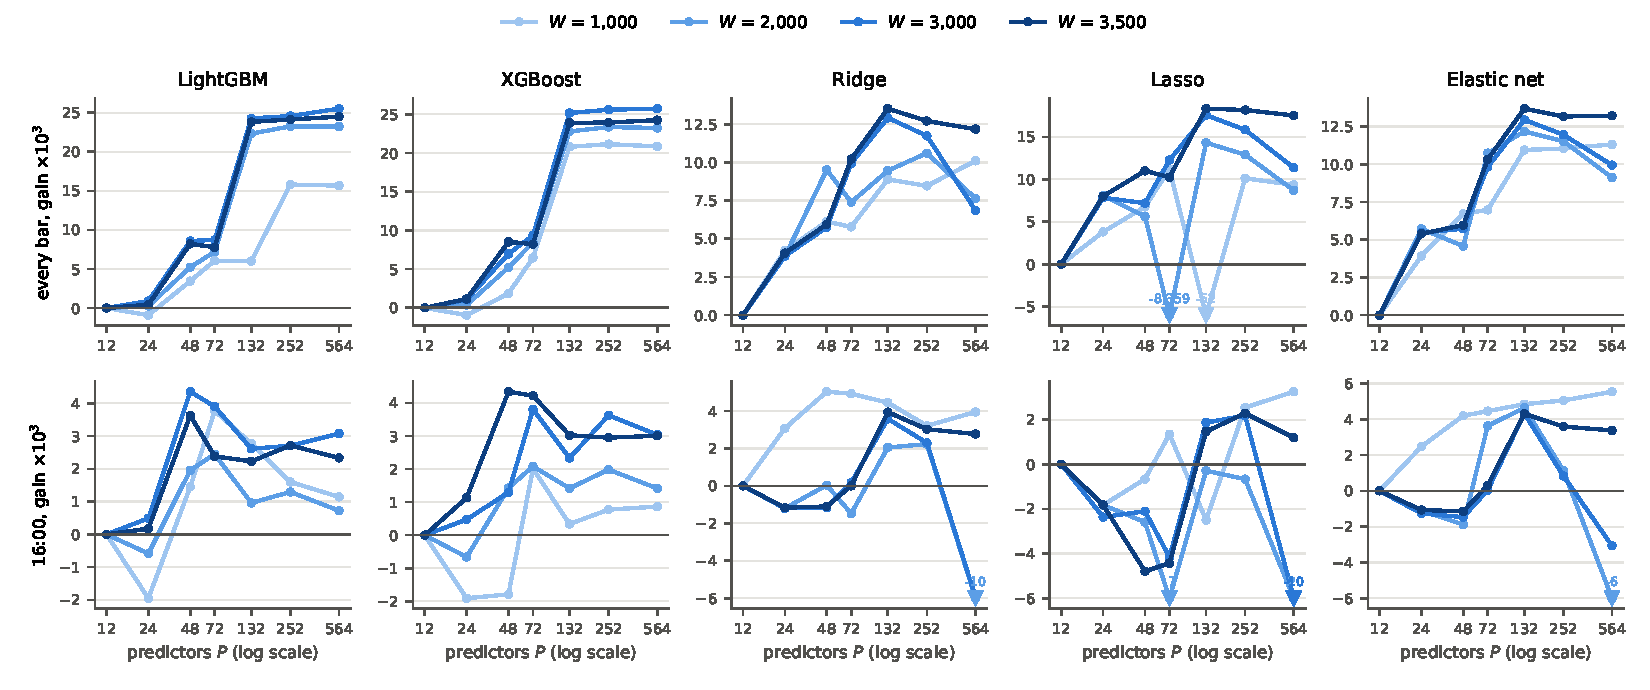
\includegraphics[width=\linewidth]{figures/rehaul_complexity_features.pdf}
  \caption{Feature scaling: the gain over the HAR benchmark set against the number of predictors $P = 12 + 12k$
    ($k = 0, 1, 3, 5, 10, 20, 46$ exogenous series), one line per rolling window ($W = \rhcxWOne$, \rhcxWTwo,
    \rhcxWMain{} and \rhcxWLong{} trading days, $T = 13W$ bars), one panel per model. Gain: QLIKE of the same
    window's $k = 0$ rung minus the rung's, $\times 10^3$, on the \rhcxNBars{} scored bars (top) and the 16:00 bar
    (bottom). Monthly refits at \rhcxNOrigins{} origins. FOMC-patched design.}
  \label{fig:rh_cx_features}
\end{figure}
\begin{figure}[tbp]
  \centering
  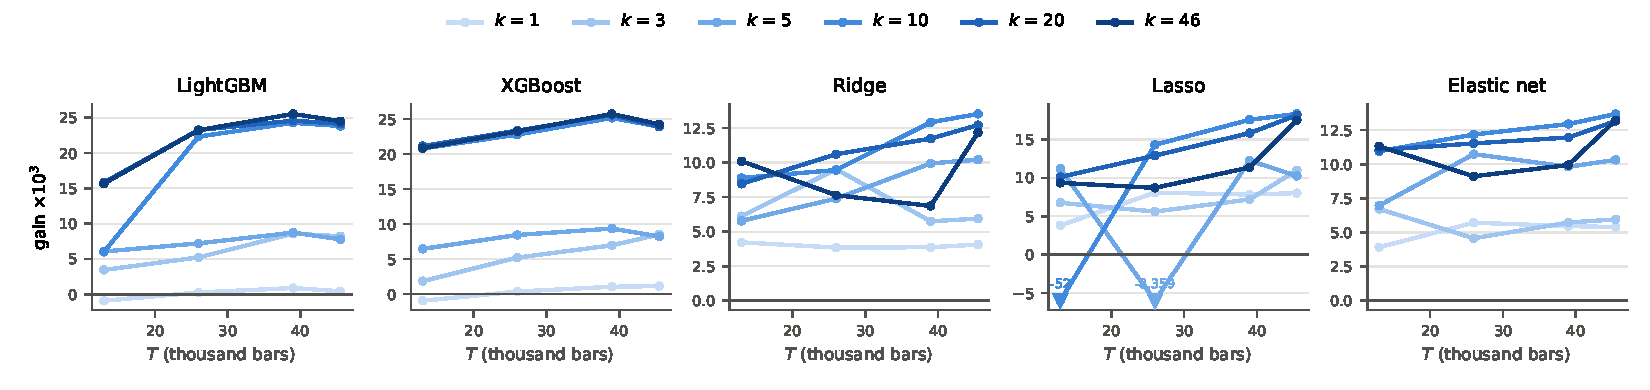
\includegraphics[width=\linewidth]{figures/rehaul_complexity_data.pdf}
  \caption{Data scaling: the gain over the same window's $k = 0$ rung against the window length $T$ at a fixed number
    of exogenous series $k$ (every bar). Same runs as Figure~\ref{fig:rh_cx_features}. FOMC-patched design.}
  \label{fig:rh_cx_data}
\end{figure}
 after the section.
% The pre-patch run's macros and floats are generated/rehaul_complexity_{numbers,floats}_prepatch.tex (same macro
% names: never input both).

\subsection{Window length, number of series and the exogenous gain (draft)}
\label{sec:rh_cx}
\editc{orange}{CX}{Draft for the author (2026-10-26): the scaling reading of the window $\times$ number-of-series grid,
on the FOMC-patched design, monthly refits.}
\begin{itemize}
\item \textbf{Question.} Does the gain from the exogenous series grow with the number of series a model sees and with
  the length of its training window, and does the number of series worth keeping grow with the window? If the
  exogenous signal were dense and weak, more data per parameter would let more of the weak series pay for themselves,
  so the best number of series would rise with the window.
\item \textbf{What is computed.}
  \begin{itemize}
  \item A grid of rolling windows $W = \rhcxWOne$, \rhcxWTwo, \rhcxWMain{} and \rhcxWLong{} trading days ($T = 13W$,
    from \rhcxTOne{} to \rhcxTLong{} bars) and of rungs $k = 0, 1, 3, 5, 10, 20, \rhcxNSeries$: each rung keeps the
    \rhcxPHar{} columns of the HAR benchmark set and all columns of the top $k$ exogenous series, so it has
    $P = 12 + 12k$ predictors (\rhcxPFull{} for the full set).
  \item The series are ranked separately at each window and for each model, by one fit before the evaluation span
    (origin 2 January 2013, explained on 2013: mean absolute SHAP value for the trees, $\sum |\beta|\,\mathrm{s.d.}$
    for the linear models). This is the first-training-window ranking of \citet{MaischZhangUlrichZimmer2026}.
  \item LightGBM and XGBoost on their frozen configurations at every window (minimum leaf sizes not rescaled with
    $T$); ridge, lasso and elastic net on each window's own frozen penalty (ridge \rhcxPenRidgeOne{} at $W =
    \rhcxWOne$, \rhcxPenRidgeMain{} at the other windows; lasso \rhcxPenLassoOne{} and \rhcxPenLassoMain; elastic net
    \rhcxPenEnetOne{} and \rhcxPenEnetMain).
  \item Each rung is refitted at the \rhcxNOrigins{} monthly origins of Section~\ref{sec:rh_fi} and held for the next
    21 sessions. At $W = \rhcxWMain$ the full rung equals the every-bar walk at every origin; at every window a rung
    without the FOMC proximity series equals its pre-patch twin bit for bit (\rhcxNGatesPass{} of \rhcxNGates{}
    window--model gates).
  \item Gain $G(W, k)$: the QLIKE of the same window's $k = 0$ rung minus the rung's, $\times 10^3$, on the
    \rhcxNBars{} scored bars of Table~\ref{tab:rh_oos} and on the 16:00 bar; Diebold--Mariano tests against $k = 0$
    (HLN, Newey--West lag \rhcxHacLag). Figures~\ref{fig:rh_cx_features} and~\ref{fig:rh_cx_data}.
  \end{itemize}
\item \textbf{Feature scaling (fixed window).}
  \begin{itemize}
  \item Trees: LightGBM at $W = \rhcxWMain$ gains \rhcxGainLgbmBarMainFive{} with 5 series, \rhcxGainLgbmBarMainTen{}
    with 10 and \rhcxGainLgbmBarMainFull{} with all \rhcxNSeries; XGBoost \rhcxGainXgbBarMainFive,
    \rhcxGainXgbBarMainTen{} and \rhcxGainXgbBarMainFull. The full set is the best rung in \rhcxNFullBestTreesBar{} of 8
    window--tree cells on every bar.
  \item Linear models: ridge at $W = \rhcxWMain$ gains \rhcxGainRidgeBarMainFive, \rhcxGainRidgeBarMainTen{} and
    \rhcxGainRidgeBarMainFull{} (5, 10 and all series); lasso \rhcxGainLassoBarMainFive, \rhcxGainLassoBarMainTen{}
    and \rhcxGainLassoBarMainFull; elastic net \rhcxGainEnetBarMainFive, \rhcxGainEnetBarMainTen{} and
    \rhcxGainEnetBarMainFull. The full set is the best rung in \rhcxNFullBestLinearBar{} of 12 window--linear cells.
  \end{itemize}
\item \textbf{Data scaling (fixed number of series).}
  \begin{itemize}
  \item LightGBM with 10 series: \rhcxGainLgbmBarOneTen{} at $W = \rhcxWOne$, \rhcxGainLgbmBarTwoTen{} at \rhcxWTwo,
    \rhcxGainLgbmBarMainTen{} at \rhcxWMain{} and \rhcxGainLgbmBarLongTen{} at \rhcxWLong; with all series
    \rhcxGainLgbmBarOneFull, \rhcxGainLgbmBarTwoFull, \rhcxGainLgbmBarMainFull{} and \rhcxGainLgbmBarLongFull.
  \item Ridge with 10 series: \rhcxGainRidgeBarOneTen, \rhcxGainRidgeBarTwoTen, \rhcxGainRidgeBarMainTen{} and
    \rhcxGainRidgeBarLongTen; with all series \rhcxGainRidgeBarOneFull, \rhcxGainRidgeBarTwoFull,
    \rhcxGainRidgeBarMainFull{} and \rhcxGainRidgeBarLongFull.
  \end{itemize}
\item \textbf{Does the best number of series rise with the window?} On every bar the rung with the lowest QLIKE at
  $W = \rhcxWOne$, \rhcxWTwo, \rhcxWMain{} and \rhcxWLong{} has $k^\ast = \rhcxKstarLgbmBarOne$, \rhcxKstarLgbmBarTwo,
  \rhcxKstarLgbmBarMain, \rhcxKstarLgbmBarLong{} series for LightGBM (it \rhcxKstarReadLgbmBar), \rhcxKstarXgbBarOne,
  \rhcxKstarXgbBarTwo, \rhcxKstarXgbBarMain, \rhcxKstarXgbBarLong{} for XGBoost (\rhcxKstarReadXgbBar),
  \rhcxKstarRidgeBarOne, \rhcxKstarRidgeBarTwo, \rhcxKstarRidgeBarMain, \rhcxKstarRidgeBarLong{} for ridge
  (\rhcxKstarReadRidgeBar), \rhcxKstarLassoBarOne, \rhcxKstarLassoBarTwo, \rhcxKstarLassoBarMain,
  \rhcxKstarLassoBarLong{} for the lasso (\rhcxKstarReadLassoBar) and \rhcxKstarEnetBarOne, \rhcxKstarEnetBarTwo,
  \rhcxKstarEnetBarMain, \rhcxKstarEnetBarLong{} for the elastic net (\rhcxKstarReadEnetBar).
  \begin{itemize}
  \item The dense-and-weak prediction, a best number of series that rises with the window, holds on every bar for
    \rhcxWhoKstarRisesBar{} and at the 16:00 bar for \rhcxWhoKstarRisesClose.
  \end{itemize}
\item \textbf{Caveats.}
  \begin{itemize}
  \item Two lasso cells are dominated by a few held forecasts near zero. At $W = \rhcxWTwo$ with 5 series
    (\rhcxGainLassoBarTwoFive) the five series are the same as before the patch, so the patched FOMC proximity columns
    alone cause it; the forecasts come from the origin of 3 March 2020, inside the period the FOMC fix rewrites. At
    $W = \rhcxWOne$ with 10 series (\rhcxGainLassoBarOneTen) they come from the origin of 30 June 2014. The lasso's best
    number of series at $W = \rhcxWOne$ (\rhcxKstarLassoBarOne) and its rise across windows reflect these blow-ups, not
    a preference.
  \item The window length is confounded with regime averaging: a longer window averages over more regimes. The
    linear penalties also change with the window (tenfold at $W = \rhcxWOne$), and the rankings are refitted at each
    window, so the series behind a given $k$ differ across windows.
  \item The trees' minimum leaf sizes are not rescaled with $T$, so a shorter window also means relatively larger
    leaves.
  \item Monthly refits held for 21 sessions, not the every-bar walks of Table~\ref{tab:rh_oos}. Holding a fit costs
    the full linear set most.
  \item Four windows with no intervals: descriptive.
  \end{itemize}
\end{itemize}

% ---------------------------------------------------------------------------------------------------------------------
% OPTIONAL related-work sentence (only if the paper mentions complexity at all; the author dropped that framing), for
% rehaul/02_related_work.tex, bullet "Shrinkage with many weak signals", after "... bears directly on the
% dense-versus-sparse question." (not applied):
%
%   \citet{KellyMalamudZhou2024} argue against parsimony in return prediction: a ridge regression on many more
%   random nonlinear features than observations (complexity $c = P/T > 1$) predicts better out of sample than simple
%   models, and its market-timing value rises with complexity even where the out-of-sample $R^2$ is poor.
% ---------------------------------------------------------------------------------------------------------------------
 where the subsection should go (e.g. after the dense-and-weak item of
% rehaul/08_feature_importance.tex), % AUTO-GENERATED by writeup/make_rehaul_complexity.py -- do not edit; re-run the script.
% Floats of the draft scaling subsection (writeup/drafts/2026-10-26_complexity.tex). PATCHED design: the FOMC fix adopted (FOMC_SCHEDULE_2020_FIX, FOMC_PROXIMITY_NO_WINSOR; RULE.txt ADDENDUM 3).
\begin{figure}[tbp]
  \centering
  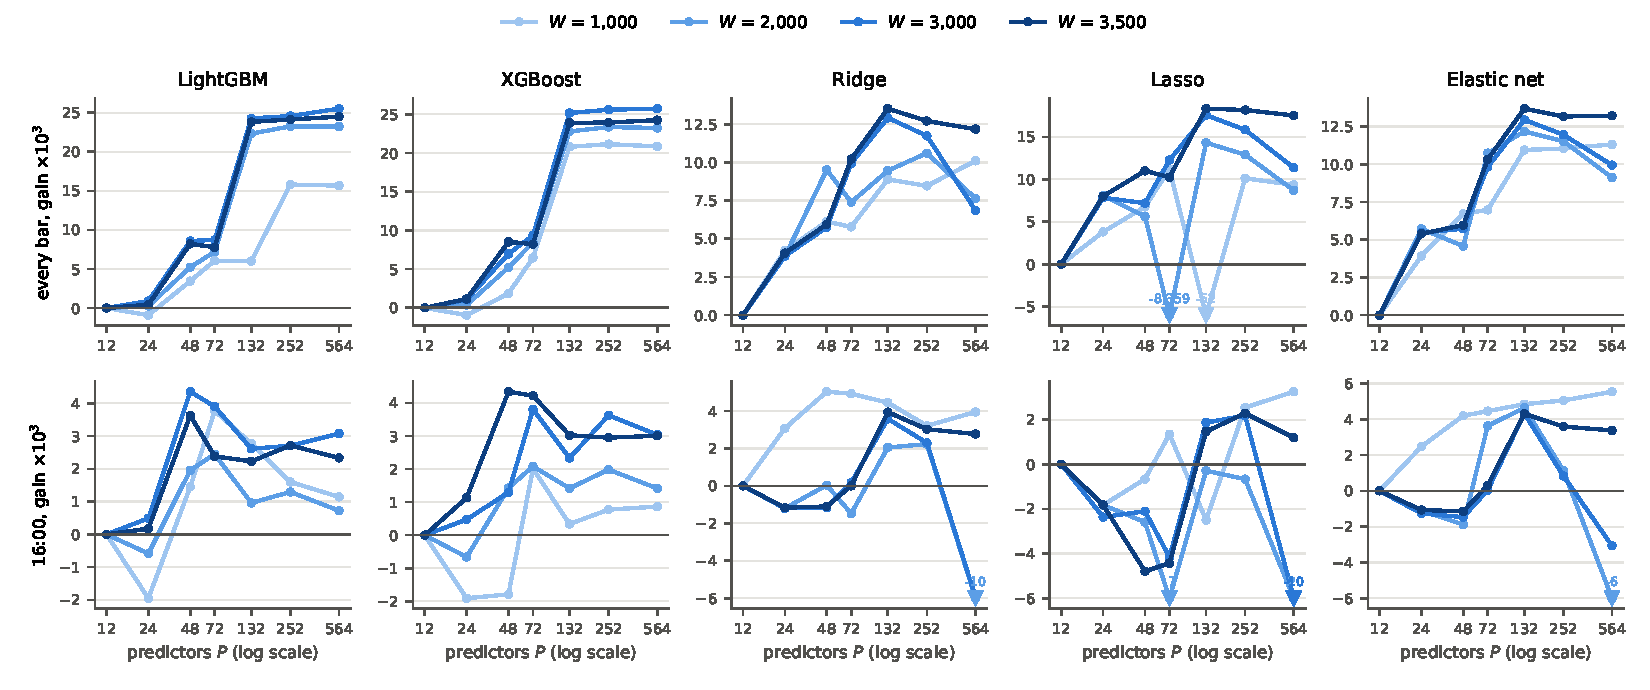
\includegraphics[width=\linewidth]{figures/rehaul_complexity_features.pdf}
  \caption{Feature scaling: the gain over the HAR benchmark set against the number of predictors $P = 12 + 12k$
    ($k = 0, 1, 3, 5, 10, 20, 46$ exogenous series), one line per rolling window ($W = \rhcxWOne$, \rhcxWTwo,
    \rhcxWMain{} and \rhcxWLong{} trading days, $T = 13W$ bars), one panel per model. Gain: QLIKE of the same
    window's $k = 0$ rung minus the rung's, $\times 10^3$, on the \rhcxNBars{} scored bars (top) and the 16:00 bar
    (bottom). Monthly refits at \rhcxNOrigins{} origins. FOMC-patched design.}
  \label{fig:rh_cx_features}
\end{figure}
\begin{figure}[tbp]
  \centering
  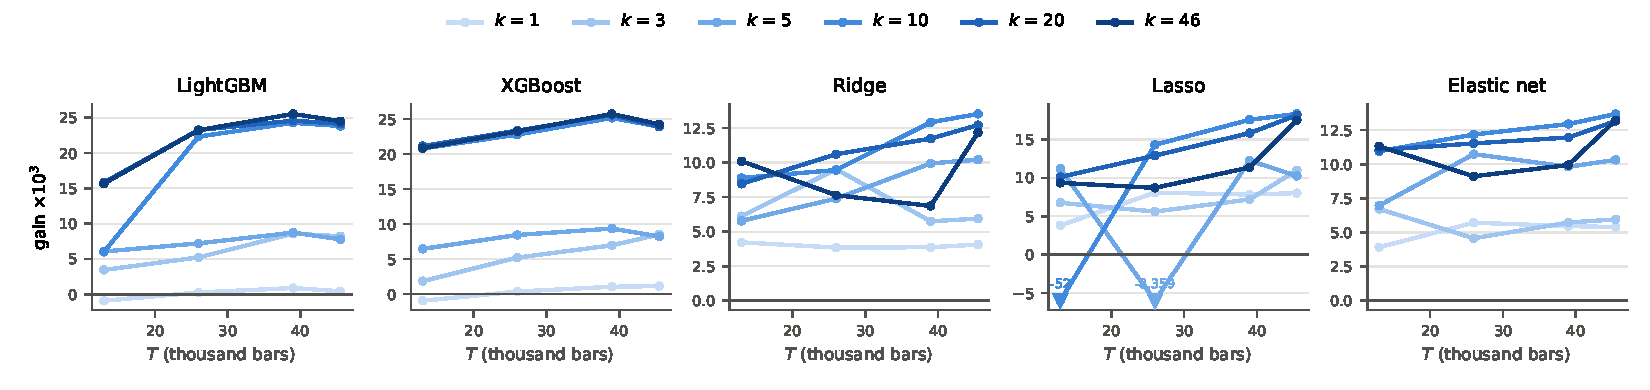
\includegraphics[width=\linewidth]{figures/rehaul_complexity_data.pdf}
  \caption{Data scaling: the gain over the same window's $k = 0$ rung against the window length $T$ at a fixed number
    of exogenous series $k$ (every bar). Same runs as Figure~\ref{fig:rh_cx_features}. FOMC-patched design.}
  \label{fig:rh_cx_data}
\end{figure}
 after the section.
% The pre-patch run's macros and floats are generated/rehaul_complexity_{numbers,floats}_prepatch.tex (same macro
% names: never input both).

\subsection{Window length, number of series and the exogenous gain (draft)}
\label{sec:rh_cx}
\editc{orange}{CX}{Draft for the author (2026-10-26): the scaling reading of the window $\times$ number-of-series grid,
on the FOMC-patched design, monthly refits.}
\begin{itemize}
\item \textbf{Question.} Does the gain from the exogenous series grow with the number of series a model sees and with
  the length of its training window, and does the number of series worth keeping grow with the window? If the
  exogenous signal were dense and weak, more data per parameter would let more of the weak series pay for themselves,
  so the best number of series would rise with the window.
\item \textbf{What is computed.}
  \begin{itemize}
  \item A grid of rolling windows $W = \rhcxWOne$, \rhcxWTwo, \rhcxWMain{} and \rhcxWLong{} trading days ($T = 13W$,
    from \rhcxTOne{} to \rhcxTLong{} bars) and of rungs $k = 0, 1, 3, 5, 10, 20, \rhcxNSeries$: each rung keeps the
    \rhcxPHar{} columns of the HAR benchmark set and all columns of the top $k$ exogenous series, so it has
    $P = 12 + 12k$ predictors (\rhcxPFull{} for the full set).
  \item The series are ranked separately at each window and for each model, by one fit before the evaluation span
    (origin 2 January 2013, explained on 2013: mean absolute SHAP value for the trees, $\sum |\beta|\,\mathrm{s.d.}$
    for the linear models). This is the first-training-window ranking of \citet{MaischZhangUlrichZimmer2026}.
  \item LightGBM and XGBoost on their frozen configurations at every window (minimum leaf sizes not rescaled with
    $T$); ridge, lasso and elastic net on each window's own frozen penalty (ridge \rhcxPenRidgeOne{} at $W =
    \rhcxWOne$, \rhcxPenRidgeMain{} at the other windows; lasso \rhcxPenLassoOne{} and \rhcxPenLassoMain; elastic net
    \rhcxPenEnetOne{} and \rhcxPenEnetMain).
  \item Each rung is refitted at the \rhcxNOrigins{} monthly origins of Section~\ref{sec:rh_fi} and held for the next
    21 sessions. At $W = \rhcxWMain$ the full rung equals the every-bar walk at every origin; at every window a rung
    without the FOMC proximity series equals its pre-patch twin bit for bit (\rhcxNGatesPass{} of \rhcxNGates{}
    window--model gates).
  \item Gain $G(W, k)$: the QLIKE of the same window's $k = 0$ rung minus the rung's, $\times 10^3$, on the
    \rhcxNBars{} scored bars of Table~\ref{tab:rh_oos} and on the 16:00 bar; Diebold--Mariano tests against $k = 0$
    (HLN, Newey--West lag \rhcxHacLag). Figures~\ref{fig:rh_cx_features} and~\ref{fig:rh_cx_data}.
  \end{itemize}
\item \textbf{Feature scaling (fixed window).}
  \begin{itemize}
  \item Trees: LightGBM at $W = \rhcxWMain$ gains \rhcxGainLgbmBarMainFive{} with 5 series, \rhcxGainLgbmBarMainTen{}
    with 10 and \rhcxGainLgbmBarMainFull{} with all \rhcxNSeries; XGBoost \rhcxGainXgbBarMainFive,
    \rhcxGainXgbBarMainTen{} and \rhcxGainXgbBarMainFull. The full set is the best rung in \rhcxNFullBestTreesBar{} of 8
    window--tree cells on every bar.
  \item Linear models: ridge at $W = \rhcxWMain$ gains \rhcxGainRidgeBarMainFive, \rhcxGainRidgeBarMainTen{} and
    \rhcxGainRidgeBarMainFull{} (5, 10 and all series); lasso \rhcxGainLassoBarMainFive, \rhcxGainLassoBarMainTen{}
    and \rhcxGainLassoBarMainFull; elastic net \rhcxGainEnetBarMainFive, \rhcxGainEnetBarMainTen{} and
    \rhcxGainEnetBarMainFull. The full set is the best rung in \rhcxNFullBestLinearBar{} of 12 window--linear cells.
  \end{itemize}
\item \textbf{Data scaling (fixed number of series).}
  \begin{itemize}
  \item LightGBM with 10 series: \rhcxGainLgbmBarOneTen{} at $W = \rhcxWOne$, \rhcxGainLgbmBarTwoTen{} at \rhcxWTwo,
    \rhcxGainLgbmBarMainTen{} at \rhcxWMain{} and \rhcxGainLgbmBarLongTen{} at \rhcxWLong; with all series
    \rhcxGainLgbmBarOneFull, \rhcxGainLgbmBarTwoFull, \rhcxGainLgbmBarMainFull{} and \rhcxGainLgbmBarLongFull.
  \item Ridge with 10 series: \rhcxGainRidgeBarOneTen, \rhcxGainRidgeBarTwoTen, \rhcxGainRidgeBarMainTen{} and
    \rhcxGainRidgeBarLongTen; with all series \rhcxGainRidgeBarOneFull, \rhcxGainRidgeBarTwoFull,
    \rhcxGainRidgeBarMainFull{} and \rhcxGainRidgeBarLongFull.
  \end{itemize}
\item \textbf{Does the best number of series rise with the window?} On every bar the rung with the lowest QLIKE at
  $W = \rhcxWOne$, \rhcxWTwo, \rhcxWMain{} and \rhcxWLong{} has $k^\ast = \rhcxKstarLgbmBarOne$, \rhcxKstarLgbmBarTwo,
  \rhcxKstarLgbmBarMain, \rhcxKstarLgbmBarLong{} series for LightGBM (it \rhcxKstarReadLgbmBar), \rhcxKstarXgbBarOne,
  \rhcxKstarXgbBarTwo, \rhcxKstarXgbBarMain, \rhcxKstarXgbBarLong{} for XGBoost (\rhcxKstarReadXgbBar),
  \rhcxKstarRidgeBarOne, \rhcxKstarRidgeBarTwo, \rhcxKstarRidgeBarMain, \rhcxKstarRidgeBarLong{} for ridge
  (\rhcxKstarReadRidgeBar), \rhcxKstarLassoBarOne, \rhcxKstarLassoBarTwo, \rhcxKstarLassoBarMain,
  \rhcxKstarLassoBarLong{} for the lasso (\rhcxKstarReadLassoBar) and \rhcxKstarEnetBarOne, \rhcxKstarEnetBarTwo,
  \rhcxKstarEnetBarMain, \rhcxKstarEnetBarLong{} for the elastic net (\rhcxKstarReadEnetBar).
  \begin{itemize}
  \item The dense-and-weak prediction, a best number of series that rises with the window, holds on every bar for
    \rhcxWhoKstarRisesBar{} and at the 16:00 bar for \rhcxWhoKstarRisesClose.
  \end{itemize}
\item \textbf{Caveats.}
  \begin{itemize}
  \item Two lasso cells are dominated by a few held forecasts near zero. At $W = \rhcxWTwo$ with 5 series
    (\rhcxGainLassoBarTwoFive) the five series are the same as before the patch, so the patched FOMC proximity columns
    alone cause it; the forecasts come from the origin of 3 March 2020, inside the period the FOMC fix rewrites. At
    $W = \rhcxWOne$ with 10 series (\rhcxGainLassoBarOneTen) they come from the origin of 30 June 2014. The lasso's best
    number of series at $W = \rhcxWOne$ (\rhcxKstarLassoBarOne) and its rise across windows reflect these blow-ups, not
    a preference.
  \item The window length is confounded with regime averaging: a longer window averages over more regimes. The
    linear penalties also change with the window (tenfold at $W = \rhcxWOne$), and the rankings are refitted at each
    window, so the series behind a given $k$ differ across windows.
  \item The trees' minimum leaf sizes are not rescaled with $T$, so a shorter window also means relatively larger
    leaves.
  \item Monthly refits held for 21 sessions, not the every-bar walks of Table~\ref{tab:rh_oos}. Holding a fit costs
    the full linear set most.
  \item Four windows with no intervals: descriptive.
  \end{itemize}
\end{itemize}

% ---------------------------------------------------------------------------------------------------------------------
% OPTIONAL related-work sentence (only if the paper mentions complexity at all; the author dropped that framing), for
% rehaul/02_related_work.tex, bullet "Shrinkage with many weak signals", after "... bears directly on the
% dense-versus-sparse question." (not applied):
%
%   \citet{KellyMalamudZhou2024} argue against parsimony in return prediction: a ridge regression on many more
%   random nonlinear features than observations (complexity $c = P/T > 1$) predicts better out of sample than simple
%   models, and its market-timing value rises with complexity even where the out-of-sample $R^2$ is poor.
% ---------------------------------------------------------------------------------------------------------------------
 where the subsection should go (e.g. after the dense-and-weak item of
% rehaul/08_feature_importance.tex), % AUTO-GENERATED by writeup/make_rehaul_complexity.py -- do not edit; re-run the script.
% Floats of the draft scaling subsection (writeup/drafts/2026-10-26_complexity.tex). PATCHED design: the FOMC fix adopted (FOMC_SCHEDULE_2020_FIX, FOMC_PROXIMITY_NO_WINSOR; RULE.txt ADDENDUM 3).
\begin{figure}[tbp]
  \centering
  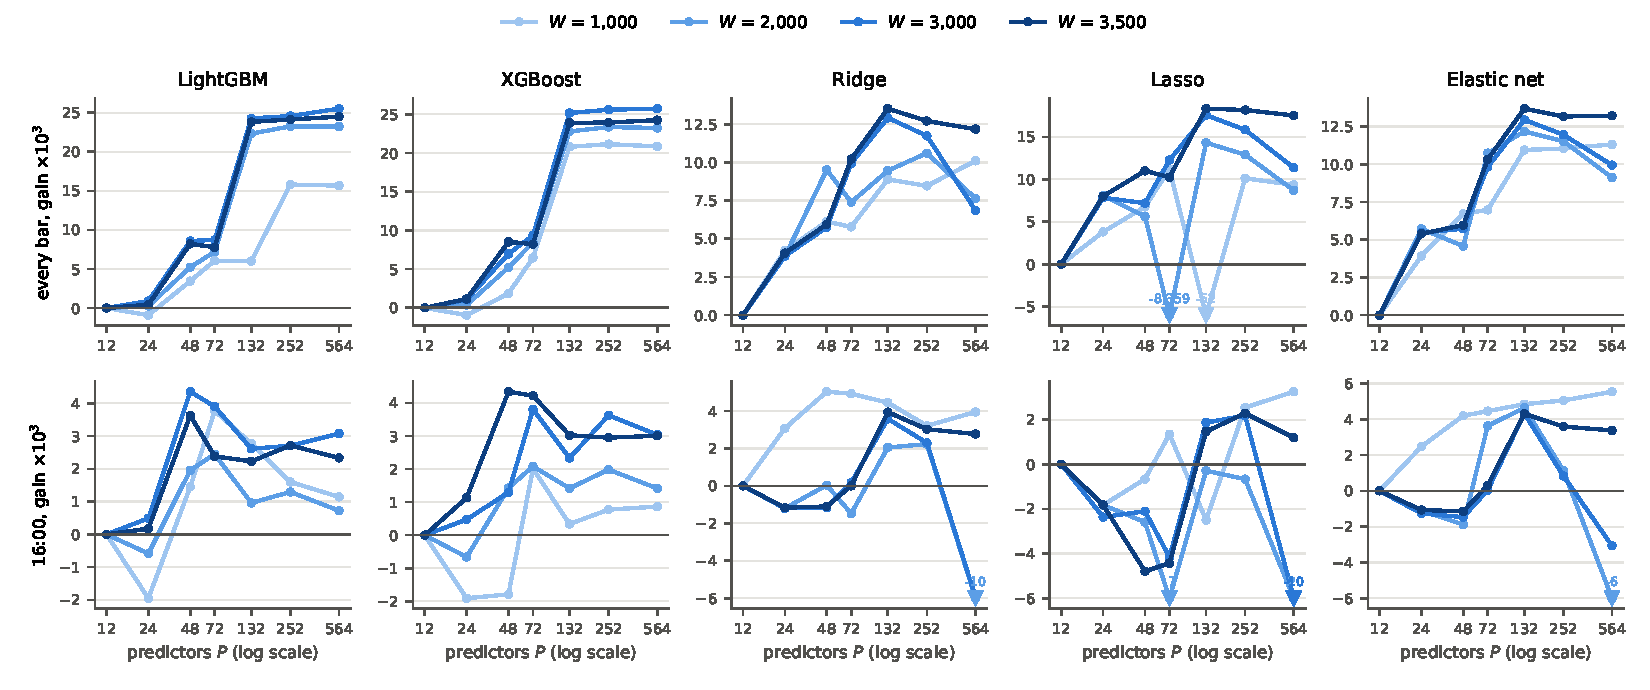
\includegraphics[width=\linewidth]{figures/rehaul_complexity_features.pdf}
  \caption{Feature scaling: the gain over the HAR benchmark set against the number of predictors $P = 12 + 12k$
    ($k = 0, 1, 3, 5, 10, 20, 46$ exogenous series), one line per rolling window ($W = \rhcxWOne$, \rhcxWTwo,
    \rhcxWMain{} and \rhcxWLong{} trading days, $T = 13W$ bars), one panel per model. Gain: QLIKE of the same
    window's $k = 0$ rung minus the rung's, $\times 10^3$, on the \rhcxNBars{} scored bars (top) and the 16:00 bar
    (bottom). Monthly refits at \rhcxNOrigins{} origins. FOMC-patched design.}
  \label{fig:rh_cx_features}
\end{figure}
\begin{figure}[tbp]
  \centering
  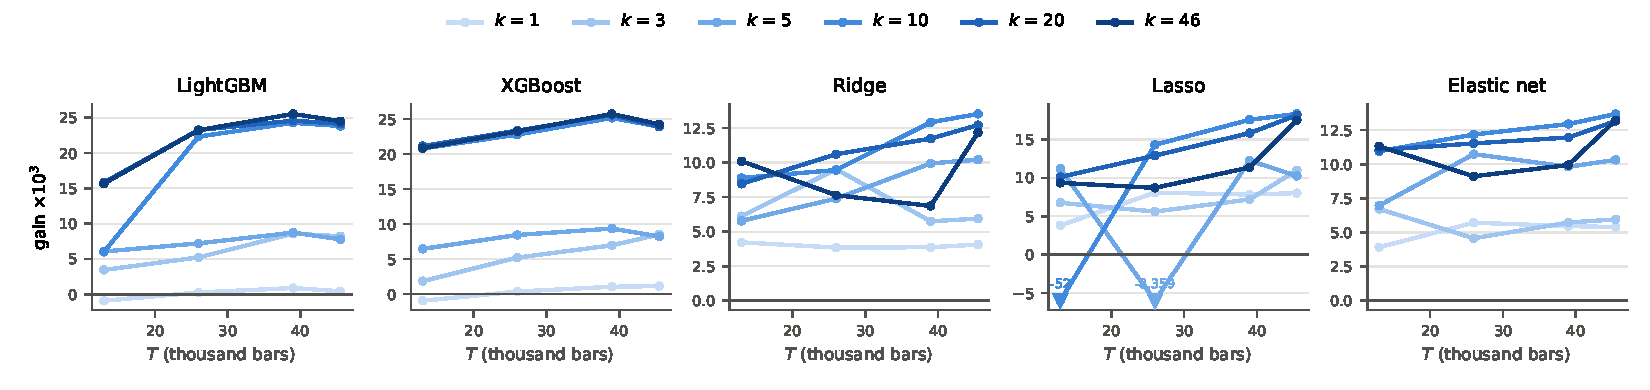
\includegraphics[width=\linewidth]{figures/rehaul_complexity_data.pdf}
  \caption{Data scaling: the gain over the same window's $k = 0$ rung against the window length $T$ at a fixed number
    of exogenous series $k$ (every bar). Same runs as Figure~\ref{fig:rh_cx_features}. FOMC-patched design.}
  \label{fig:rh_cx_data}
\end{figure}
 after the section.
% The pre-patch run's macros and floats are generated/rehaul_complexity_{numbers,floats}_prepatch.tex (same macro
% names: never input both).

\subsection{Window length, number of series and the exogenous gain (draft)}
\label{sec:rh_cx}
\editc{orange}{CX}{Draft for the author (2026-10-26): the scaling reading of the window $\times$ number-of-series grid,
on the FOMC-patched design, monthly refits.}
\begin{itemize}
\item \textbf{Question.} Does the gain from the exogenous series grow with the number of series a model sees and with
  the length of its training window, and does the number of series worth keeping grow with the window? If the
  exogenous signal were dense and weak, more data per parameter would let more of the weak series pay for themselves,
  so the best number of series would rise with the window.
\item \textbf{What is computed.}
  \begin{itemize}
  \item A grid of rolling windows $W = \rhcxWOne$, \rhcxWTwo, \rhcxWMain{} and \rhcxWLong{} trading days ($T = 13W$,
    from \rhcxTOne{} to \rhcxTLong{} bars) and of rungs $k = 0, 1, 3, 5, 10, 20, \rhcxNSeries$: each rung keeps the
    \rhcxPHar{} columns of the HAR benchmark set and all columns of the top $k$ exogenous series, so it has
    $P = 12 + 12k$ predictors (\rhcxPFull{} for the full set).
  \item The series are ranked separately at each window and for each model, by one fit before the evaluation span
    (origin 2 January 2013, explained on 2013: mean absolute SHAP value for the trees, $\sum |\beta|\,\mathrm{s.d.}$
    for the linear models). This is the first-training-window ranking of \citet{MaischZhangUlrichZimmer2026}.
  \item LightGBM and XGBoost on their frozen configurations at every window (minimum leaf sizes not rescaled with
    $T$); ridge, lasso and elastic net on each window's own frozen penalty (ridge \rhcxPenRidgeOne{} at $W =
    \rhcxWOne$, \rhcxPenRidgeMain{} at the other windows; lasso \rhcxPenLassoOne{} and \rhcxPenLassoMain; elastic net
    \rhcxPenEnetOne{} and \rhcxPenEnetMain).
  \item Each rung is refitted at the \rhcxNOrigins{} monthly origins of Section~\ref{sec:rh_fi} and held for the next
    21 sessions. At $W = \rhcxWMain$ the full rung equals the every-bar walk at every origin; at every window a rung
    without the FOMC proximity series equals its pre-patch twin bit for bit (\rhcxNGatesPass{} of \rhcxNGates{}
    window--model gates).
  \item Gain $G(W, k)$: the QLIKE of the same window's $k = 0$ rung minus the rung's, $\times 10^3$, on the
    \rhcxNBars{} scored bars of Table~\ref{tab:rh_oos} and on the 16:00 bar; Diebold--Mariano tests against $k = 0$
    (HLN, Newey--West lag \rhcxHacLag). Figures~\ref{fig:rh_cx_features} and~\ref{fig:rh_cx_data}.
  \end{itemize}
\item \textbf{Feature scaling (fixed window).}
  \begin{itemize}
  \item Trees: LightGBM at $W = \rhcxWMain$ gains \rhcxGainLgbmBarMainFive{} with 5 series, \rhcxGainLgbmBarMainTen{}
    with 10 and \rhcxGainLgbmBarMainFull{} with all \rhcxNSeries; XGBoost \rhcxGainXgbBarMainFive,
    \rhcxGainXgbBarMainTen{} and \rhcxGainXgbBarMainFull. The full set is the best rung in \rhcxNFullBestTreesBar{} of 8
    window--tree cells on every bar.
  \item Linear models: ridge at $W = \rhcxWMain$ gains \rhcxGainRidgeBarMainFive, \rhcxGainRidgeBarMainTen{} and
    \rhcxGainRidgeBarMainFull{} (5, 10 and all series); lasso \rhcxGainLassoBarMainFive, \rhcxGainLassoBarMainTen{}
    and \rhcxGainLassoBarMainFull; elastic net \rhcxGainEnetBarMainFive, \rhcxGainEnetBarMainTen{} and
    \rhcxGainEnetBarMainFull. The full set is the best rung in \rhcxNFullBestLinearBar{} of 12 window--linear cells.
  \end{itemize}
\item \textbf{Data scaling (fixed number of series).}
  \begin{itemize}
  \item LightGBM with 10 series: \rhcxGainLgbmBarOneTen{} at $W = \rhcxWOne$, \rhcxGainLgbmBarTwoTen{} at \rhcxWTwo,
    \rhcxGainLgbmBarMainTen{} at \rhcxWMain{} and \rhcxGainLgbmBarLongTen{} at \rhcxWLong; with all series
    \rhcxGainLgbmBarOneFull, \rhcxGainLgbmBarTwoFull, \rhcxGainLgbmBarMainFull{} and \rhcxGainLgbmBarLongFull.
  \item Ridge with 10 series: \rhcxGainRidgeBarOneTen, \rhcxGainRidgeBarTwoTen, \rhcxGainRidgeBarMainTen{} and
    \rhcxGainRidgeBarLongTen; with all series \rhcxGainRidgeBarOneFull, \rhcxGainRidgeBarTwoFull,
    \rhcxGainRidgeBarMainFull{} and \rhcxGainRidgeBarLongFull.
  \end{itemize}
\item \textbf{Does the best number of series rise with the window?} On every bar the rung with the lowest QLIKE at
  $W = \rhcxWOne$, \rhcxWTwo, \rhcxWMain{} and \rhcxWLong{} has $k^\ast = \rhcxKstarLgbmBarOne$, \rhcxKstarLgbmBarTwo,
  \rhcxKstarLgbmBarMain, \rhcxKstarLgbmBarLong{} series for LightGBM (it \rhcxKstarReadLgbmBar), \rhcxKstarXgbBarOne,
  \rhcxKstarXgbBarTwo, \rhcxKstarXgbBarMain, \rhcxKstarXgbBarLong{} for XGBoost (\rhcxKstarReadXgbBar),
  \rhcxKstarRidgeBarOne, \rhcxKstarRidgeBarTwo, \rhcxKstarRidgeBarMain, \rhcxKstarRidgeBarLong{} for ridge
  (\rhcxKstarReadRidgeBar), \rhcxKstarLassoBarOne, \rhcxKstarLassoBarTwo, \rhcxKstarLassoBarMain,
  \rhcxKstarLassoBarLong{} for the lasso (\rhcxKstarReadLassoBar) and \rhcxKstarEnetBarOne, \rhcxKstarEnetBarTwo,
  \rhcxKstarEnetBarMain, \rhcxKstarEnetBarLong{} for the elastic net (\rhcxKstarReadEnetBar).
  \begin{itemize}
  \item The dense-and-weak prediction, a best number of series that rises with the window, holds on every bar for
    \rhcxWhoKstarRisesBar{} and at the 16:00 bar for \rhcxWhoKstarRisesClose.
  \end{itemize}
\item \textbf{Caveats.}
  \begin{itemize}
  \item Two lasso cells are dominated by a few held forecasts near zero. At $W = \rhcxWTwo$ with 5 series
    (\rhcxGainLassoBarTwoFive) the five series are the same as before the patch, so the patched FOMC proximity columns
    alone cause it; the forecasts come from the origin of 3 March 2020, inside the period the FOMC fix rewrites. At
    $W = \rhcxWOne$ with 10 series (\rhcxGainLassoBarOneTen) they come from the origin of 30 June 2014. The lasso's best
    number of series at $W = \rhcxWOne$ (\rhcxKstarLassoBarOne) and its rise across windows reflect these blow-ups, not
    a preference.
  \item The window length is confounded with regime averaging: a longer window averages over more regimes. The
    linear penalties also change with the window (tenfold at $W = \rhcxWOne$), and the rankings are refitted at each
    window, so the series behind a given $k$ differ across windows.
  \item The trees' minimum leaf sizes are not rescaled with $T$, so a shorter window also means relatively larger
    leaves.
  \item Monthly refits held for 21 sessions, not the every-bar walks of Table~\ref{tab:rh_oos}. Holding a fit costs
    the full linear set most.
  \item Four windows with no intervals: descriptive.
  \end{itemize}
\end{itemize}

% ---------------------------------------------------------------------------------------------------------------------
% OPTIONAL related-work sentence (only if the paper mentions complexity at all; the author dropped that framing), for
% rehaul/02_related_work.tex, bullet "Shrinkage with many weak signals", after "... bears directly on the
% dense-versus-sparse question." (not applied):
%
%   \citet{KellyMalamudZhou2024} argue against parsimony in return prediction: a ridge regression on many more
%   random nonlinear features than observations (complexity $c = P/T > 1$) predicts better out of sample than simple
%   models, and its market-timing value rises with complexity even where the out-of-sample $R^2$ is poor.
% ---------------------------------------------------------------------------------------------------------------------
